
% \documentclass[blackref,approvalform,dvipsnames]{drexel-thesis}
\documentclass[draft,dvipsnames]{drexel-thesis}


\author{Jae Hoon Kim}
\title{Classifying Human Driving Behavior via Deep Neural Networks}
\DUTmonth{June}
\DUTyear{2017}
\degree{Master in Computer Science}
\advisor{Santiago~Onta\~{n}\'{o}n, Ph.D.}
\copyrighttext{\copyrighttextCCBYSA}

\usepackage[numbers,sort&compress]{natbib} % fancy citation extensions
\bibliographystyle{unsrtnat}


% \usepackage{fancyvrb} % nicer verbatim handling
% \DefineShortVerb{\|}  % \verb+TEXT+  ->  |TEXT|

\usepackage{xcolor}
\usepackage{colortbl,booktabs}
\usepackage{xspace}
\usepackage{multirow}
\usepackage{wrapfig} % text around figures
\usepackage{amssymb} % \mathbbstarcra
\usepackage[final]{listings} % algorithms formated in code
\usepackage{enumitem} % compact imte lists
\usepackage{subcaption} % for subfigure (figures side-by-side)
\usepackage{mathtools}
\usepackage{soul}
\usepackage[detect-all]{siunitx} % Aligning numbers by decimal points in table columns
\usepackage{bm}
\usepackage{multirow}

\usepackage{algorithm, soul}
\usepackage[noend]{algpseudocode}
\algnewcommand{\Break}{\textbf{break}}

\newcommand{\todo}[1]{{\color{red}{\tt #1}}}
% \newcommand{\toredo}[1]{{\leavevmode\color{Plum}#1}}
\newcommand{\toredo}[1]{#1}
\newcommand{\modified}[1]{{\leavevmode\color{blue}#1}}
% \newcommand{\modified}[1]{#1}
\newcommand{\highest}[1]{\textcolor{Maroon}{\textbf{#1}}}
\newcommand{\StarCraft}{\mbox{\textsc{StarCraft}}\xspace}
\newcommand{\BroodWar}{\textsc{StarCraft: Brood War}\xspace}
\newcommand{\WarCraft}{\mbox{\textsc{WarCraft}}\xspace}
\newcommand{\WarCraftII}{\mbox{\textsc{WarCraft II}}\xspace}
\newcommand{\WarCraftIII}{\mbox{\textsc{WarCraft III}}\xspace}
\newcommand{\Wargus}{\mbox{\textsc{Wargus}}\xspace}
\newcommand{\Spring}{\mbox{\textsc{Spring}}\xspace}
\newcommand{\BWTA}{\textsc{BWTA}\xspace}
\newcommand{\BWTAb}{\textsc{BWTA2}\xspace}
\newcommand{\BWAPI}{\textsc{BWAPI}\xspace}
\newcommand{\SparCraft}{\textsc{SparCraft}\xspace}
\newcommand{\Lanchester}{\mbox{\emph{TS-Lanchester}$^2$}\xspace}
\newcommand{\cop}{\textsc{COP}\xspace}
\newcommand{\Ghost}{\textsc{GHOST}\xspace}
\newcommand{\Nova}{\textsc{Nova}\xspace}




\begin{document}
\begin{preamble}

% \begin{dedications}
% We're in \iffinal{final}{draft} mode!
% \end{dedications}

% \begin{acknowledgments}
% bla bla bla
% \end{acknowledgments}

\tableofcontents
\listoftables
\listoffigures

% \iffinal{}{\newpage}

\begin{abstract}
The average person spends several hours a day behind the wheel of their vehicles, which are usually equipped with on-board computers capable of collecting real-time data concerning driving behavior. However, this data source has rarely been tapped for healthcare and behavioral research purposes. This MS thesis is done in the context of the {\em Diagnostic Driving} project, an NSF funded collaborative project between Drexel, Children Hospital of Philadelphia (CHOP) and the University of Central Florida that aims at studying the possibility of using driving behavior data to diagnose medical conditions.
%
Specifically, this paper introduces focuses on the classification of driving behavior data collected in a driving simulator using deep neural networks. The target classification task is to differentiate novice versus expert drivers. The paper presents a comparative study on using different variants of LSTM (Long-Short Term Memory networks) and Auto-encoder networks to deal with the fact that we have a small amount of labels (16 examples of people driving in the simulator, each labeled with an ``expert'' or ``inexpert'' label), but each simulator drive is high dimensional and too densely sampled (each drive consists of 100 variables sampled at 60Hz).
%
Our results show that using an intermediate number of neurons in the LSTM networks and using data filtering (only considering one out of each 10 samples) obtains better results, and that using Auto-encoders works worse than using manual feature selection.
\end{abstract}
\end{preamble}

\begin{thesis}



% ####################################################################################################################################
\chapter{Introduction}\label{chap:intro}
% ####################################################################################################################################
Most people spend several hours per day for driving vehicle when they go to work, school or shopping. Modern car systems collect real-time data of car status and driving behavior. Those recorded data is good source for healthcare and research but it has rarely been used. This paper is done in the context of the {\em Diagnostic Driving} project, an NSF funded collaborative project between Drexel, Children Hospital of Philadelphia and the University of Central Florida that aims at studying the possibility of using driving behavior data to diagnose medical conditions.

The paper focuses on the classification of driving simulation data from novice and expert drivers by three different neural network models. Two datasets are used on the paper. First dataset has 16 traces from four drivers: two are inexpert drivers and two are expert drivers. Each drivers drove four different tracks. Second dataset is from first dataset but only 23 features are selected from original dataset. Three models consist of Long-Short Term Memory (LSTM) network. First model uses second dataset to classify data. Second model uses single layer auto-encoder to reduce dimensions of first dataset then classifies it by LSTM. The last model uses multiple layer auto-encoder to reduce dimensions of first dataset then classifies it by LSTM.

Chapter \ref{chap:bg} introduces background knowledge for deep neural network including LSTM and Auto-encoder and compares three most popular deep learning libraries. Chapter \ref{chap:dataset} explains detail about dataset. Technical approach and three different neural networks used for experiments on the paper are described in Chapter \ref{chap:tech_approach}. On Chapter \ref{chap:result}, result from three different neural network models are compared and analyzed. The last chapter, Chapter \ref{chap:conclusion}, forms a conclusion. The chapter mentions limitation of auto-encoder and new way to train multiple layer auto-encoder.


% ====================================================================================================================================
% ====================================================================================================================================
\chapter{Background}\label{chap:bg}
% ====================================================================================================================================
% ====================================================================================================================================
This chapter presents the necessary background to understand the experiments presented later in the paper. This chapter is dived into three sections. First Section \ref{sec:DL} covers basic deep learning including recurrent neural network and auto-encoders. Second Section \ref{sec:DLL} compares deep learning libraries: DL4J, Theano, and Tensorflow. The last Section \ref{sec:MLDD} introduces current trends in machine learning for driving data.

\section{Deep Learning}\label{sec:DL}
This section covers basic concepts of deep learning. First Subsection \ref{subsec:basicDL} introduces deep learning, and next Section \ref{subsec:RNN} deals with recurrent neural networks and long short term memory neural networks (LSTMs). The last Subsection \ref{subsec:AE} covers auto-encoders.

\subsection{Basic Concepts}\label{subsec:basicDL}

\subsubsection{Artificial Neuron}\label{subsubsec:AN}
The concept of artificial neurons or perseptrons was introduced by Warren McCullock and Walter Pitts \cite{raschka2015python}. Initial artificial neurons are described as binary output logic gate from inputs. If sum of weighted inputs is greater than threshold, the output is 1. Otherwise, the output is 0.

\begin{figure}[t!]
    \centering
    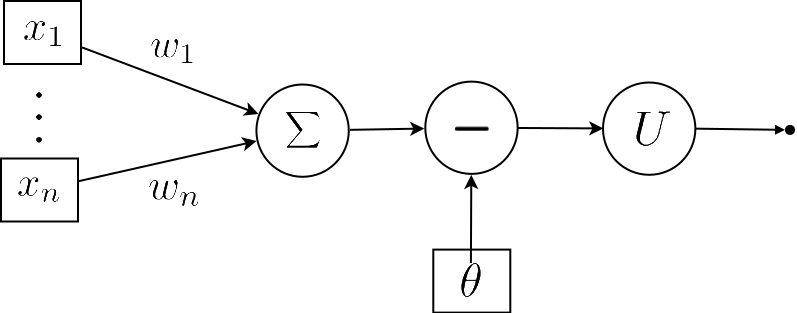
\includegraphics[width=0.65\textwidth]{pictures/figures/basic_AN.png}
    \caption{Basic Artificial Neuron}
    \label{fig:basic_AN}
\end{figure}

Figure \ref{fig:basic_AN} shows a basic artificial neuron. The input is $\vec{x} = \{x_1, ..., x_n\} \in \mathbb{R}^n$ and the weights for each input are $\vec{w} = \{w_1, ..., w_n\} \in \mathbb{R}^n$. Let $\theta$ be threshold and define step function as below:

$$U(z)=
	\begin{cases}
		\hfill 1 \hfill & \text{if $z > 0$} \\
		\hfill 0 \hfill & \text{otherwise} \\
	\end{cases}
$$

The function deciding output $o$ is called an activation function. In this case, the step function $U(z)$ is activation function.

Figure \ref{fig:basic_AN} also can be described by the following equation:
$$ o = U(\vec{x}\cdot\vec{w}-\theta)$$

\begin{figure}[t!]
    \centering
    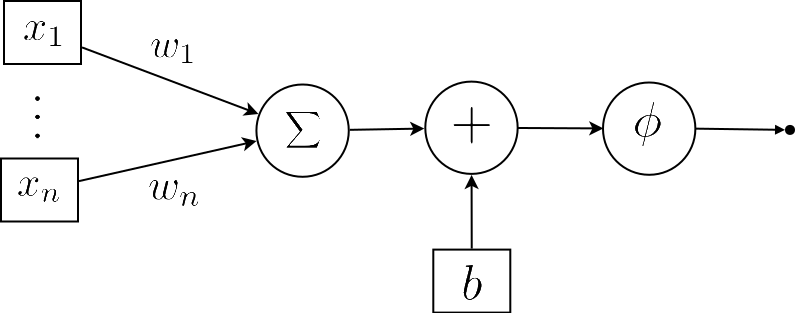
\includegraphics[width=0.65\textwidth]{pictures/figures/general_AN.png}
    \caption{General Artificial Neuron}
    \label{fig:general_AN}
\end{figure}

Figure \ref{fig:general_AN} shows an general artificial neuron. Threshold is replaced by bias and subtract node is replaced by add node. In general artificial neuron, activation function $\phi$ can be many different functions such as step, linear, or sigmoid function. An general artificial neuron also can be described by equation as follow:
$$o = \phi(\vec{x}\cdot\vec{w}+b)$$


\subsubsection{Neural Network}\label{subsubsec:NN}

\begin{figure}[t!]
    \centering
    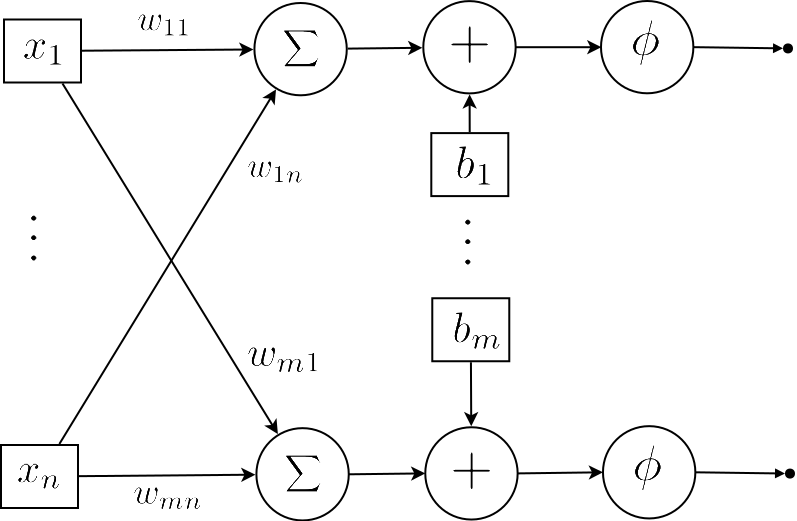
\includegraphics[width=0.65\textwidth]{pictures/figures/detail_NN.png}
    \caption{Single Layer in a Neural Network}
    \label{fig:detail_NN}
\end{figure}

Using single neuron has a limitation since it can solve only specific problems. For example, single neuron cannot solve xor problem. Instead of using single neuron, neural network has bundle of neurons. Figure \ref{fig:detail_NN} illustrates it with $n$ input and $m$ neurons. The input is $\vec{x} = \{x_1, ..., x_n\} \in \mathbb{R}^n$, weights for $i$th neuron are $\vec{w_i} = \{w_{i1}, ..., w_{in}\} \in \mathbb{R}^n$, and a bias term for the $i$th neuron is $b_i$. The output $\vec{o} = \{o_1, ..., o_m\} \in \mathbb{R}^m$ of the network is calculated as follows:
$$\vec{o} = \bm{\phi}(\{(\vec{x}\cdot\vec{w_1}+b_1),(\vec{x}\cdot\vec{w_2}+b_2),...,(\vec{x}\cdot\vec{w_m}+b_m)\})$$
Where activation function is applied on each element of its input.

To simplify the equation, let a transform matrix $\bold{w}: \mathbb{R}^n \rightarrow \mathbb{R}^m$ be
$\bold{w}=
\begin{bmatrix}
	\vec{w_1} & \vec{w_2} & \cdots & \vec{w_m}
\end{bmatrix}$
and bias vector $\vec{b} = \{b_1, ..., b_m\} \in \mathbb{R}^m$.

The equation is
$$\vec{o} = \bm{\phi}((\vec{x}^T\bold{w})^T+\vec{b})$$

The bias term can be skipped by extending input vector and weight transform matrix. Let $\vec{X} \in \mathbb{R}^{n+1}$ be $\{x_1, x_2, ..., x_n, 1\}$ which is added one more dimension from $\vec{x}$ with value 1 and $\vec{W_i} \in \mathbb{R}^{n+1}$ be $\{w_{i1}, ..., w_{in}, b_i\}$ which is added by bias term into weights and $\bold{W}: \mathbb{R}^{n+1} \rightarrow \mathbb{R}^m$ be
$\bold{W}=
\begin{bmatrix}
	\vec{W_1} & \vec{W_2} & \cdots & \vec{W_m}
\end{bmatrix}$

\begin{figure}[t!]
    \centering
    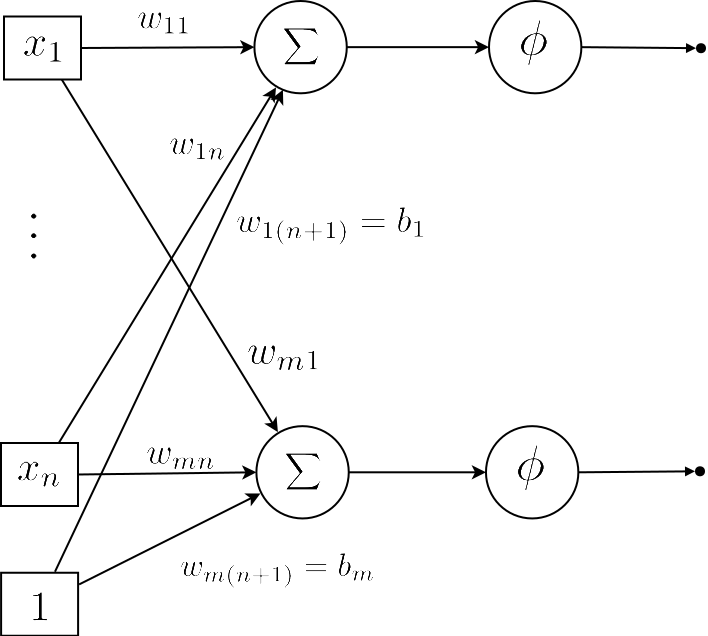
\includegraphics[width=0.75\textwidth]{pictures/figures/detail_NN_with_bias.png}
    \caption{Simplified Neural Network}
    \label{fig:withoutBiasNN}
\end{figure}

Figure \ref{fig:withoutBiasNN} shows same neural network as Figure \ref{fig:detail_NN} with $\vec{X}$ and $\bold{W}$. Notice that the figure does not have an added node anymore.

	From this point on the paper, vector in large case is with bias term and vector in small case is without bias term. For example, $\vec{X}$ is with bias and $\vec{x}$ is without bias. Also all vectors is row vector. Transform matrix is bold character and if it includes bias, transform matrix uses large case, otherwise small case. For example, $\bold{W}$ is transform matrix with bias and $\bold{w}$ is transform matrix without bias. By applying this, the equation for neural network is
$$\vec{o} = \bm{\phi}(\vec{X}\bold{W})$$

\begin{figure}[t!]
    \centering
    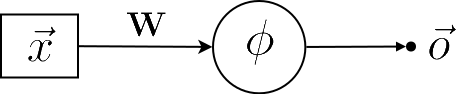
\includegraphics[width=0.4\textwidth]{pictures/figures/NN.png}
    \caption{Simplified Neural Network}
    \label{fig:NN}
\end{figure}

	For all figures under this point, $\Sigma$ node is skipped, square shape node represents input node, circle shape node represents compute node, edge with transform matrix represents weight matrix, edge without transform matrix represents identity matrix for weight matrix and arrow with small filled circle on end represents output vector. Figure \ref{fig:detail_NN}, Figure \ref{fig:withoutBiasNN}, and \ref{fig:NN} are equal.


\subsubsection{Multilayer Perceptron}\label{subsubsec:MLP}
Single layer perceptron neural network has only an input layer and an output layer such as Figure \ref{fig:NN} but multilayer perceptron (MLP) has several hidden layers between an input layer and an output layer. This part introduces to MLP by explaining neural network with one hidden layer. Let $\vec{x} \in \mathbb{R}^n$ be inputs, $\vec{h} \in \mathbb{R}^m$ be outputs from hidden layers, $\vec{c} \in \mathbb{R}^m$ be bias for hidden layers, $\vec{o} \in \mathbb{R}^l$ be outputs from an output layer, $\vec{b} \in \mathbb{R}^l$ be a bias for an output layer, $\bold{v}: \mathbb{R}^n \rightarrow \mathbb{R}^m$ be a transform matrix for hidden layers and $\bold{w}: \mathbb{R}^m \rightarrow \mathbb{R}^l$ be a transform matrix for an output layer. The activation function $\bold{f}()$ is for hidden layers and the activation function $\bold{g}()$ is for an output layer. Figure \ref{fig:MLP} shows one hidden layer MLP.

To compute output of MLP, forward-propagation is used. Forward-propagation is to pass inputs $\vec{x}$ to outputs through hidden layers \cite{murphy2012machine}. For example, the output from hidden layers on Figure \ref{fig:MLP} can be computed
$$\vec{h} = \bold{f}(\vec{x}\bold{v}+\vec{c}) = \bold{f}(\vec{X}\bold{V})$$
Then the output layer uses outputs from hidden layer as inputs. The outputs of the neural network can be computed
$$\vec{o} = \bold{g}(\vec{h}\bold{w}+\vec{b}) = \bold{g}(\vec{H}\bold{W})$$
Therefore, a final equation for two layer neural network is
$$\vec{o} = \bold{g}(\bold{h}(\vec{x}\bold{v}+\vec{c})\bold{w}+\vec{b}) = \bold{g}(\bold{h}(\vec{X}\bold{V})\bold{W})$$

\begin{figure}[t!]
    \centering
    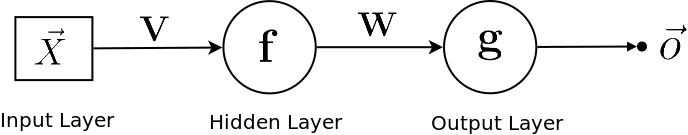
\includegraphics[width=0.5\textwidth]{pictures/figures/MLP.png}
    \caption{One Hidden Layer MLP}
    \label{fig:MLP}
\end{figure}


\subsubsection{Back-propagation}\label{subsubsec:BP}
Training neural network means finding weights and biases. Similar as forward-propagation, back-propagation is used when MLP is trained. As forward-propagation passes inputs $\vec{x}$ to outputs, back-propagation passes an error from the output layer to hidden layers \cite{murphy2012machine}. An error function $E()$ (some times called a loss function) usually uses a sum square error as follow:
$$E(\vec{y}, \vec{o}) = \frac{1}{2}\sum_{i}(y_i-o_i)^2$$
where $\vec{y}$ is an expected output from MLP.

Training neural network means finding weights and biases that make $\vec{o}$ close to $\vec{y}$. It means that training neural network needs a function of weights and biases. The train function $J()$ to train a neural network can be defined from error function $E()$. The error function $E()$ is a function of expected output and output from neural network with fixed weights and biases. Let weights and biases be changeable and the input be fixed on the error function, then the output is depends on weights and biases and the trained function $J()$ for one hidden MLP (Figure \ref{fig:MLP}) can be define below:
$$J(\bold{V}, \bold{W}) = \frac{1}{2}\sum_{i}(y_i-o_i)^2 = \frac{1}{2}\sum_{i}(y_i-g(\vec{H}\bold{W_i})^2 =\frac{1}{2}\sum_{i}(y_i-g(\bold{h}(\vec{X}\bold{V})\bold{W_i}))^2$$
where $\bold{W_i}$ is $i$th column of $\bold{W}$

The training function $J()$ for one hidden layer MLP is a function of $\bold{V}$ and $\bold{W}$ with fixed input. Again capital letter of transform matrix contains bias. So $\bold{V}$ is weights and biases for hidden layer and $\bold{W}$ is weights and biases for output layer.

To train the neural network, weights and biases are regulated. To update weights and biases, let $\vec{h'}=\vec{X}\bold{V}$ be inputs for a hidden layer activation function $\bold{f}$ and $\vec{o'}=\vec{H}\bold{W}$ be inputs for an output layer activation function $\bold{g}$. So $\vec{h}=\bold{f}(\vec{h'})=\bold{f}(\vec{X}\bold{V})$ and $\vec{o}=\bold{g}(\vec{o'})=\bold{g}(\vec{H}\bold{W})$. Let $V_{ij}$ be $i$th neuron weights in hidden layers for inputs  $X_j$ and $W_{ij}$ be $i$th neuron weight in an output layer for inputs $H_j$.

\begin{figure}[t!]
    \centering
    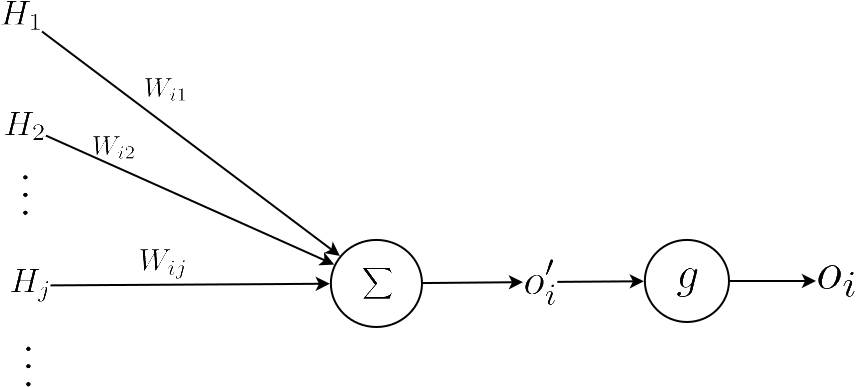
\includegraphics[width=0.7\textwidth]{pictures/figures/BP1.png}
    \caption{Back-propagation for $W_{ij}$}
    \label{fig:BP1}
\end{figure}

Let's first update $W_{ij}$ and Figure \ref{fig:BP1} shows the detail of an output layer related with ${W_{ij}}$. The updated weight ${{W_{ij}}^{next}}$ can be calculated as follow:
$${{W_{ij}}^{next}}=W_{ij} - \eta\frac{\partial J}{\partial W_{ij}}$$ where $\eta$ is a learning rate. The equation tells to remove error, updated weight should be move opposite direction of gradient of error function. The method is called 'gradient descent'.

Let's compute $\frac{\partial J}{\partial W_{ij}}$
$$
\frac{\partial J}{\partial W_{ij}}
= \frac{\partial J}{\partial o_i}\frac{\partial o_i}{\partial W_{ij}}
= \frac{\partial J}{\partial o_i}\frac{\partial o_i}{\partial o'_i}\frac{\partial o'_i}{\partial W_{ij}}
$$
So the equation has three parts.

First part is
$$
\frac{\partial o'_i}{\partial W_{ij}}
= \frac{\partial}{\partial W_{ij}}\sum_k(H_kW_{ik})
= \frac{\partial}{\partial W_{ij}}(H_jW_{ij})
= H_j
$$

Assume the activation function for an output layer is a sigmoid function $sigm()$ then the second part is
$$
\frac{\partial o_i}{\partial o'_i}
= \frac{\partial}{\partial o'_i}sigm(o'_i)
= sigm(o'_i)\{1-sigm(o'_i)\}
= o_i(1-o_i)
$$

Assume train function is sum square then the last part is
$$
\frac{\partial J}{\partial o_i}
= \frac{\partial}{\partial o_i}\frac{1}{2}\sum_k(y_k-o_k)^2
= \frac{\partial}{\partial o_i}\frac{1}{2}(y_i-o_i)^2
= -(y_i-o_i)
$$

Therefore,
$$
{{W_{ij}}^{next}}
= W_{ij} - \eta\frac{\partial J}{\partial W_{ij}}
= W_{ij} - \eta\frac{\partial J}{\partial o_i}\frac{\partial o_i}{\partial o'_i}\frac{\partial o'_i}{\partial W_{ij}}
= W_{ij} + \eta(y_i-o_i)o_i(1-o_i)H_j
$$

Before moving to update weights for hidden layer, define $\delta_i$ as follow:
$$
\delta_i
= \frac{\partial J}{\partial o'_i}
= \frac{\partial J}{\partial o_i}\frac{\partial o_i}{\partial o'_i}
$$

The $\delta_i$ is useful because it is shared when back-propagation updates all weights related with $i$th neuron. Also the $\delta_i$ is used when back-propagation updates weights on hidden layers.

\begin{figure}[t!]
    \centering
    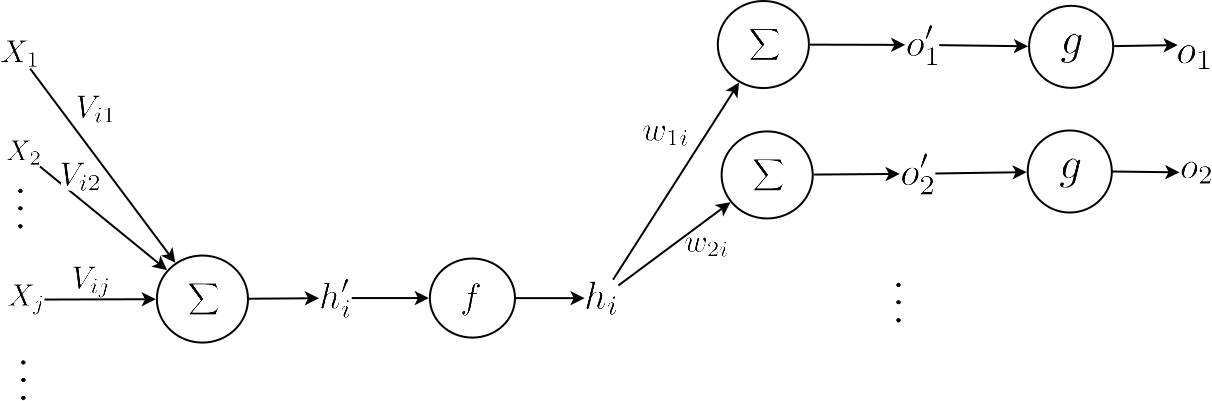
\includegraphics[width=\textwidth]{pictures/figures/BP2.png}
    \caption{Back-propagation for $V_{ij}$}
    \label{fig:BP2}
\end{figure}

The next step is to update weights in hidden layers. Let's update $V_{ij}$ and Figure \ref{fig:BP2} shows the detail of neural network related with $V_{ij}$. The updated weight ${{V_{ij}}^{next}}$ can be calculated as follow:
$${{V_{ij}}^{next}}=V_{ij} - \eta\frac{\partial J}{\partial V_{ij}}$$ where $\eta$ is a learning rate. The equation is similar as ${{W_{ij}}^{next}}$

Let's compute $\frac{\partial J}{\partial V_{ij}}$
$$
\frac{\partial J}{\partial V_{ij}}
= \frac{\partial J}{\partial h'_i}\frac{\partial h'_i}{\partial V_{ij}}
= \frac{\partial J}{\partial h_i}\frac{\partial h_i}{\partial h'_i}\frac{\partial h'_i}{\partial V_{ij}}
$$
So the equation also has three parts.

First part is
$$
\frac{\partial h'_i}{\partial V_{ij}}
= \frac{\partial}{\partial V_{ij}}\sum_k(X_kV_{ik})
= \frac{\partial}{\partial V_{ij}}(X_jV_{ij})
= X_j
$$

Assume the activation function for hidden layers is also a sigmoid function $sigm()$ then the second part is
$$
\frac{\partial h_i}{\partial h'_i}
= \frac{\partial}{\partial h'_i}sigm(h_i)
= sigm(h'_i)\{1-sigm(h'_i)\}
= h_i(1-h_i)
$$

Then the last part is
$$
\frac{\partial J}{\partial h_i}
= \sum_k(\frac{\partial J}{\partial o'_k}\frac{\partial o'_k}{\partial h_i})
= \sum_k(\delta_kw_{ki})
$$

Therefore,
$$
{{V_{ij}}^{next}}
= V_{ij} - \eta\frac{\partial J}{\partial V_{ij}}
= W_{ij} - \eta\frac{\partial J}{\partial h_i}\frac{\partial h_i}{\partial h'_i}\frac{\partial h'_i}{\partial V_{ij}}
= W_{ij} - \eta\sum_k(\delta_kw_{ki})h_i(1-h_i)X_j
$$

Notice that as forward-propagation sends output of a layer as input of the next layer, back-propagation sends the error of a the layer to the previous layer. For example, if the $\delta_i=\frac{\partial J}{\partial o'_i}$ is an error on the output layer, then it is sent to hidden layers.




\subsection{Recurrent Neural Network}\label{subsec:RNN}

\subsubsection{Basic concepts of recurrent neural networks:}\label{basicRNN}
	A recurrent neural network (RNN) is a neural network that is specialized for processing a sequence of input values \cite{Goodfellow-et-al-2016}. Figure \ref{fig:RNN} illustrates an abstract structure of RNN. RNN has two inputs. One input is from data such as a normal neural network input but the other input is from the previous output. The property gives benefit for sequential input data. This is because past outputs affect the current output. With sequential data, the previous data can affect the current data and RNN considers the previous outputs for the current output. It means that even the inputs from the data are equal, if the previous outputs are different, the current output are also different.

\begin{figure}[t!]
    \centering
    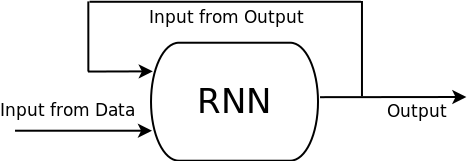
\includegraphics[width=0.5\textwidth]{pictures/figures/RNN.png}
    \caption{RNN}
    \label{fig:RNN}
\end{figure}

	For example, human language sentences have series of words, and meanings of words are different depending on context. RNN can be used for that. Another example is driving data which is used later on the paper.  Driving data are multi-dimension data with time domain. RNN can be used for the data because it is sequential data with the time domain.

	To describe RNN in a mathematical equation, let $\vec{x^t} = \{ x_1^t, ..., x_n^t\} \in \mathbb{R}^n$ be a vector that represents the input data at time $t$, $\vec{h^t} = \{ h_1^t, ..., h_m^t\} \in \mathbb{R}^m$ be result from hidden layer on time $t$, and $\vec{o^t} = \{ o_1^t, ..., o_l^t\} \in \mathbb{R}^l$ be output on time $t$. For transform matrix, let $\bold{u}: \mathbb{R}^n \rightarrow \mathbb{R}^m$ be a transform matrix for input data, $\bold{v}: \mathbb{R}^m \rightarrow \mathbb{R}^l$ be a transform matrix for data from hidden layer, and $\bold{w}: \mathbb{R}^l \rightarrow \mathbb{R}^m$ be a transform matrix for previous output. Figure \ref{fig:unfold_RNN} illustrates unfolded RNN with defined symbols. The result from hidden layer can be calculated by
	$$\vec{h^t} = \bold{f}(\vec{X^t}\bold{U} + \vec{O^{t-1}}\bold{W})$$ where $\bold{f}$ is an activation function for the hidden layer. Then the output can be calculated by
	$$\vec{o^t} = \bold{g}(\vec{H^t}\bold{V})$$ where $\bold{g}$ is an activation function for the output layer. Therefore, the RNN with bias is
	$$\vec{o^t} = \bold{g}(\bold{f}(\vec{x^t}\bold{u}+\vec{b_x} + \vec{o^{t-1}}\bold{w}+\vec{b_o})\bold{v}+\vec{b_h})$$ where $\vec{b_x} = \{b_{x1}, ..., b_{xm}\} \in \mathbb{R}^m$ is the bias for the input data, $\vec{b_o} = \{b_{o1}, ..., b_{om}\} \in \mathbb{R}^m$ is the bias for the previous output data, and $\vec{b_h} = \{b_{h1}, ..., b_{hl}\} \in \mathbb{R}^l$ is the bias for the data from the hidden layers.

\begin{figure}[t!]
    \centering
    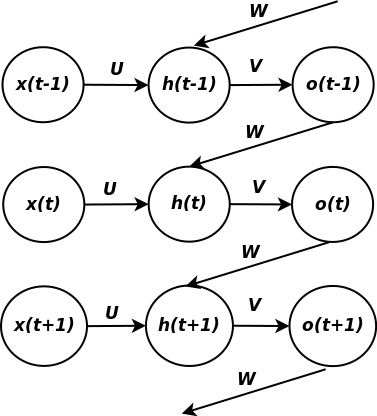
\includegraphics[width=0.65\textwidth]{pictures/figures/unfold_RNN.png}
    \caption{Unfold RNN}
    \label{fig:unfold_RNN}
\end{figure}

	RNN is not always like Figure \ref{fig:unfold_RNN}. Input from the previous output can be replaced by the result of the previous hidden layer. The main idea of RNN is that when neural network decides a current output, it considers a previous state.


\subsubsection{Long Short Term Memory (LSTM) networks:}\label{LSTM}
	Basic RNN has some problems of long term dependency. When RNN passes the previous output for the current output, some information in the input might or might be needed for future. RNN does not have an ability to filter unnecessary information or to store necessary information. Long Short Term Memory (LSTM) neural network can handle these problems.

	LSTM is a type of RNN introduced by Hochreiter and Schmidhuber \cite{hochreiter1997long}. LSTM solves long term dependency problems in RNN by memory cells. LSTM manages memory cells as a storage of knowledge. LSTM filters unnecessary information from memory cells and records necessary information on memory cells.

	The structure of LSTM consists of four gates: forget gate, input gate, input modulation gate, and output gate. Each gates have different purposes and Christopher Olah's blog \footnote{\url{http://colah.github.io/posts/2015-08-Understanding-LSTMs}} develops an intuition for the concept of LSTM and explains the purpose of each gates. The paper \cite{zaremba2014recurrent}  describes LSTM in a mathematical term. Let us first provide an intuitive description of how LSTM works by following Christopher Olah's blog, before providing a more in-depth formalization.

%	Bengio mentioned on his paper \cite{bengio2009learning} that each layer in deep neural network should have {\color{red} a} purpose. LSTM can be divided into four layers: forget gate, input gate, input modulation gate, and output gate. Each layer have different purposes {\color{red} [santi: this paragraph does not flow very well], even if Bengio mentioned it, why is it important? you need to explain WHY is it that each layer should have a purpose. Otherwise, we just have to believe in Bengio :)}.


\begin{enumerate}
\item An intuitive explanation of LSTMs:

	The easiest way to understand LSTM is to understand memory cell and the purpose of four different gates. Memory cells are what make LSTM different from RNN. Memory cells store important information and filter unimportant information for future. Three of four gates are involved in the memory cells to store and filter information.

	The first gate affecting memory cells is a forget gate. The forget gate decides unnecessary data from input data and previous output then applies it to memory cells. Other two gates are an input gate and an input modulation gate and these also influence memory cells. The two gates decide what information to remember to apply to memory cells. The last gate is an output gate and it does not directly affect memory cells. The output gate also has two inputs from the input data and the previous output, and outputs from the output gate is multiplied by memory cells to make a final output. Figure \ref{fig:LSTM} illustrates LSTM neural network with four gates and next part describes more detail of LSTM and the figure in a mathematical terms.

\begin{figure}[t!]
    \centering
    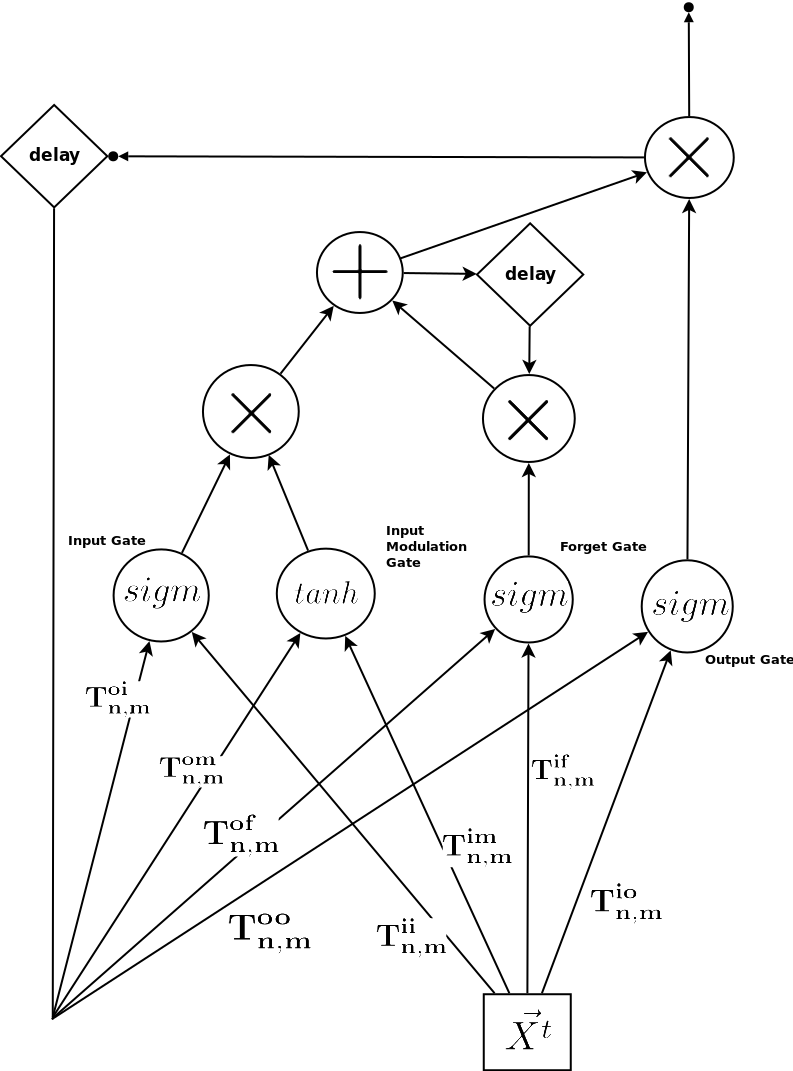
\includegraphics[width=0.75\textwidth]{pictures/figures/LSTM.png}
    \caption{LSTM}
    \label{fig:LSTM}
\end{figure}

		% It consists of sigmoid {\color{red} [santi: instead of saying ``It consists of sigmoid'', you should say something like ``The units in this layer use a sigmoid activation function'' (same comment for all the other layers below)]} layer with previous output and current input data {\color{red} [santi: a reader not familiar with LSTMs will not know what is ``previous output'' or ``current input'', so you need a figure that explains it]}. The result of the forget gate is multiplied by previous cell state to build current cell state.

		% The second layer is input gate and also consists of sigmod layer with previous output and current input data. The result of the input gate is multiplied by the result of input modulation gate then it affects to cell state {\color{red} [santi: all of these terms should appear in a figure, otherwise, a reader not familiar with it will not understand what you are saying. But also, even if you have a figure, you need to explain what each term is, e.g., explain what is ``input modulation'', what is ``cell state'', etc.]}. The meaning of input gate is to decide{\color{red} \st{s}} what data to remember.

		% The third layer is input modulation gate. It consists of tanh with previous output and current input. It is multiplied by the result of second layer and affects to current cell state.

		% The last layer is output gate. The layer decides what data should be passed to current output from previous output and current input. the output gate also consists of sigmoid with two inputs: last output and current input. The result of the layer is multiplied by current cell state passed tanh.

\item Modeling LSTMs in mathematical terms:

	To describe LSTM in a mathematical terms, let $\vec{x^t} = \{ x_1^t, ..., x_n^t\} \in \mathbb{R}^n$ be a vector that represents the input data at time $t$, $\vec{i^t} = \{i_1^t, ..., i_m^t\} \in \mathbb{R}^m$ be a result from an input gate on time $t$, $\vec{m^t} = \{m_1^t, ..., m_m^t\} \in \mathbb{R}^m$ be a result from an input modulation gate on time $t$, $\vec{f^t} = \{f_1^t, ..., f_m^t\} \in \mathbb{R}^m$ be a result from a forget gate on time $t$, $\vec{o^t} = \{o_1^t, ..., o_m^t\} \in \mathbb{R}^m$ be a result from an output gate on time $t$, $\vec{c^t} = \{c_1^t, ..., c_m^t\} \in \mathbb{R}^m$ be memory cells on time $t$, and $\vec{h^t} = \{h_1^t, ..., h_m^t\} \in \mathbb{R}^m$ be a final result on time $t$.
Each gate has transform matrices for inputs. Let $\bold{t_{n,m}}: \mathbb{R}^n \rightarrow \mathbb{R}^m$ be a transform matrix from $n$ dimension to $m$ dimension. Let $\bold{t_{n,m}^{ii}}$ be a transform matrix for the input from data in the input gate, $\bold{t_{m,m}^{oi}}$ be a transform matrix for the input from the previous output in the input gate, $\bold{t_{n,m}^{im}}$ be a transform matrix for the input from the data in the input modulation gate, $\bold{t_{m,m}^{om}}$ be a transform matrix for the input from the previous output in the input modulation gate, $\bold{t_{n,m}^{if}}$ be a transform matrix for the input from the data in the forget gate, $\bold{t_{m,m}^{of}}$ be a transform matrix for the input from the previous output in the forget gate, $\bold{t_{n,m}^{io}}$ be a transform matrix for the input from the data in the output gate, $\bold{t_{m,m}^{oo}}$ be a transform matrix for the input from the previous output in the output gate.

	The results of each gate are computed as following:
	$$\vec{i^t} = \bold{sigm}(\vec{X^t}\bold{T_{n,m}^{ii}} + \vec{H^{t-1}}\bold{T_{m,m}^{oi}})$$
	The input gate uses a sigmoid function $\bold{sigm()}$ as an activation function
	$$\vec{m^t} = \bold{tanh}(\vec{X^t}\bold{T_{n,m}^{im}} + \vec{H^{t-1}}\bold{T_{m,m}^{om}})$$
	The input modulation gate uses a tanh function $\bold{tanh()}$ as an activation function.
	$$\vec{f^t} = \bold{sigm}(\vec{X^t}\bold{T_{n,m}^{if}} + \vec{H^{t-1}}\bold{T_{m,m}^{of}})$$
	The forget gate uses a sigmoid function $\bold{sigm()}$ as an activation function.
	$$\vec{o^t} = \bold{sigm}(\vec{X^t}\bold{T_{n,m}^{io}} + \vec{H^{t-1}}\bold{T_{m,m}^{oo}})$$
	The output gate uses a sigmoid function $\bold{sigm()}$ as an activation function.

	Memory cells are computed as
	$$\vec{c^t} = \vec{i^t} * \vec{m^t} + \vec{f^t} * \vec{c^{t-1}}$$

	And final result is computed as
	$$\vec{h^t} = \vec{c^t} * \vec{o^t}$$

	Where $*$ is component-wise multiplication of two vectors.
\end{enumerate}

	LSTM neural network described above is one example of LSTMs. There are many other LSTMs but all LSTMs has memory cells to store information for long term memory and has four gates: input, input modulation, forget, and output gate.



\subsection{Auto-encoder}\label{subsec:AE}

This subsection introduces Auto-encoder and different kinds of Auto-encoder: undercomplete Auto-encoder, overcomplete Auto-encoder, and multilayer Auto-encoder.

% and summarizes 'Reducing the dimensionality of data with neural networks' by Hinton \cite{hinton2006reducing}. The paper introduces the method to reduce high dimensional data by neural networks named auto-encoder. The result of the paper shows that reducing dimension by auto-encoder gives better performance than PCA.

\subsubsection{Basic Auto-encoder}\label{subsubsec:BAE}
An Auto-encoder (AE) is defined as a neural network that is trained to attempt to copy its inputs to its outputs \cite{Goodfellow-et-al-2016}. It means that AE takes inputs and sends it as outputs. However, AE does not directly send inputs to outputs. AE has two layers: a encode layer and a decode layer. Figure \ref{fig:AE} illustrates an abstract structure of AE. The purpose of AE is to make outputs from a decode layer same as inputs.

\begin{figure}[t!]
    \centering
    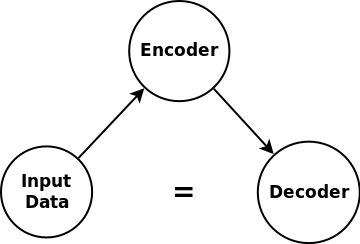
\includegraphics[width=0.5\textwidth]{pictures/figures/AE.png}
    \caption{Abstract structure of Auto-encoder}
    \label{fig:AE}
\end{figure}

To describe AE, let $\vec{x} = \{x_1, ..., x_n\} \in \mathbb{R}^n$ be an input, $\vec{e} = \{e_1, ..., e_m\} \in \mathbb{R}^m$ be an output from an encoder layer, and $\vec{d} = \{d_1, ..., d_n\} \in \mathbb{R}^n$ be an output from a decoder layer. For transform matrix, let $\bold{u}: \mathbb{R}^n \rightarrow \mathbb{R}^m$ be a transform matrix for an encode layer, $\bold{v}: \mathbb{R}^m \rightarrow \mathbb{R}^n$ be a transform matrix for a decode layer. Usually AE uses a sigmoid as an activation function. Figure \ref{fig:basic_AE} describes AE.

\begin{figure}[t!]
    \centering
    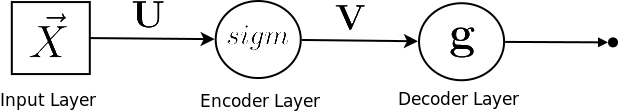
\includegraphics[width=0.5\textwidth]{pictures/figures/basic_AE.png}
    \caption{Basic Auto-encoder}
    \label{fig:basic_AE}
\end{figure}

The output of encoder is
$$\vec{e} = \bold{f}(\vec{X}\bold{U})$$
where $\bold{f}$ is the activation function for encoder layer. It is usually a sigmoid function.

The output of decoder is
$$\vec{d} = \bold{g}(\vec{E}\bold{V})$$
where $\bold{g}$ is the activation function for decoder layer. It is usually a sigmoid or a linear function.

The purpose of AE copies the input as the output. Therefore, the error function is calculated by
$$E(\vec{x}, \vec{d}) = E(\vec{x}, \bold{g}(\vec{E}\bold{V})) = E(\vec{x}, \bold{g}(\bold{f}(\vec{x}\bold{u}+\vec{b_e})\bold{v}+\vec{b_d}))$$
Where $\vec{b_e} = \{b_{e1}, ..., b_{em}\} \in \mathbb{R}^m$ is the bias for the encoder layer and $\vec{b_d} = \{b_{d1}, ..., b_{dm}\} \in \mathbb{R}^n$ is the bias for the decoder layer.

AE seems not useful because it only tries to copy inputs. However, AE is usually used with other neural network that uses data from an encoder layer of AE, not from a decoder layer. Making values of an input and a decoder output similar guarantees that a result from an encode layer contains all information of an input. It means that AE can represent the same information of an input data in different dimension. When the dimension of an encoder is higher than the dimension of an input, it is called an overcomplete Auto-encoder. When the dimension of an encoder is lower than the dimension of an input, it is called an undercomplete Auto-encoder.

On this paper and experiment, an undercomplete AE is used for reducing an input dimension. An undercomplete AE is often compared with principal components analysis (PCA) because both methods reduce dimensions. The paper \cite{hinton2006reducing} compares undercomplete AE and PCA. The result on the paper is that an undercomplete AE could keep more information than PCA. It means that reducing data to low dimension by an undercomplete AE gives better performance. However, training AE takes long time than computing information gained from PCA.

% When an auto-encoder is trained, it has two layers: an encode and a decode. The encode layer receives inputs and passes outputs in lower dimension data to a decode layer. The decode layer recovers the dimension to the input data dimension from the output of the encode layer. The error of an auto-encoder is measured by difference between the input data and the output from the decode layer. In other words, the encoder layer compresses the input data and the decoder layer decompresses data from the encoder layer that should be similar as the original input data. That methods guarantees that the data from the encoder layer keeps almost all properties of the input data in lower dimension. That is the reason why the output data from the decode layer is similar as the original input data. In mathematics, the relationship between an encoder and a decoder layer is similar as an inverse matrix of each other.


\subsubsection{Multilayer Auto-encoder}\label{subsubsec:MAE}
	Sometimes AE is designed with multiple encoder and decoder layers to reduce dimension. Figure \ref{fig:MAE} shows multilayer auto-encoder (MAE). However, it is difficult to find all the weights of encoders and decoders in MAE because all weights are initialized with random numbers and it makes difficult to find optimized weights \cite{zaremba2014recurrent}. So if the initial weights are close to optimized weights, training algorithm gradient descent can find optimized weights. The paper \cite{zaremba2014recurrent} shows "pretraining" method to initialize good weights.

\begin{figure}[t!]
    \centering
    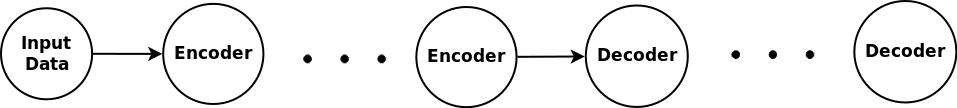
\includegraphics[width=0.75\textwidth]{pictures/figures/MAE.png}
    \caption{Multilayer Auto-encoder}
    \label{fig:MAE}
\end{figure}

\begin{figure}[t!]
    \centering
    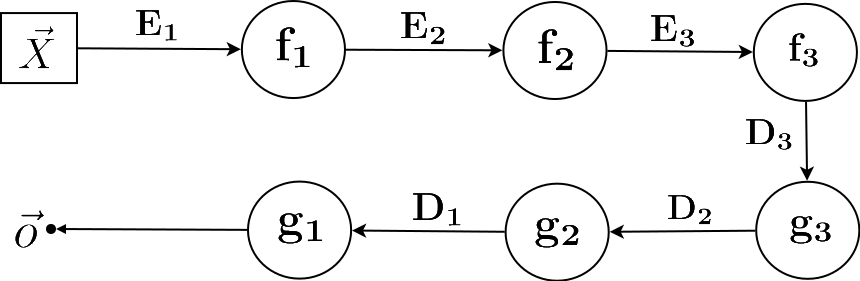
\includegraphics[width=0.75\textwidth]{pictures/figures/example_MAE.png}
    \caption{Multilayer Auto-encoder Example}
    \label{fig:example_MAE}
\end{figure}

	Pretraining is to train each layer separately before training the whole layers. For example, Figure \ref{fig:example_MAE} has three encoder and decoder layers. Let $\vec{x} \in \mathbb{R}^n$ be an input vector, $\bold{e_1}: \mathbb{R}^n \rightarrow \mathbb{R}^m$ be a transform matrix for the first encoder layer, $\bold{e_2}: \mathbb{R}^m \rightarrow \mathbb{R}^l$ be a transform matrix for the second encoder layer, $\bold{e_3}: \mathbb{R}^l \rightarrow \mathbb{R}^k$ be a transform matrix for the third encoder layer, $\bold{d_1}: \mathbb{R}^m \rightarrow \mathbb{R}^n$ be a transform matrix for the first decoder layer, $\bold{d_2}: \mathbb{R}^l \rightarrow \mathbb{R}^m$ be a transform matrix for the second decoder layer, $\bold{d_3}: \mathbb{R}^k \rightarrow \mathbb{R}^l$ be a transform matrix for the third decoder layer, and $\vec{o} \in \mathbb{R}^n$ be an output vector.

\begin{figure}[t!]
    \centering
    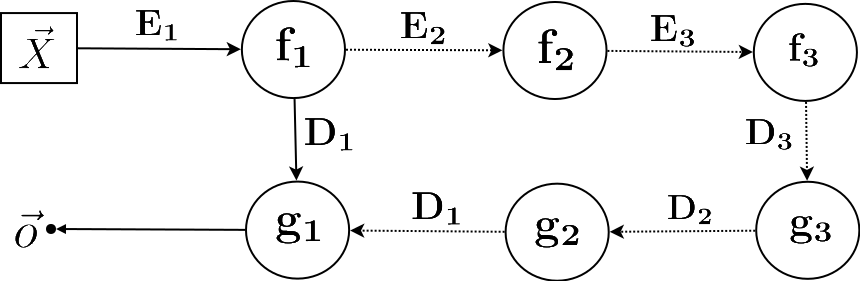
\includegraphics[width=0.3\textwidth]{pictures/figures/train_MAE1.png}
    \caption{Pretraining First Step}
    \label{fig:train_MAE1}
\end{figure}

\begin{figure}[t!]
    \centering
    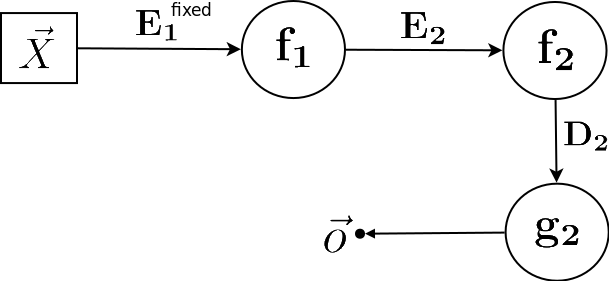
\includegraphics[width=0.5\textwidth]{pictures/figures/train_MAE2.png}
    \caption{Pretraining Second Step}
    \label{fig:train_MAE2}
\end{figure}

\begin{figure}[t!]
    \centering
    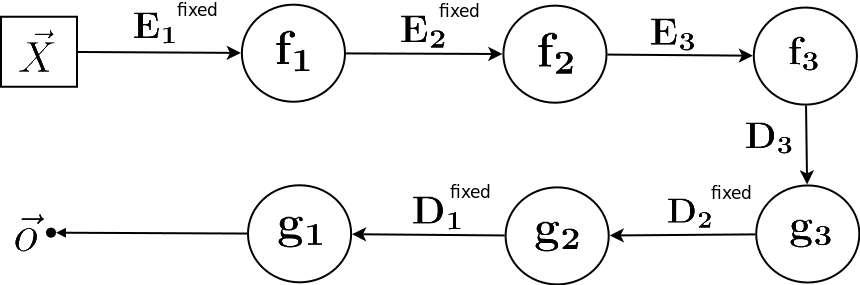
\includegraphics[width=0.75\textwidth]{pictures/figures/train_MAE3.png}
    \caption{Pretraining Thrid Step}
    \label{fig:train_MAE3}
\end{figure}

	In this case, pretraining has three steps because it has three encoder and decoder layers. Figure \ref{fig:train_MAE1} shows train of first encoder and decoder layer. While the first encoder and decoder layer are trained, the rest of encoders and decoders are ignored. So an error function is
$$E(\vec{x}, \bold{g_1}(\bold{f_1}(\vec{X}\bold{E_1})\bold{D_1}))$$
Figure \ref{fig:train_MAE2} shows the training of the second encoder and decoder layer. While the second encoder and decoder layer are trained, the transform matrix $\bold{e_1}$ is fixed because the transform matrix $\bold{e_1}$ is to create input for second layer encoder. So an error function is
$$E(\bold{f_1}(\vec{X}\bold{E_1^{fixed}}), \bold{g_2}(\bold{f_2}(\bold{f_1}(\vec{X}\bold{E_1^{fixed}})\bold{E_2})\bold{D_2}))$$
The last step is Figure \ref{fig:train_MAE3} and it trains the third encoder and decoder. During the training, the first and the second encoder weights are fixed. So an error function is
$$E(\bold{f_2}(\bold{f_1}(\vec{X}\bold{E_1^{fixed}})\bold{E_2^{fixed}}), \bold{g_3}(\bold{f_3}(\bold{f_2}(\bold{f_1}(\vec{X}\bold{E_1^{fixed}})\bold{E_2^{fixed}})\bold{E_3})\bold{D_3}))$$

	After finishing pretraining step, all weights are close enough to optimal weights for training algorithm to find the optimized answer when it trains the whole neural network. So an error function training the whole network is
$$E(\vec{x}, \bold{g_1}(\bold{g_2}(\bold{g_3}(\bold{f_3}(\bold{f_2}(\bold{f_1}(\vec{X}\bold{E_1})\bold{E_2})\bold{E_3})\bold{D_3})\bold{D_2})\bold{D_1}))$$


\section{Deep Learning Libraries}\label{sec:DLL}
This section introduces three popular libraries for deep learning.

\subsection{Tensorflow}
Tensorflow \footnote{\url{https://www.tensorflow.org/}} is an open source software library for numerical computation using data flow graphs. The biggest difference from other libraries is that Tensorflow treats all operator as a node. For example, multiplication, addition, or sigmoid function are treated as a node.  This helps developers to intuitively build neural network. Another strength is a TensorBoard. A TensorBoard is a tool for Tensorflow to visualize neural networks built in Tensorflow. Developers can also review how neural networks are trained from TensorBoard because TensorBoard visualizes logs to track all parameters while neural networks are trained.

The most famous example of Tensorflow is AlphaGo \footnote{\url{https://cloudplatform.googleblog.com/2016/05/Google-supercharges-machine-learning-tasks-with-custom-chip.html}}. Google engineer teams built AlphaGo with Tensorflow and the AlphaGo runs on Tensor Processing Unit (TPU).


\subsection{Theano}
Theano \footnote{\url{http://deeplearning.net/software/theano/}} is a Python library for machine learning. It integrates with Numpy and dynamically generates C code. Theano has many defined computations (called Op) and Theano allows to extend custom Ops written in C code.

Theano has more example codes and more stable than Tensorflow. This is because Tensorflow is newer than Theano and APIs of Tensorlfow keep changing. For example, many APIs in Tensorflow 1.x have different interfaces compared to APIs in Tensorflow 0.x.


\subsection{DL4J}
DL4J \footnote{\url{https://deeplearning4j.org/}} is open source, distributed deep-learning library for Java and Scala under the Apache 2.0 license. To compare with other deep learning libraries, DL4J can easily interact with Hadoop and Spark so neural networks built in DL4J can be used for big data.


\section{Machine Learning with Driving Data}\label{sec:MLDD}

% ####################################################################################################################################
\chapter{Data Set}\label{chap:dataset}
% ####################################################################################################################################

Data was collected in the high-fidelity simulator \cite{lee2017learning} of the Center for Injury Research Prevention Studies at the \textit{Children's Hospital of Philadelphia} (CHOP). The driving simulator provides an environment similar to real driving to test users. It has a 160 degree front view, rear-view, left side, and right side mirror images. It also features a full car chassis with active pedals, steering wheel, and a full dashboard with even audio equipment.

The experiments on this paper use 16 traces from 4 drivers: 2 people were expert drivers and 2 people were inexpert drivers. Each person drove four different tracks and each track represents different traffic situations and interactions with other vehicles. Each track has multiple instances of three scenarios that have been found to result in a high likelihood of crashing for 16-18 year- old teen drivers driving alone or with a peer passenger according to the NMVCCS (National Motor Vehicle Crash Causation Survey): 1) turning into opposite directions (turning left), 2) right roadside departure, and 3) rear-end events \cite{mcdonald2012using}. Thus, this results on a dataset that contains 8 traces of expert drivers, and 8 traces of inexpert drivers.

The simulator records 100 features which include car status: velocity, steer, Brake, throttle and etc. and include environment status features such as the current speed limit, whether the driver is instructed to make the next left or right turn, etc. These data is collected at 60Hz. The traces vary in length from 26298 to 51295, with an average of 33224.6875 instances. The specific lengths of each trace are shown on Table \ref{tbl:traces}

In this paper, we used two versions of the collected data set. A first version ({\em raw dataset}) contains 98 of the 100 features collected by the driving simulator (the two features that are removed are time stamps). A second version ({\em filtered dataset}) contains only 23 features. These 23 features were manually selected as are those that are most important for the classification task at hand. Reducing size of features helps save time to train neural network.

\begin{table}[!t]
\centering
\caption{Length of each of the traces used in our experiments.}
\label{tbl:traces}
\begin{tabular}{|l|l|l|l|}
\hline
{\em Trace}   & {\em Driver}    & {\em Track}  & {\em Length} \\ \hline
Trace0  & Expert0   & Track0 & 50029  \\
Trace1  & Expert0   & Track1 & 26375  \\
Trace2  & Expert0   & Track2 & 29629  \\
Trace3  & Expert0   & Track3 & 26298  \\
Trace4  & Expert1   & Track0 & 51295  \\
Trace5  & Expert1   & Track1 & 26674  \\
Trace6  & Expert1   & Track2 & 29680  \\
Trace7  & Expert1   & Track3 & 27075  \\
Trace8  & Inexpert0 & Track0 & 49691  \\
Trace9  & Inexpert0 & Track1 & 30058  \\
Trace10 & Inexpert0 & Track2 & 26441  \\
Trace11 & Inexpert0 & Track3 & 27373  \\
Trace12 & Inexpert1 & Track0 & 47658  \\
Trace13 & Inexpert1 & Track1 & 29380  \\
Trace14 & Inexpert1 & Track2 & 26684  \\
Trace15 & Inexpert1 & Track3 & 27255  \\ \hline
\end{tabular}
\end{table}


% ####################################################################################################################################
\chapter{Technical Approach}\label{chap:tech_approach}
% ####################################################################################################################################

This chapter covers technical methods for experiments on the paper and also introduces three different neural network used for the experiments.


\section{Cross Validation}
Cross validation (CV) is used to validate model when data is not enough \cite{Goodfellow-et-al-2016}. CV divides data set to $K$ folds then applies $i$th fold as test set and other folds as train set to target model. Experiments on the paper use 16 traces but it is not enough to train neural network. CV can be used to validate neural network model and compare performance of three different models. The 16 traces dataset is divided to 4 folds. Each folds contain two traces from expert and two traces from inexpert. The neural networks are trained four times with different train (3 folds) and test (1 fold) set. Figure \ref{fig:CV} shows four folds cross validation. Red color is the fold for testing and other folds are for training.

\begin{figure}[t!]
    \centering
    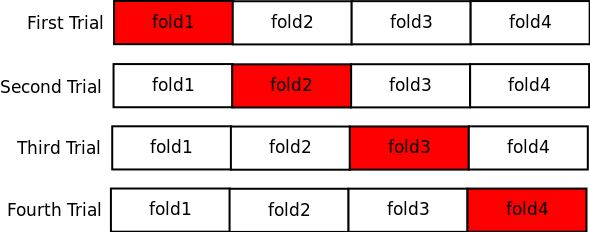
\includegraphics[width=0.7\textwidth]{pictures/figures/CV.png}
    \caption{Cross Validation}
    \label{fig:CV}
\end{figure}


\section{LSTM}
The LSTM neural network is used on three different neural network models to classify expert or inexpert drivers because the data has time domain and LSTM gives good performance for serial data. On the paper, LSTM neural network is built with 16, 32, 64, 128, and 256 hidden neurons. The output from LSTM is sent to the output layer which has two neurons. By using a softmax, the output from two neurons is classified. If it has [0, 1], it is classified to experts. Otherwise, it is classified to inexperts.

Figure \ref{fig:exp_NN1} shows first neural network model ({\em first model}) on the paper. Its input is {\em filtered dataset} which has 23 chosen features. The {\em filtered dataset} is feed directly to LSTM then the result is passed to the output layer.

\begin{figure}[t!]
    \centering
    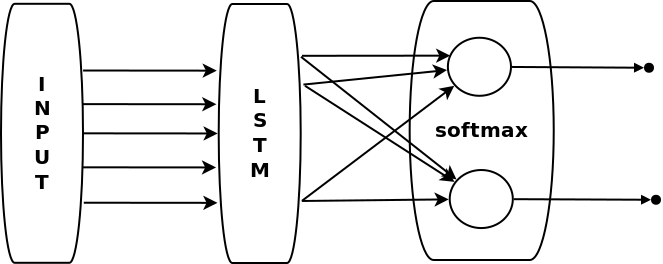
\includegraphics[width=0.7\textwidth]{pictures/figures/exp_NN1.png}
    \caption{First experiment NN}
    \label{fig:exp_NN1}
\end{figure}


\section{Auto-encoder}
The {\em raw dataset} has 98 features and it takes too much time to train nerual network if all 98 features are used. AE can solve the problem by reducing dimensions.

\subsection{Single layer Auto-encoder}
Figure \ref{fig:exp_NN2} shows the second neural network model ({\em second model}) on the paper. The {\em second model} is added by one AE layer from {\em first model}. The purpose of the AE layer is to reduce 98 features to 25 features on {\em raw dataset}. Notice that the figure has an encoder only because after training AE, only an encoder is used to reduce dimensions. The output from the encoder is passed to LSTM.

\begin{figure}[t!]
    \centering
    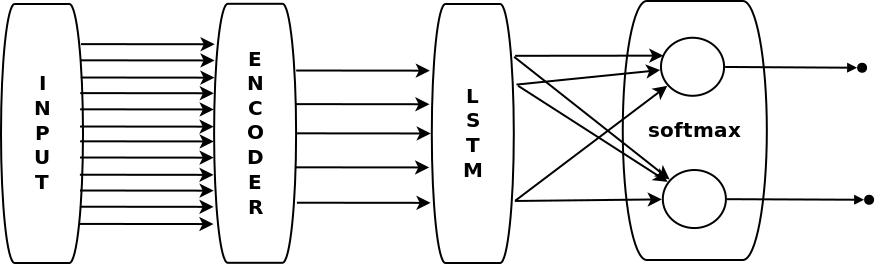
\includegraphics[width=0.8\textwidth]{pictures/figures/exp_NN2.png}
    \caption{Second experiment NN}
    \label{fig:exp_NN2}
\end{figure}


\subsection{Multiple layer Auto-encoder}
Figure \ref{fig:exp_NN3} shows third neural network model ({\em third model}) on the paper. To compare the performance between a single layer AE and multiple layer AE, the {\em third model} has three layers of AE.  THe first AE reduces 98 dimensions to 75 dimensions, the second AE reduces 75 dimensions to 50 dimensions and the last AE reduces 50 dimensions to 25 dimensions. The figure describes it with three encoder layers.

\begin{figure}[t!]
    \centering
    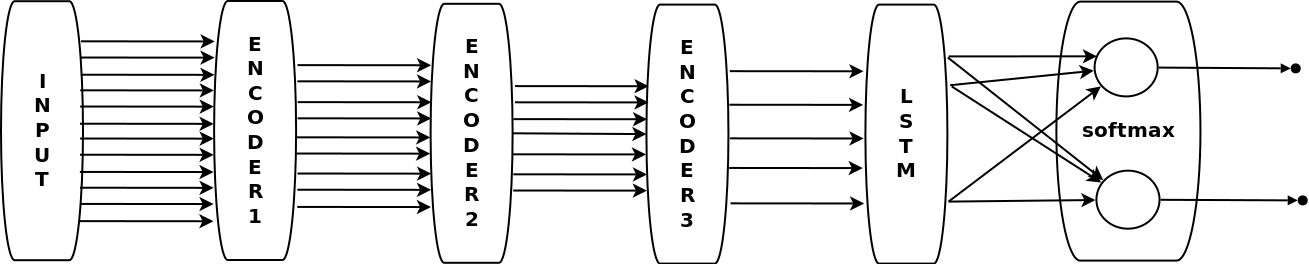
\includegraphics[width=\textwidth]{pictures/figures/exp_NN3.png}
    \caption{Third experiment NN}
    \label{fig:exp_NN3}
\end{figure}


\section{Sampling}
The simulator records 60 samples per second. It is too often recorded. The dataset is re-sampled by three different periods: 1 over 10, 1 over 20, and 1 over 50. When it is re-sampled, three methods are used. The first method {\em last} chooses the last sample of period, the second method {\em mean} computes mean of data in period, and the third method {\em gaussian} applies Gaussian filter. For the third method, window size is 11, 21, and 51 for each periods which are one more greater than periods. Below example explains how to re-sample data.

\begin{table}[!t]
\centering
\caption{Example Data}
\label{tbl:example_data}
\begin{tabular}{|l|}
\hline
Example Data \\ \hline
1            \\
2            \\
3            \\
4            \\
5            \\
6            \\
7            \\
8            \\
9            \\
10           \\
11           \\
12           \\
13           \\
14           \\
15           \\
16           \\
17           \\
18           \\
19           \\
20           \\
21           \\ \hline
\end{tabular}
\end{table}

\begin{table}[!t]
\centering
\caption{Result of Re-Sampled Data}
\label{tbl:result_resample}
\begin{tabular}{|l|l|l|}
\hline
{\em last} & {\em mean} & {\em gaussian}    \\ \hline
10   & 5.5  & 5.999996063 \\
20   & 15.5 & 15.9999895  \\ \hline
\end{tabular}
\end{table}

Table \ref{tbl:example_data} shows example data and Table \ref{tbl:result_resample} shows result of re-sampled data by 1 over 10 from each methods. To explain three re-sample methods, let {\em first period} be $(1, 2, 3, 4, 5, 6, 7, 8, 9, 10)$ and {\em second period} be $(11, 12, 13, 14, 15, 16, 17, 18, 19, 20)$. The {\em last} method takes last sample from each periods. The result from {\em last} method is $(10, 20)$ because last sample from {\em first period} is $10$ and last sample from {\em second period} is $20$. The {\em mean} method computes mean of samples in a period. The result from {\em mean} is $(5.5, 15.5)$ because mean of {\em first period} is $5.5$ and mean of {\em second period} is $15.5$.

Before explaining {\em gaussian} method, Gaussian filter should be defined. The filter size is greater than sampling size by 1. In this case, Gaussian filter size is 11 because sampling size is 10. Below equation is Gaussian equation and used to make Gaussian filter.
$$g(x) = \frac{1}{\sqrt{2\pi}\sigma}e^{-\frac{x^2}{2\sigma^2}}$$
where $\sigma = \frac{filter\_size-1}{6.0}$ because the sum of filter closes to 1 with the $\sigma$. With filter size 11, $\sigma$ is $1.667$.

\begin{table}[!t]
\centering
\caption{Gaussian Filter (size=11, $\sigma$=1.667)}
\label{tbl:gaussian_filter}
\begin{tabular}{|l|l|}
\hline
x  & Gaussian Value \\ \hline
5  & 0.00266126292  \\
4  & 0.01344760189  \\
3  & 0.04740846466  \\
2  & 0.1166060072   \\
1  & 0.2000967085   \\
0  & 0.2395592537   \\
-1 & 0.2000967085   \\
-2 & 0.1166060072   \\
-3 & 0.04740846466  \\
-4 & 0.01344760189  \\
-5 & 0.00266126292  \\ \hline
\end{tabular}
\end{table}

\begin{table}[!t]
\centering
\caption{First Period applied by Gaussian Filter}
\label{tbl:first_period}
\begin{tabular}{|l|ll|}
\hline
First Period & \multicolumn{1}{l|}{Gaussian Value} & Filtered Value \\ \hline
1            & \multicolumn{1}{l|}{0.00266126292}  & 0.00266126292  \\
2            & \multicolumn{1}{l|}{0.01344760189}  & 0.02689520378  \\
3            & \multicolumn{1}{l|}{0.04740846466}  & 0.142225394    \\
4            & \multicolumn{1}{l|}{0.1166060072}   & 0.4664240287   \\
5            & \multicolumn{1}{l|}{0.2000967085}   & 1.000483542    \\
6            & \multicolumn{1}{l|}{0.2395592537}   & 1.437355522    \\
7            & \multicolumn{1}{l|}{0.2000967085}   & 1.400676959    \\
8            & \multicolumn{1}{l|}{0.1166060072}   & 0.9328480573   \\
9            & \multicolumn{1}{l|}{0.04740846466}  & 0.4266761819   \\
10           & \multicolumn{1}{l|}{0.01344760189}  & 0.1344760189   \\
11           & \multicolumn{1}{l|}{0.00266126292}  & 0.02927389212  \\ \hline
\multicolumn{2}{|l|}{Sum}                          & 5.999996063    \\ \hline
\end{tabular}
\end{table}

\begin{table}[!t]
\centering
\caption{Second Period applied by Gaussian Filter}
\label{tbl:second_period}
\begin{tabular}{|l|l|l|}
\hline
First Period & Gaussian Value & Filtered Value \\ \hline
11           & 0.00266126292  & 0.02927389212  \\
12           & 0.01344760189  & 0.1613712227   \\
13           & 0.04740846466  & 0.6163100406   \\
14           & 0.1166060072   & 1.6324841      \\
15           & 0.2000967085   & 3.001450627    \\
16           & 0.2395592537   & 3.832948059    \\
17           & 0.2000967085   & 3.401644044    \\
18           & 0.1166060072   & 2.098908129    \\
19           & 0.04740846466  & 0.9007608285   \\
20           & 0.01344760189  & 0.2689520378   \\
21           & 0.00266126292  & 0.05588652132  \\ \hline
\multicolumn{2}{|l|}{Sum}     & 15.9999895     \\ \hline
\end{tabular}
\end{table}

Table \ref{tbl:gaussian_filter} shows size 11 Gaussian filter with $\sigma=1.667$. Re-sampling example data by the Gaussian filter is just multiplication between filter and data. Table \ref{tbl:first_period} shows Gaussian filtered values for {\em first period}. The re-sampled value from {\em first period} is sum of Gaussian filtered values. That is 5.999996063. Table \ref{tbl:second_period} shows Gaussian filtered values for {\em second period}. The re-sampled value is 15.9999895.


\section{Standardization}
After feeding re-sampled data to three neural network models, the data is standardized: mean is 0, standard deviation is 1. CV is used for all experiments. Therefore, standardization is done in a training set without a testing set in CV. This is because the testing set should be hidden until final neural network models are applied on that. The testing set refers mean and standard deviation from the training set to standardize.


% ####################################################################################################################################
\chapter{Experiment Result}\label{chap:result}
% ####################################################################################################################################
This chapter summarizes results from all experiments. Experiments are divided to two parts: 1) experiments with {\em filtered dataset} 2) experiments with {\em raw dataset}. First part of experiments used {\em first model} which only has LSTM. Each experiments used 5 different number of neurons: 16, 32, 64, 128, and 256. Second part of experiments used {\em second model} which has SAE and {\em third model} which has MAE then compared result of three models.

\section{Experiments with {\em filtered dataset}}
The first part of experiments used {\em filtered dataset} which has chosen 23 features. The dataset was re-sampled by 1 over 10, 1 over 20, and 1 over 50 with three different methods: {\em last}, {\em mean}, and {\em gaussian} so it was 9 different re-sampled datasets.

\subsection{Resample 1 over 50}
This subsection compares results from experiments with re-sampled {\em filtered dataset} by 1 over 50. Figure \ref{fig:filter_1_50} shows average accuracy of four tests on different number of neurons in LSTM hidden layer. Table \ref{tbl:last_1_50}, Table \ref{tbl:mean_1_50}, and Table \ref{tbl:gaussian_1_50} show detail result from {\em last} method, {\em mean} method, and {\em gaussian} method respectively. Table \ref{tbl:last_1_50_time}, Table \ref{tbl:mean_1_50_time}, and Table \ref{tbl:gaussian_1_50_time} show how much time experiments took from {\em last} method, {\em mean}method, and {\em gaussian} method respectively.

The best performance was from {\em last} method with 16 number of neurons. The accuracy of this was 0.59375 (59.375\%). The worst performance was from {\em gaussian} method with 64 number of neurons. It was 0.40625 (40.625\%). Many accuracy were below 0.5 (50\%) and total average accuracy is 0.492708 (49.2708\%). The experiments with 1 over 50 re-sampled data took short time than experiments with 1 over 20 and 1 over 10 re-sampled data on later of this chapter.

\begin{figure}[t!]
    \centering
    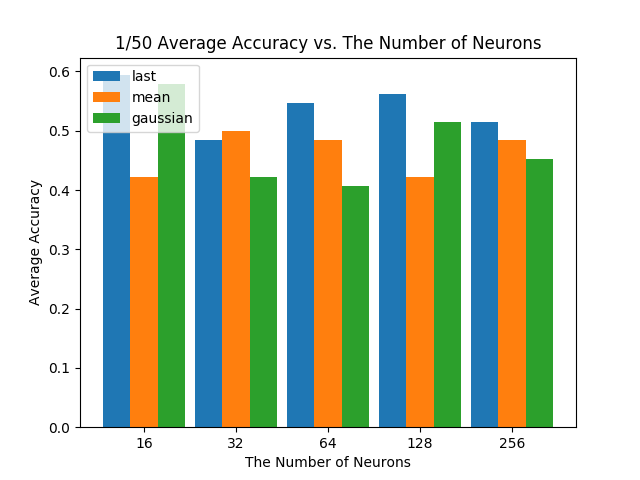
\includegraphics[width=0.75\textwidth]{pictures/result_pictures/filtered_1_50_result.png}
    \caption{Result of 1 over 50 from {\em filtered dataset}}
    \label{fig:filter_1_50}
\end{figure}

\begin{table}[!t]
\centering
\caption{{\em last} method on 1 over 50 Re-sampled {\em filtered dataset}}
\label{tbl:last_1_50}
\begin{tabular}{|c|c|c|c|c|c|c|}
\hline
\multirow{2}{*}{Test} & \multirow{2}{*}{CV} & \multicolumn{5}{c|}{The number of neurans}                              \\ \cline{3-7}
                      &                     & 16           & 32           & 64           & 128         & 256          \\ \hline
\multirow{4}{*}{1}    & 1                   & 1            & 0.5          & 0.5          & 0.75        & 0.25         \\ \cline{2-7}
                      & 2                   & 0.25         & 0.25         & 0.5          & 0.25        & 0.75         \\ \cline{2-7}
                      & 3                   & 0.75         & 0.25         & 0.25         & 0.75        & 0.75         \\ \cline{2-7}
                      & 4                   & 0.75         & 0.75         & 0.5          & 0.75        & 0.75         \\ \hline
\multirow{4}{*}{2}    & 1                   & 0.5          & 0            & 0.75         & 0.75        & 0.5          \\ \cline{2-7}
                      & 2                   & 0.25         & 0.25         & 0.5          & 0.5         & 0.25         \\ \cline{2-7}
                      & 3                   & 0.75         & 0.25         & 0.25         & 0.5         & 1            \\ \cline{2-7}
                      & 4                   & 0.5          & 0.5          & 0.75         & 0.5         & 0.5          \\ \hline
\multirow{4}{*}{3}    & 1                   & 0.5          & 0.75         & 0.5          & 0.75        & 0            \\ \cline{2-7}
                      & 2                   & 0.5          & 0.5          & 0.75         & 0.75        & 0.5          \\ \cline{2-7}
                      & 3                   & 0.5          & 0.5          & 0.25         & 0.25        & 0.5          \\ \cline{2-7}
                      & 4                   & 0.75         & 0.75         & 0.75         & 0.25        & 0.5          \\ \hline
\multirow{4}{*}{4}    & 1                   & 0.75         & 0.5          & 0.75         & 0.75        & 0.5          \\ \cline{2-7}
                      & 2                   & 0.25         & 0.5          & 0.5          & 0.25        & 0.75         \\ \cline{2-7}
                      & 3                   & 0.5          & 0.75         & 0.75         & 0.75        & 0.25         \\ \cline{2-7}
                      & 4                   & 1            & 0.75         & 0.5          & 0.5         & 0.5          \\ \hline
\multicolumn{2}{|c|}{Mean}                  & 0.59375      & 0.484375     & 0.546875     & 0.5625      & 0.515625     \\ \hline
\multicolumn{2}{|c|}{Std}                   & 0.1983000672 & 0.2536196299 & 0.1547847968 & 0.249478623 & 0.2452677109 \\ \hline
\end{tabular}
\end{table}

\begin{table}[!t]
\centering
\caption{{\em mean} method on 1 over 50 Re-sampled {\em filtered dataset}}
\label{tbl:mean_1_50}
\begin{tabular}{|c|c|c|c|c|c|c|}
\hline
\multirow{2}{*}{Test} & \multirow{2}{*}{CV} & \multicolumn{5}{c|}{The number of neurans}                             \\ \cline{3-7}
                      &                     & 16          & 32           & 64          & 128          & 256          \\ \hline
\multirow{4}{*}{1}    & 1                   & 0.5         & 0.5          & 0           & 0.25         & 0.25         \\ \cline{2-7}
                      & 2                   & 0.5         & 0.5          & 0.25        & 0.5          & 0.5          \\ \cline{2-7}
                      & 3                   & 0           & 0.75         & 0.5         & 0.25         & 0.75         \\ \cline{2-7}
                      & 4                   & 0           & 0.5          & 0.25        & 0.25         & 0.25         \\ \hline
\multirow{4}{*}{2}    & 1                   & 0.5         & 0.5          & 0.5         & 0.5          & 0            \\ \cline{2-7}
                      & 2                   & 0.25        & 0.25         & 0.5         & 0.75         & 0.75         \\ \cline{2-7}
                      & 3                   & 0.5         & 0.5          & 0.75        & 0.5          & 0.25         \\ \cline{2-7}
                      & 4                   & 0.25        & 0.25         & 0.5         & 0.75         & 0.25         \\ \hline
\multirow{4}{*}{3}    & 1                   & 0.5         & 0.25         & 0.5         & 0.5          & 0.5          \\ \cline{2-7}
                      & 2                   & 0.25        & 0.5          & 0.75        & 0.5          & 0.25         \\ \cline{2-7}
                      & 3                   & 0.5         & 0.75         & 0.5         & 0.25         & 0.5          \\ \cline{2-7}
                      & 4                   & 0.75        & 0.5          & 0.5         & 0.75         & 0.5          \\ \hline
\multirow{4}{*}{4}    & 1                   & 0.5         & 0.5          & 0.75        & 0.25         & 1            \\ \cline{2-7}
                      & 2                   & 0.75        & 0.75         & 0.5         & 0.25         & 0.5          \\ \cline{2-7}
                      & 3                   & 0.5         & 0.25         & 0.25        & 0.25         & 0.75         \\ \cline{2-7}
                      & 4                   & 0.5         & 0.75         & 0.75        & 0.25         & 0.75         \\ \hline
\multicolumn{2}{|c|}{Mean}                  & 0.421875    & 0.5          & 0.484375    & 0.421875     & 0.484375     \\ \hline
\multicolumn{2}{|c|}{Std}                   & 0.218303115 & 0.1825741858 & 0.213478141 & 0.1983000672 & 0.2656556355 \\ \hline
\end{tabular}
\end{table}

\begin{table}[!t]
\centering
\caption{{\em gaussian} method on 1 over 50 Re-sampled {\em filtered dataset}}
\label{tbl:gaussian_1_50}
\begin{tabular}{|c|c|c|c|c|c|c|}
\hline
\multirow{2}{*}{Test} & \multirow{2}{*}{CV} & \multicolumn{5}{c|}{The number of neurans}                              \\ \cline{3-7}
                      &                     & 16           & 32           & 64           & 128         & 256          \\ \hline
\multirow{4}{*}{1}    & 1                   & 0.25         & 0.5          & 0.5          & 0.25        & 0.25         \\ \cline{2-7}
                      & 2                   & 0.75         & 0.75         & 0.25         & 0.75        & 0.5          \\ \cline{2-7}
                      & 3                   & 0.25         & 1            & 0.25         & 0.5         & 0.25         \\ \cline{2-7}
                      & 4                   & 0.5          & 0.25         & 0.25         & 0.5         & 0.75         \\ \hline
\multirow{4}{*}{2}    & 1                   & 0.75         & 0.25         & 0.5          & 0.5         & 0.5          \\ \cline{2-7}
                      & 2                   & 0.5          & 0.75         & 0.25         & 0.5         & 0.25         \\ \cline{2-7}
                      & 3                   & 0.5          & 0.5          & 0.5          & 0           & 0.25         \\ \cline{2-7}
                      & 4                   & 0.75         & 0            & 0.75         & 0.75        & 1            \\ \hline
\multirow{4}{*}{3}    & 1                   & 0.75         & 0.5          & 0.5          & 0.5         & 0.25         \\ \cline{2-7}
                      & 2                   & 0.75         & 0.25         & 0.5          & 0           & 0.5          \\ \cline{2-7}
                      & 3                   & 0.75         & 0.25         & 0.5          & 0.75        & 0.75         \\ \cline{2-7}
                      & 4                   & 0.5          & 0.25         & 0.25         & 0.75        & 0.75         \\ \hline
\multirow{4}{*}{4}    & 1                   & 0.75         & 0.5          & 0.5          & 0.75        & 0.25         \\ \cline{2-7}
                      & 2                   & 0.25         & 0.5          & 0.25         & 0.5         & 0.25         \\ \cline{2-7}
                      & 3                   & 0.75         & 0.25         & 0.5          & 0.75        & 0.5          \\ \cline{2-7}
                      & 4                   & 0.5          & 0.25         & 0.25         & 0.5         & 0.25         \\ \hline
\multicolumn{2}{|c|}{Mean}                  & 0.578125     & 0.421875     & 0.40625      & 0.515625    & 0.453125     \\ \hline
\multicolumn{2}{|c|}{Std}                   & 0.1983000672 & 0.2536196299 & 0.1547847968 & 0.249478623 & 0.2452677109 \\ \hline
\end{tabular}
\end{table}

\begin{table}[!t]
\centering
\caption{{\em last} Test Time with 1 over 50 Re-sampled {\em filtered dataset}}
\label{tbl:last_1_50_time}
\begin{tabular}{|c|c|c|c|c|c|}
\hline
\multirow{2}{*}{Test}      & \multicolumn{5}{c|}{The number of neurans}                                                                                                               \\ \cline{2-6}
                           & 16                           & 32                           & 64                           & 128                          & 256                          \\ \hline
1                          & 0:18:41                      & 0:20:07                      & 0:23:00                      & 0:39:32                      & 0:54:27                      \\ \hline
2                          & 0:16:28                      & 0:18:18                      & 0:22:19                      & 0:34:39                      & 0:47:47                      \\ \hline
3                          & 0:16:25                      & 0:18:17                      & 0:22:15                      & 0:34:38                      & 0:49:43                      \\ \hline
4                          & 0:16:36                      & 0:18:28                      & 0:23:19                      & 0:34:01                      & 0:53:42                      \\ \hline
\multicolumn{1}{|l|}{Mean} & \multicolumn{1}{l|}{0:17:03} & \multicolumn{1}{l|}{0:18:48} & \multicolumn{1}{l|}{0:22:43} & \multicolumn{1}{l|}{0:35:43} & \multicolumn{1}{l|}{0:51:25} \\ \hline
\end{tabular}
\end{table}

\begin{table}[!t]
\centering
\caption{{\em mean} Test Time with 1 over 50 Re-sampled {\em filtered dataset}}
\label{tbl:mean_1_50_time}
\begin{tabular}{|c|c|c|c|c|c|}
\hline
\multirow{2}{*}{Test}      & \multicolumn{5}{c|}{The number of neurans}                                                                                                               \\ \cline{2-6}
                           & 16                           & 32                           & 64                           & 128                          & 256                          \\ \hline
1                          & 0:18:33                      & 0:19:09                      & 0:23:59                      & 0:34:57                      & 0:51:25                      \\ \hline
2                          & 0:16:25                      & 0:17:16                      & 0:22:33                      & 0:35:32                      & 0:47:26                      \\ \hline
3                          & 0:16:48                      & 0:18:07                      & 0:22:46                      & 0:34:57                      & 0:52:14                      \\ \hline
4                          & 0:16:39                      & 0:18:36                      & 0:23:23                      & 0:36:05                      & 0:51:44                      \\ \hline
\multicolumn{1}{|l|}{Mean} & \multicolumn{1}{l|}{0:17:03} & \multicolumn{1}{l|}{0:18:48} & \multicolumn{1}{l|}{0:22:43} & \multicolumn{1}{l|}{0:35:43} & \multicolumn{1}{l|}{0:51:25} \\ \hline
\end{tabular}
\end{table}

\begin{table}[!t]
\centering
\caption{{\em gaussian} Test Time with 1 over 50 Re-sampled {\em filtered dataset}}
\label{tbl:gaussian_1_50_time}
\begin{tabular}{|c|c|c|c|c|c|}
\hline
\multirow{2}{*}{Test}      & \multicolumn{5}{c|}{The number of neurans}                                                                                                               \\ \cline{2-6}
                           & 16                           & 32                           & 64                           & 128                          & 256                          \\ \hline
1                          & 0:18:05                      & 0:18:33                      & 0:22:40                      & 0:37:31                      & 0:54:11                      \\ \hline
2                          & 0:16:24                      & 0:18:08                      & 0:22:19                      & 0:35:22                      & 0:48:40                      \\ \hline
3                          & 0:16:17                      & 0:18:00                      & 0:22:18                      & 0:35:12                      & 0:53:03                      \\ \hline
4                          & 0:16:28                      & 0:18:39                      & 0:22:33                      & 0:34:25                      & 0:54:57                      \\ \hline
\multicolumn{1}{|l|}{Mean} & \multicolumn{1}{l|}{0:16:49} & \multicolumn{1}{l|}{0:18:20} & \multicolumn{1}{l|}{0:22:28} & \multicolumn{1}{l|}{0:35:38} & \multicolumn{1}{l|}{0:52:43} \\ \hline
\end{tabular}
\end{table}


\subsection{Resample 1 over 20}
This subsection compares results from experiments with re-sampled {\em filtered dataset} by 1 over 20. Figure \ref{fig:filter_1_20} shows the average accuracy of four tests on different number of neurons in LSTM hidden layer. Table \ref{tbl:last_1_20}, Table \ref{tbl:mean_1_20}, and Table \ref{tbl:gaussian_1_20} show a detailed result from {\em last} method, {\em mean} method, and {\em gaussian} method respectively. Table \ref{tbl:last_1_20_time}, Table \ref{tbl:mean_1_20_time}, and Table \ref{tbl:gaussian_1_20_time} show how much time experiments took from {\em last} method, {\em mean}method, and {\em gaussian} method respectively.

The best performance was from {\em mean} method with 32 and 256 number of neurons. The accuracy of this was 0.59375 (59.375\%) as same as best performance from experiments with 1 over 50 re-sampled data. The worst performance was also from {\em mean} method with 128 number of neurons. It was 0.375 (37.5\%), which was worse than the worst performance from experiments with 1 over 50 re-sampled data. However, the total average was 0.515625 (51.5625\%) which was slightly higher than the total average 0.492708 (49.2708\%) from experiments with 1 over 50 re-sampled data because size of 1 over 20 re-sampled data is 2.5 times more than size of 1 over 50 re-sampled data. More amount of data also affected the test time. Even size of the data is 2.5 times more, the test time took more than 2.5 times than the test time from experiments with 1 over 50 re-sampled data.

\begin{figure}[t!]
    \centering
    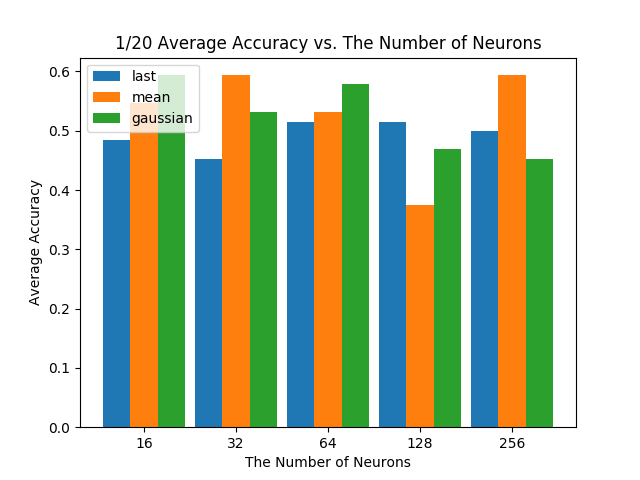
\includegraphics[width=0.75\textwidth]{pictures/result_pictures/filtered_1_20_result.png}
    \caption{Result of 1 over 20 from {\em filtered dataset}}
    \label{fig:filter_1_20}
\end{figure}

\begin{table}[!t]
\centering
\caption{{\em last} method on 1 over 20 Re-sampled {\em filtered dataset}}
\label{tbl:last_1_20}
\begin{tabular}{|c|c|c|c|c|c|c|}
\hline
\multirow{2}{*}{Test} & \multirow{2}{*}{CV} & \multicolumn{5}{c|}{The number of neurans}                             \\ \cline{3-7}
                      &                     & 16           & 32           & 64          & 128         & 256          \\ \hline
\multirow{4}{*}{1}    & 1                   & 0.75         & 0.5          & 0.25        & 0.5         & 0.5          \\ \cline{2-7}
                      & 2                   & 0.5          & 0.25         & 0.75        & 0.5         & 0.5          \\ \cline{2-7}
                      & 3                   & 0.5          & 0.25         & 0.5         & 0.5         & 0.25         \\ \cline{2-7}
                      & 4                   & 0.5          & 0.25         & 0.75        & 0.25        & 0.5          \\ \hline
\multirow{4}{*}{2}    & 1                   & 0.25         & 1            & 0.25        & 0.5         & 0            \\ \cline{2-7}
                      & 2                   & 0.5          & 0.25         & 0.5         & 0.5         & 0.75         \\ \cline{2-7}
                      & 3                   & 0.5          & 0.25         & 0.5         & 0.5         & 0.5          \\ \cline{2-7}
                      & 4                   & 0.5          & 0.5          & 0.25        & 0.25        & 0.25         \\ \hline
\multirow{4}{*}{3}    & 1                   & 0.25         & 0.75         & 0.5         & 0.5         & 0.5          \\ \cline{2-7}
                      & 2                   & 0.25         & 0            & 0.75        & 0.5         & 0.5          \\ \cline{2-7}
                      & 3                   & 0.5          & 0.5          & 0.5         & 0.75        & 0.75         \\ \cline{2-7}
                      & 4                   & 0.25         & 0.5          & 0.5         & 0.25        & 0.75         \\ \hline
\multirow{4}{*}{4}    & 1                   & 0.75         & 0.5          & 0.5         & 0.25        & 0.5          \\ \cline{2-7}
                      & 2                   & 0.25         & 0.75         & 1           & 0.75        & 0.25         \\ \cline{2-7}
                      & 3                   & 0.75         & 0.75         & 0.25        & 0.75        & 1            \\ \cline{2-7}
                      & 4                   & 0.75         & 0.25         & 0.5         & 1           & 0.5          \\ \hline
\multicolumn{2}{|c|}{Mean}                  & 0.484375     & 0.453125     & 0.515625    & 0.515625    & 0.5          \\ \hline
\multicolumn{2}{|c|}{Std}                   & 0.1929756029 & 0.2617051458 & 0.213478141 & 0.213478141 & 0.2415229458 \\ \hline
\end{tabular}
\end{table}

\begin{table}[!t]
\centering
\caption{{\em mean} method on 1 over 20 Re-sampled {\em filtered dataset}}
\label{tbl:mean_1_20}
\begin{tabular}{|c|c|c|c|c|c|c|}
\hline
\multirow{2}{*}{Test} & \multirow{2}{*}{CV} & \multicolumn{5}{c|}{The number of neurans}                           \\ \cline{3-7}
                      &                     & 16       & 32           & 64           & 128          & 256          \\ \hline
\multirow{4}{*}{1}    & 1                   & 0.5      & 0.5          & 0.5          & 0.25         & 0.75         \\ \cline{2-7}
                      & 2                   & 0.25     & 0.5          & 0.25         & 0            & 1            \\ \cline{2-7}
                      & 3                   & 0.75     & 0.25         & 0.75         & 0.25         & 0.25         \\ \cline{2-7}
                      & 4                   & 0.75     & 1            & 0.25         & 0.75         & 0.75         \\ \hline
\multirow{4}{*}{2}    & 1                   & 0.75     & 0.75         & 0.5          & 0.5          & 0.75         \\ \cline{2-7}
                      & 2                   & 0.75     & 0.25         & 0.5          & 0.25         & 0.5          \\ \cline{2-7}
                      & 3                   & 0.5      & 0.75         & 0.75         & 0.5          & 0.25         \\ \cline{2-7}
                      & 4                   & 0.5      & 0.5          & 0.75         & 0.5          & 0.75         \\ \hline
\multirow{4}{*}{3}    & 1                   & 0.5      & 0.75         & 0.5          & 0            & 0.5          \\ \cline{2-7}
                      & 2                   & 0.75     & 1            & 0.5          & 0.5          & 0.5          \\ \cline{2-7}
                      & 3                   & 0.25     & 0.25         & 0.5          & 0.5          & 0.5          \\ \cline{2-7}
                      & 4                   & 0.5      & 0.5          & 0.5          & 0.75         & 0.75         \\ \hline
\multirow{4}{*}{4}    & 1                   & 0.5      & 0.5          & 0.75         & 0.25         & 1            \\ \cline{2-7}
                      & 2                   & 0.25     & 1            & 0.5          & 0.75         & 0.5          \\ \cline{2-7}
                      & 3                   & 0.5      & 0.5          & 0.5          & 0            & 0.25         \\ \cline{2-7}
                      & 4                   & 0.75     & 0.5          & 0.5          & 0.25         & 0.5          \\ \hline
\multicolumn{2}{|c|}{Mean}                  & 0.546875 & 0.59375      & 0.53125      & 0.375        & 0.59375      \\ \hline
\multicolumn{2}{|c|}{Std}                   & 0.1875   & 0.2561737691 & 0.1547847968 & 0.2581988897 & 0.2393567769 \\ \hline
\end{tabular}
\end{table}

\begin{table}[!t]
\centering
\caption{{\em gaussian} method on 1 over 20 Re-sampled {\em filtered dataset}}
\label{tbl:gaussian_1_20}
\begin{tabular}{|c|c|c|c|c|c|c|}
\hline
\multirow{2}{*}{Test} & \multirow{2}{*}{CV} & \multicolumn{5}{c|}{The number of neurans}                               \\ \cline{3-7}
                      &                     & 16           & 32           & 64           & 128          & 256          \\ \hline
\multirow{4}{*}{1}    & 1                   & 0.5          & 0.5          & 0.5          & 0.5          & 0.5          \\ \cline{2-7}
                      & 2                   & 0.25         & 0.25         & 0.25         & 0.5          & 0.75         \\ \cline{2-7}
                      & 3                   & 0.75         & 1            & 0.75         & 0.25         & 0            \\ \cline{2-7}
                      & 4                   & 0.5          & 0.5          & 0.25         & 0.75         & 0.25         \\ \hline
\multirow{4}{*}{2}    & 1                   & 0.75         & 0.75         & 0.5          & 0.25         & 1            \\ \cline{2-7}
                      & 2                   & 1            & 0.75         & 0.75         & 0.75         & 0.25         \\ \cline{2-7}
                      & 3                   & 0.75         & 0.75         & 0.75         & 0.25         & 0.25         \\ \cline{2-7}
                      & 4                   & 0.75         & 0.25         & 1            & 0.5          & 0.25         \\ \hline
\multirow{4}{*}{3}    & 1                   & 0.75         & 0.75         & 0.75         & 0.5          & 0.5          \\ \cline{2-7}
                      & 2                   & 0            & 0.5          & 0.25         & 0.25         & 0.5          \\ \cline{2-7}
                      & 3                   & 0.75         & 0            & 0.5          & 0.75         & 0.25         \\ \cline{2-7}
                      & 4                   & 0.5          & 1            & 0.5          & 0.25         & 0.75         \\ \hline
\multirow{4}{*}{4}    & 1                   & 0.75         & 0.5          & 1            & 0.75         & 0.5          \\ \cline{2-7}
                      & 2                   & 0.5          & 0.75         & 0.25         & 0.25         & 0.25         \\ \cline{2-7}
                      & 3                   & 0.5          & 0            & 0.5          & 0.5          & 0.75         \\ \cline{2-7}
                      & 4                   & 0.5          & 0.25         & 0.75         & 0.5          & 0.5          \\ \hline
\multicolumn{2}{|c|}{Mean}                  & 0.59375      & 0.53125      & 0.578125     & 0.46875      & 0.453125     \\ \hline
\multicolumn{2}{|c|}{Std}                   & 0.2393567769 & 0.3145764348 & 0.2536196299 & 0.2015564437 & 0.2617051458 \\ \hline
\end{tabular}
\end{table}

\begin{table}[!t]
\centering
\caption{{\em last} Test Time with 1 over 20 Re-sampled {\em filtered dataset}}
\label{tbl:last_1_20_time}
\begin{tabular}{|c|c|c|c|c|c|}
\hline
\multirow{2}{*}{Test}      & \multicolumn{5}{c|}{The number of neurans}                                                                                                               \\ \cline{2-6}
                           & 16                           & 32                           & 64                           & 128                          & 256                          \\ \hline
1                          & 0:45:44                      & 1:00:53                      & 1:31:39                      & 2:12:21                      & 3:44:16                      \\ \hline
2                          & 1:02:02                      & 1:03:06                      & 1:34:55                      & 2:13:50                      & 3:46:06                      \\ \hline
3                          & 0:44:21                      & 0:54:35                      & 1:29:29                      & 2:19:05                      & 3:51:18                      \\ \hline
4                          & 1:01:21                      & 0:56:54                      & 1:27:21                      & 2:16:57                      & 3:54:49                      \\ \hline
\multicolumn{1}{|l|}{Mean} & \multicolumn{1}{l|}{0:53:22} & \multicolumn{1}{l|}{0:58:52} & \multicolumn{1}{l|}{1:30:51} & \multicolumn{1}{l|}{2:15:33} & \multicolumn{1}{l|}{3:49:07} \\ \hline
\end{tabular}
\end{table}

\begin{table}[!t]
\centering
\caption{{\em mean} Test Time with 1 over 20 Re-sampled {\em filtered dataset}}
\label{tbl:mean_1_20_time}
\begin{tabular}{|c|c|c|c|c|c|}
\hline
\multirow{2}{*}{Test}      & \multicolumn{5}{c|}{The number of neurans}                                                                                                               \\ \cline{2-6}
                           & 16                           & 32                           & 64                           & 128                          & 256                          \\ \hline
1                          & 0:47:23                      & 0:59:46                      & 1:22:46                      & 2:10:24                      & 3:41:00                      \\ \hline
2                          & 0:45:34                      & 1:01:17                      & 1:33:30                      & 2:21:38                      & 3:52:10                      \\ \hline
3                          & 0:46:22                      & 0:53:08                      & 1:24:04                      & 2:11:51                      & 3:44:19                      \\ \hline
4                          & 0:54:35                      & 1:04:00                      & 1:27:45                      & 2:12:49                      & 3:49:12                      \\ \hline
\multicolumn{1}{|l|}{Mean} & \multicolumn{1}{l|}{0:48:29} & \multicolumn{1}{l|}{0:59:33} & \multicolumn{1}{l|}{1:27:01} & \multicolumn{1}{l|}{2:14:11} & \multicolumn{1}{l|}{3:46:40} \\ \hline
\end{tabular}
\end{table}

\begin{table}[!t]
\centering
\caption{{\em gaussian} Test Time with 1 over 20 Re-sampled {\em filtered dataset}}
\label{tbl:gaussian_1_20_time}
\begin{tabular}{|c|c|c|c|c|c|}
\hline
\multirow{2}{*}{Test}      & \multicolumn{5}{c|}{The number of neurans}                                                                                                               \\ \cline{2-6}
                           & 16                           & 32                           & 64                           & 128                          & 256                          \\ \hline
1                          & 0:47:04                      & 0:57:12                      & 1:24:38                      & 2:09:36                      & 3:46:59                      \\ \hline
2                          & 0:56:09                      & 0:55:51                      & 1:32:44                      & 2:19:37                      & 4:00:33                      \\ \hline
3                          & 0:46:57                      & 0:56:07                      & 1:29:21                      & 2:15:57                      & 3:47:52                      \\ \hline
4                          & 0:45:48                      & 1:00:38                      & 1:27:35                      & 2:28:19                      & 3:35:48                      \\ \hline
\multicolumn{1}{|l|}{Mean} & \multicolumn{1}{l|}{0:49:00} & \multicolumn{1}{l|}{0:57:27} & \multicolumn{1}{l|}{1:28:35} & \multicolumn{1}{l|}{2:18:22} & \multicolumn{1}{l|}{3:47:48} \\ \hline
\end{tabular}
\end{table}


\subsection{Resample 1 over 10}
This subsection compares results from experiments with re-sampled {\em filtered dataset} by 1 over 10. Figure \ref{fig:filter_1_10} shows average accuracy of four tests on different number of neurons in LSTM hidden layer. Table \ref{tbl:last_1_10}, Table \ref{tbl:mean_1_10}, and Table \ref{tbl:gaussian_1_10} show detail result from {\em last} method, {\em mean} method, and {\em gaussian} method respectively. Table \ref{tbl:last_1_10_time}, Table \ref{tbl:mean_1_10_time}, and Table \ref{tbl:gaussian_1_10_time} show how much time experiments took from {\em last} method, {\em mean}method, and {\em gaussian} method respectively.

The best performance was from {\em last} method with 64 number of neurons. The accuracy of this was 0.6875 (68.75\%) and it was also the best accuracy from all experiments. The worst performance was also from {\em gaussian} method with 32 number of neurons. It was 0.40625 (40.625\%). The total average was 0.540625 (54.0625\%). Therefore, overall performance from experiments with 1 over 10 gave better result than from experiments with 1 over 20 and 1 over 50 re-sampled data. This is because 1 over 10 re-sampled data had largest amount of data and it caused better performance. However, test time increased as size of data increased. Especially, experiments with 256 neurons in LSTM hidden layer took average 6 hours 48 miniatures and total time from 12 experiments with 256 neurons took more than 3 days.

\begin{figure}[t!]
    \centering
    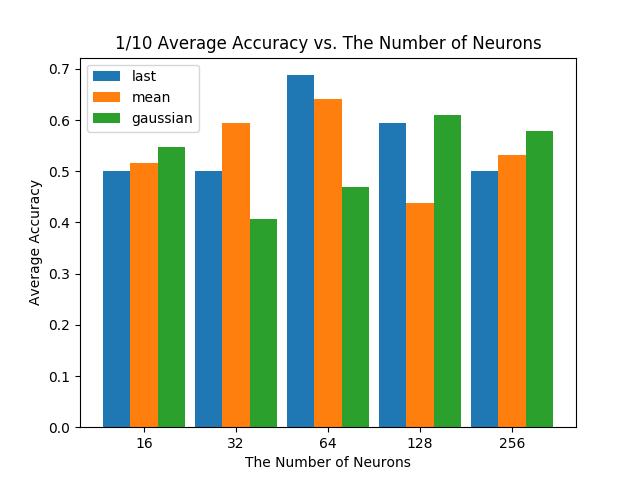
\includegraphics[width=0.75\textwidth]{pictures/result_pictures/filtered_1_10_result.png}
    \caption{Result of 1 over 10 from {\em filtered dataset}}
    \label{fig:filter_1_10}
\end{figure}

\begin{table}[!t]
\centering
\caption{{\em last} method on 1 over 10 Re-sampled {\em filtered dataset}}
\label{tbl:last_1_10}
\begin{tabular}{|c|c|c|c|c|c|c|}
\hline
\multirow{2}{*}{Test} & \multirow{2}{*}{CV} & \multicolumn{5}{c|}{The number of neurans}                               \\ \cline{3-7}
                      &                     & 16           & 32           & 64           & 128          & 256          \\ \hline
\multirow{4}{*}{1}    & 1                   & 0.5          & 0.25         & 1            & 0.5          & 0.5          \\ \cline{2-7}
                      & 2                   & 0.75         & 0.75         & 0.5          & 0.5          & 0.5          \\ \cline{2-7}
                      & 3                   & 1            & 0.5          & 0.5          & 0.75         & 0.5          \\ \cline{2-7}
                      & 4                   & 0.5          & 0.5          & 0.75         & 0.5          & 0.5          \\ \hline
\multirow{4}{*}{2}    & 1                   & 0.5          & 0.75         & 0.75         & 0.75         & 0.75         \\ \cline{2-7}
                      & 2                   & 0.25         & 0.25         & 0.75         & 0.5          & 0.25         \\ \cline{2-7}
                      & 3                   & 0.5          & 0.5          & 0.25         & 0.75         & 0.25         \\ \cline{2-7}
                      & 4                   & 0.25         & 0.25         & 0.5          & 0.25         & 0.75         \\ \hline
\multirow{4}{*}{3}    & 1                   & 0.75         & 0.25         & 1            & 0.75         & 0.25         \\ \cline{2-7}
                      & 2                   & 0.25         & 0.5          & 0.75         & 0.5          & 1            \\ \cline{2-7}
                      & 3                   & 0.5          & 0.75         & 0.75         & 0.5          & 0.5          \\ \cline{2-7}
                      & 4                   & 0.5          & 0.25         & 0.75         & 0.75         & 0.5          \\ \hline
\multirow{4}{*}{4}    & 1                   & 0.75         & 0.5          & 0.5          & 0.5          & 0.5          \\ \cline{2-7}
                      & 2                   & 0.25         & 0.5          & 0.5          & 1            & 0.25         \\ \cline{2-7}
                      & 3                   & 0            & 0.75         & 1            & 0.75         & 0.25         \\ \cline{2-7}
                      & 4                   & 0.75         & 0.75         & 0.75         & 0.25         & 0.75         \\ \hline
\multicolumn{2}{|c|}{Mean}                  & 0.5          & 0.5          & 0.6875       & 0.59375      & 0.5          \\ \hline
\multicolumn{2}{|c|}{Std}                   & 0.2581988897 & 0.2041241452 & 0.2140872096 & 0.2015564437 & 0.2236067977 \\ \hline
\end{tabular}
\end{table}

\begin{table}[!t]
\centering
\caption{{\em mean} method on 1 over 10 Re-sampled {\em filtered dataset}}
\label{tbl:mean_1_10}
\begin{tabular}{|c|c|c|c|c|c|c|}
\hline
\multirow{2}{*}{Test} & \multirow{2}{*}{CV} & \multicolumn{5}{c|}{The number of neurans}                               \\ \cline{3-7}
                      &                     & 16           & 32           & 64           & 128          & 256          \\ \hline
\multirow{4}{*}{1}    & 1                   & 0.75         & 0.75         & 0.75         & 0.25         & 0.75         \\ \cline{2-7}
                      & 2                   & 0.25         & 0.5          & 0.75         & 0.25         & 0.25         \\ \cline{2-7}
                      & 3                   & 0.75         & 0.75         & 0.75         & 0.5          & 0.5          \\ \cline{2-7}
                      & 4                   & 0.75         & 0.75         & 0.75         & 0            & 0.25         \\ \hline
\multirow{4}{*}{2}    & 1                   & 0.5          & 0.5          & 0.75         & 0.25         & 0.5          \\ \cline{2-7}
                      & 2                   & 0.5          & 0.25         & 0.75         & 0.5          & 0.5          \\ \cline{2-7}
                      & 3                   & 0.25         & 0.25         & 0.5          & 0.75         & 0.75         \\ \cline{2-7}
                      & 4                   & 0.5          & 0.75         & 0.25         & 0.5          & 0.5          \\ \hline
\multirow{4}{*}{3}    & 1                   & 0.5          & 0.5          & 0.75         & 0.5          & 0.5          \\ \cline{2-7}
                      & 2                   & 0.75         & 0.75         & 0.25         & 0.5          & 0.75         \\ \cline{2-7}
                      & 3                   & 0.5          & 0.5          & 1            & 0.5          & 0.5          \\ \cline{2-7}
                      & 4                   & 0.75         & 0.75         & 0.5          & 0.25         & 0.5          \\ \hline
\multirow{4}{*}{4}    & 1                   & 0.5          & 0.5          & 0.5          & 0.75         & 0.5          \\ \cline{2-7}
                      & 2                   & 0.25         & 0.5          & 0.5          & 0.25         & 0.75         \\ \cline{2-7}
                      & 3                   & 0.5          & 1            & 0.5          & 0.5          & 0.5          \\ \cline{2-7}
                      & 4                   & 0.25         & 0.5          & 1            & 0.75         & 0.5          \\ \hline
\multicolumn{2}{|c|}{Mean}                  & 0.515625     & 0.59375      & 0.640625     & 0.4375       & 0.53125      \\ \hline
\multicolumn{2}{|c|}{Std}                   & 0.1929756029 & 0.2015564437 & 0.2230237282 & 0.2140872096 & 0.1547847968 \\ \hline
\end{tabular}
\end{table}

\begin{table}[!t]
\centering
\caption{{\em gaussian} method on 1 over 10 Re-sampled {\em filtered dataset}}
\label{tbl:gaussian_1_10}
\begin{tabular}{|c|c|c|c|c|c|c|}
\hline
\multirow{2}{*}{Test} & \multirow{2}{*}{CV} & \multicolumn{5}{c|}{The number of neurans}                               \\ \cline{3-7}
                      &                     & 16           & 32           & 64           & 128          & 256          \\ \hline
\multirow{4}{*}{1}    & 1                   & 0.5          & 0.5          & 0.75         & 0.5          & 0.75         \\ \cline{2-7}
                      & 2                   & 0.5          & 0.75         & 0.5          & 0.5          & 0.5          \\ \cline{2-7}
                      & 3                   & 0.25         & 0.5          & 0.5          & 0.75         & 0.5          \\ \cline{2-7}
                      & 4                   & 0.5          & 0.5          & 0.5          & 0.5          & 0.75         \\ \hline
\multirow{4}{*}{2}    & 1                   & 1            & 0.5          & 0.25         & 0.5          & 0            \\ \cline{2-7}
                      & 2                   & 0.75         & 0.25         & 0.75         & 0.25         & 1            \\ \cline{2-7}
                      & 3                   & 0.5          & 0            & 0.75         & 0.5          & 0.5          \\ \cline{2-7}
                      & 4                   & 0.25         & 0.25         & 0.25         & 0.75         & 0.75         \\ \hline
\multirow{4}{*}{3}    & 1                   & 0.75         & 0.25         & 0.5          & 1            & 0.5          \\ \cline{2-7}
                      & 2                   & 0.5          & 0.5          & 0            & 1            & 0.5          \\ \cline{2-7}
                      & 3                   & 0.75         & 0.5          & 0.5          & 0.5          & 0.75         \\ \cline{2-7}
                      & 4                   & 0.25         & 0.5          & 0.5          & 0.75         & 0.5          \\ \hline
\multirow{4}{*}{4}    & 1                   & 0.5          & 0.25         & 0.5          & 0.75         & 0.5          \\ \cline{2-7}
                      & 2                   & 0.75         & 0.5          & 0.75         & 0.75         & 0.75         \\ \cline{2-7}
                      & 3                   & 0.5          & 0.5          & 0.5          & 0            & 0.25         \\ \cline{2-7}
                      & 4                   & 0.5          & 0.25         & 0            & 0.75         & 0.75         \\ \hline
\multicolumn{2}{|c|}{Mean}                  & 0.546875     & 0.40625      & 0.46875      & 0.609375     & 0.578125     \\ \hline
\multicolumn{2}{|c|}{Std}                   & 0.2085415626 & 0.1796988221 & 0.2393567769 & 0.2576941016 & 0.2366211811 \\ \hline
\end{tabular}
\end{table}

\begin{table}[!t]
\centering
\caption{{\em last} Test Time with 1 over 10 Re-sampled {\em filtered dataset}}
\label{tbl:last_1_10_time}
\begin{tabular}{|c|c|c|c|c|c|}
\hline
\multirow{2}{*}{Test}      & \multicolumn{5}{c|}{The number of neurans}                                                                                                               \\ \cline{2-6}
                           & 16                           & 32                           & 64                           & 128                          & 256                          \\ \hline
1                          & 2:13:13                      & 2:21:07                      & 3:02:52                      & 4:25:58                      & 6:42:39                      \\ \hline
2                          & 2:12:00                      & 2:19:41                      & 3:09:02                      & 4:35:59                      & 6:55:31                      \\ \hline
3                          & 2:14:25                      & 2:22:30                      & 3:03:53                      & 4:27:02                      & 6:50:01                      \\ \hline
4                          & 2:08:12                      & 2:21:27                      & 3:02:30                      & 4:24:37                      & 5:55:15                      \\ \hline
\multicolumn{1}{|l|}{Mean} & \multicolumn{1}{l|}{2:11:58} & \multicolumn{1}{l|}{2:21:11} & \multicolumn{1}{l|}{3:04:34} & \multicolumn{1}{l|}{4:28:24} & \multicolumn{1}{l|}{6:35:52} \\ \hline
\end{tabular}
\end{table}

\begin{table}[!t]
\centering
\caption{{\em mean} Test Time with 1 over 10 Re-sampled {\em filtered dataset}}
\label{tbl:mean_1_10_time}
\begin{tabular}{|c|c|c|c|c|c|}
\hline
\multirow{2}{*}{Test}      & \multicolumn{5}{c|}{The number of neurans}                                                                                                               \\ \cline{2-6}
                           & 16                           & 32                           & 64                           & 128                          & 256                          \\ \hline
1                          & 1:50:32                      & 2:26:14                      & 2:42:42                      & 4:23:05                      & 6:50:48                      \\ \hline
2                          & 1:59:38                      & 3:02:34                      & 3:20:51                      & 4:28:45                      & 7:10:39                      \\ \hline
3                          & 1:57:17                      & 1:52:17                      & 2:49:14                      & 4:16:30                      & 6:48:25                      \\ \hline
4                          & 2:09:51                      & 2:16:48                      & 3:28:13                      & 4:36:27                      & 7:02:04                      \\ \hline
\multicolumn{1}{|l|}{Mean} & \multicolumn{1}{l|}{1:59:20} & \multicolumn{1}{l|}{2:24:28} & \multicolumn{1}{l|}{3:05:15} & \multicolumn{1}{l|}{4:26:12} & \multicolumn{1}{l|}{6:57:59} \\ \hline
\end{tabular}
\end{table}

\begin{table}[!t]
\centering
\caption{{\em gaussian} Test Time with 1 over 10 Re-sampled {\em filtered dataset}}
\label{tbl:gaussian_1_10_time}
\begin{tabular}{|c|c|c|c|c|c|}
\hline
\multirow{2}{*}{Test}      & \multicolumn{5}{c|}{The number of neurans}                                                                                                               \\ \cline{2-6}
                           & 16                           & 32                           & 64                           & 128                          & 256                          \\ \hline
1                          & 2:03:47                      & 2:36:34                      & 2:52:38                      & 4:18:07                      & 6:50:52                      \\ \hline
2                          & 1:50:33                      & 2:27:43                      & 3:26:58                      & 4:39:46                      & 7:07:22                      \\ \hline
3                          & 2:10:52                      & 2:03:13                      & 2:39:12                      & 4:34:03                      & 6:42:58                      \\ \hline
4                          & 1:56:08                      & 2:21:53                      & 3:25:02                      & 4:24:05                      & 6:47:56                      \\ \hline
\multicolumn{1}{|l|}{Mean} & \multicolumn{1}{l|}{2:00:20} & \multicolumn{1}{l|}{2:22:21} & \multicolumn{1}{l|}{3:05:58} & \multicolumn{1}{l|}{4:29:00} & \multicolumn{1}{l|}{6:52:17} \\ \hline
\end{tabular}
\end{table}


\section{Experiments with {\em raw dataset}}
The second part of experiments used {\em raw dataset} which has 98 features. The dataset was re-sampled only by 1 over 10 with {\em last} method. This is because the test time with {\em second model} with SAE and {\em third model} with MAE took much more than the test time with {\em first model} and from the result of the first part of experiments, the best overall performance was from 1 over 10 re-sampled data and the best performance was from {\em last} method.

\subsection{Comparison of results from three models}
\begin{figure}[t!]
    \centering
    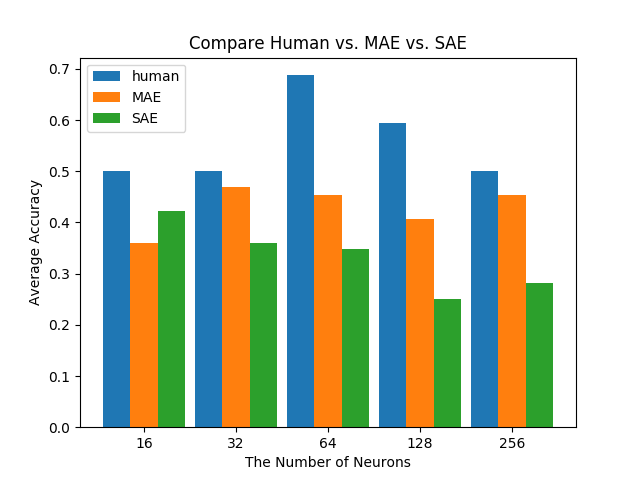
\includegraphics[width=0.75\textwidth]{pictures/result_pictures/compare_result_last_1_10.png}
    \caption{Result of three models with {\em last} method}
    \label{fig:compare_result_last_1_10}
\end{figure}

Figure \ref{fig:compare_result_last_1_10} compares the performance from the reduced dimensions data by human, MAE, and SAE. Table \ref{tbl:mae_last_1_10} and Table \ref{tbl:sae_last_1_10} show the detailed result of MAE and SAE respectively and Table \ref{tbl:mae_last_1_10_time} and Table \ref{tbl:sae_last_1_10_time} shows the test time for MAE and SAE respectively.

The overall average accuracy from SAE is 0.3375 (33.75\%) and the overall average accuracy from MAE is 0.428125 (42.8125\%). Both performance are much lower than 0.540625 (54.0625\%) performance from the experiments with data filtered by human. Next subsection explains the reasons why SAE and MAE gave worse performance.

\begin{table}[!t]
\centering
\caption{MAE, {\em last} method on 1 over 10 Re-sampled {\em raw dataset}}
\label{tbl:mae_last_1_10}
\begin{tabular}{|c|c|c|c|c|c|c|}
\hline
\multirow{2}{*}{Test} & \multirow{2}{*}{CV} & \multicolumn{5}{c|}{The number of neurans}                               \\ \cline{3-7}
                      &                     & 16           & 32           & 64           & 128          & 256          \\ \hline
\multirow{4}{*}{1}    & 1                   & 0.25         & 0.75         & 0.25         & 0            & 0.5          \\ \cline{2-7}
                      & 2                   & 0.5          & 0.5          & 0.5          & 0.5          & 0.5          \\ \cline{2-7}
                      & 3                   & 0.5          & 0.5          & 0.5          & 0.5          & 0.5          \\ \cline{2-7}
                      & 4                   & 0.25         & 0.25         & 0.5          & 0.5          & 0.5          \\ \hline
\multirow{4}{*}{2}    & 1                   & 0.75         & 0.75         & 0.5          & 0.75         & 0.5          \\ \cline{2-7}
                      & 2                   & 0.5          & 1            & 0.5          & 0.5          & 0.5          \\ \cline{2-7}
                      & 3                   & 0.25         & 0.25         & 0.75         & 0.5          & 0.5          \\ \cline{2-7}
                      & 4                   & 0.25         & 0.75         & 0.25         & 0.25         & 0.5          \\ \hline
\multirow{4}{*}{3}    & 1                   & 0            & 0.25         & 0.75         & 0            & 0.5          \\ \cline{2-7}
                      & 2                   & 0.25         & 0.5          & 0.25         & 0.5          & 0.25         \\ \cline{2-7}
                      & 3                   & 0.25         & 0.25         & 0.75         & 0.5          & 0.25         \\ \cline{2-7}
                      & 4                   & 1            & 0.5          & 0.5          & 0.5          & 0.5          \\ \hline
\multirow{4}{*}{4}    & 1                   & 0.5          & 0.5          & 0.25         & 0.5          & 0.75         \\ \cline{2-7}
                      & 2                   & 0            & 0.5          & 0.5          & 0.25         & 0.25         \\ \cline{2-7}
                      & 3                   & 0            & 0.25         & 0            & 0.25         & 0.5          \\ \cline{2-7}
                      & 4                   & 0.5          & 0            & 0.5          & 0.5          & 0.25         \\ \hline
\multicolumn{2}{|c|}{Mean}                  & 0.359375     & 0.46875      & 0.453125     & 0.40625      & 0.453125     \\ \hline
\multicolumn{2}{|c|}{Std}                   & 0.2733854117 & 0.2561737691 & 0.2085415626 & 0.2015564437 & 0.1359764073 \\ \hline
\end{tabular}
\end{table}

\begin{table}[!t]
\centering
\caption{MAE, {\em last} Test Time with 1 over 10 Re-sampled {\em raw dataset}}
\label{tbl:mae_last_1_10_time}
\begin{tabular}{|c|c|c|c|c|c|}
\hline
\multirow{2}{*}{Test} & \multicolumn{5}{c|}{The number of neurans}       \\ \cline{2-6}
                      & 16      & 32      & 64      & 128     & 256      \\ \hline
1                     & 6:59:30 & 6:59:33 & 8:13:06 & 9:21:31 & 11:40:13 \\ \hline
2                     & 6:25:43 & 6:58:03 & 7:50:26 & 8:52:23 & 11:06:24 \\ \hline
3                     & 6:14:18 & 6:43:07 & 7:12:21 & 8:17:23 & 10:17:59 \\ \hline
4                     & 7:07:35 & 4:52:05 & 5:28:28 & 6:38:07 & 8:43:28  \\ \hline
Mean                  & 6:41:47 & 6:23:12 & 7:11:05 & 8:17:21 & 10:27:01 \\ \hline
\end{tabular}
\end{table}

\begin{table}[!t]
\centering
\caption{SAE, {\em last} method on 1 over 10 Re-sampled {\em raw dataset}}
\label{tbl:sae_last_1_10}
\begin{tabular}{|c|c|c|c|c|c|c|}
\hline
\multirow{2}{*}{Test} & \multirow{2}{*}{CV} & \multicolumn{5}{c|}{The number of neurans}                               \\ \cline{3-7}
                      &                     & 16           & 32           & 64           & 128          & 256          \\ \hline
\multirow{4}{*}{1}    & 1                   & 0.75         & 0.75         & 0.5          & 0            & 0.5          \\ \cline{2-7}
                      & 2                   & 0.25         & 0            & 0.5          & 0.25         & 0.25         \\ \cline{2-7}
                      & 3                   & 0.75         & 0            & 0            & 0.25         & 0.5          \\ \cline{2-7}
                      & 4                   & 0.5          & 0.5          & 0.5          & 0.5          & 0.75         \\ \hline
\multirow{4}{*}{2}    & 1                   & 0.5          & 0.5          & 0.25         & 0.75         & 0.5          \\ \cline{2-7}
                      & 2                   & 0.5          & 0.25         & 0            & 0            & 0            \\ \cline{2-7}
                      & 3                   & 0.5          & 0            & 0.25         & 0.5          & 0.75         \\ \cline{2-7}
                      & 4                   & 0.25         & 0.75         & 0.5          & 0.5          & 0            \\ \hline
\multirow{4}{*}{3}    & 1                   & 0.25         & 0.25         & 0.5          & 0.25         & 0            \\ \cline{2-7}
                      & 2                   & 0.25         & 0.25         & 0.5          & 0.25         & 0.5          \\ \cline{2-7}
                      & 3                   & 0.25         & 0.25         & 0.25         & 0.25         & 0.25         \\ \cline{2-7}
                      & 4                   & 0.75         & 0.5          & 0.25         & 0            & 0            \\ \hline
\multirow{4}{*}{4}    & 1                   & 0.5          & 0.25         & 0.25         & 0.25         & 0.25         \\ \cline{2-7}
                      & 2                   & 0.25         & 0.75         & 0            & 0.5          & 0            \\ \cline{2-7}
                      & 3                   & 0.25         & 0.25         & 0.5          & 0            & 0            \\ \cline{2-7}
                      & 4                   & 0.25         & 0.5          & 0.75         & 0.25         & 0.25         \\ \hline
\multicolumn{2}{|c|}{Mean}                  & 0.421875     & 0.359375     & 0.34375      & 0.28125      & 0.28125      \\ \hline
\multicolumn{2}{|c|}{Std}                   & 0.1983000672 & 0.2576941016 & 0.2212653008 & 0.2212653008 & 0.2719528145 \\ \hline
\end{tabular}
\end{table}

\begin{table}[!t]
\centering
\caption{SAE, {\em last} Test Time with 1 over 10 Re-sampled {\em raw dataset}}
\label{tbl:sae_last_1_10_time}
\begin{tabular}{|c|c|c|c|c|c|}
\hline
\multirow{2}{*}{Test} & \multicolumn{5}{c|}{The number of neurans}      \\ \cline{2-6}
                      & 16      & 32      & 64      & 128     & 256     \\ \hline
1                     & 4:20:50 & 4:58:12 & 7:44:27 & 6:42:45 & 8:38:18 \\ \hline
2                     & 3:48:20 & 3:51:03 & 5:16:07 & 6:02:29 & 8:24:17 \\ \hline
3                     & 3:50:54 & 4:47:55 & 5:03:59 & 6:29:31 & 8:48:47 \\ \hline
4                     & 3:40:38 & 4:09:14 & 4:56:10 & 6:09:21 & 8:24:11 \\ \hline
Mean                  & 3:55:11 & 4:26:36 & 5:45:11 & 6:21:02 & 8:33:53 \\ \hline
\end{tabular}
\end{table}


\subsection{Analysis Training LSTM in {\em second model} and {\em third model}}
The difference between {\em first model} and other models is that other models have AE. Therefore, AE layer from {\em second model} and {\em third model} caused worse performance. The first evidence of this can be found during training LSTM in both models. Figure \ref{fig:sae_accuracy} and Figure \ref{fig:mae_accuracy} show the accuracy of the result from LSTM on each iterations during training. Figure \ref{fig:sae_loss} and Figure \ref{fig:mae_loss} show the loss (error) on each iterations during training. Table \ref{tbl:sae_16_accuracy}, Table \ref{tbl:sae_32_accuracy}, Table \ref{tbl:sae_64_accuracy}, Table \ref{tbl:sae_128_accuracy}, and Table \ref{tbl:sae_256_accuracy} show the details of the train accuracy from {\em second model} with 16 neurons, 32 neurons, 64 neurons, 128 neurons, and 256 neurons. Table \ref{tbl:sae_16_loss}, Table \ref{tbl:sae_32_loss}, Table \ref{tbl:sae_64_loss}, Table \ref{tbl:sae_128_loss}, and Table \ref{tbl:sae_256_loss} show the details of the train loss from {\em second model} with 16 neurons, 32 neurons, 64 neurons, 128 neurons, and 256 neurons. Table \ref{tbl:mae_16_accuracy}, Table \ref{tbl:mae_32_accuracy}, Table \ref{tbl:mae_64_accuracy}, Table \ref{tbl:mae_128_accuracy}, and Table \ref{tbl:mae_256_accuracy} show the details of the train accuracy from {\em third model} with 16 neurons, 32 neurons, 64 neurons, 128 neurons, and 256 neurons. Table \ref{tbl:mae_16_loss}, Table \ref{tbl:mae_32_loss}, Table \ref{tbl:mae_64_loss}, Table \ref{tbl:mae_128_loss}, and Table \ref{tbl:mae_256_loss} show the details of the train loss from {\em third model} with 16 neurons, 32 neurons, 64 neurons, 128 neurons, and 256 neurons.

Training LSTM in {\em second model} and {\em third model} were slow and most cases did not reach accuracy 1 (100\%) while the training LSTM in {\em first model} easily reached accuracy 1 (100\%). It implies that the data fed to LSTM had noise or problems. It also means that AE in {\em second model} and {\em third model} did not work correctly. The next subsection covers more detailed explanation about the error from AE in {\em second model} and {\em third model}.

\begin{figure}[t!]
    \centering
    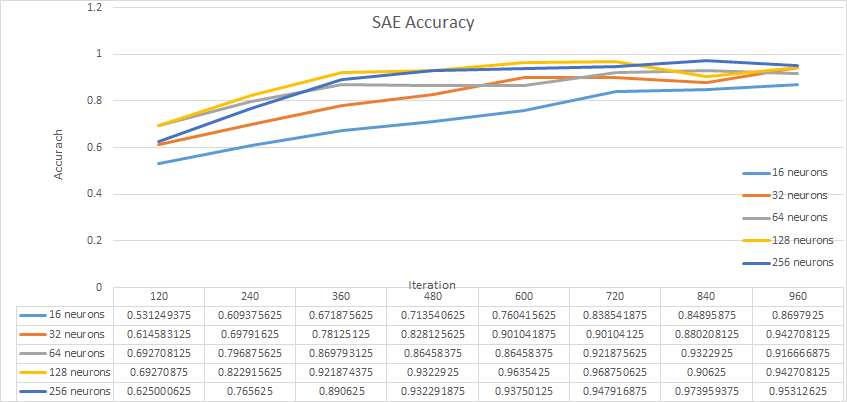
\includegraphics[width=\textwidth]{pictures/result_pictures/SAE_Accuracy.png}
    \caption{SAE Training Accuracy}
    \label{fig:sae_accuracy}
\end{figure}

\begin{figure}[t!]
    \centering
    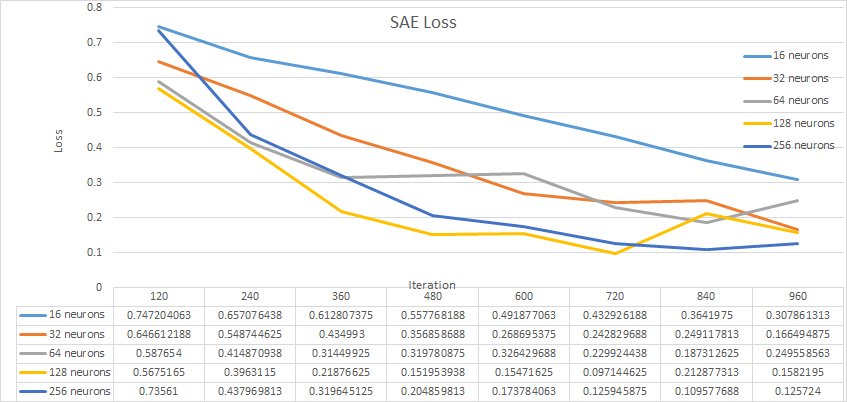
\includegraphics[width=\textwidth]{pictures/result_pictures/SAE_Loss.png}
    \caption{SAE Training Loss}
    \label{fig:sae_loss}
\end{figure}

\begin{table}[!t]
\centering
\caption{SAE, 16 Neuron Training Accuracy}
\label{tbl:sae_16_accuracy}
\resizebox{\textwidth}{!}{\begin{tabular}{|c|c|c|c|c|c|c|c|c|c|c|}
\hline
\multirow{2}{*}{Test} & \multirow{2}{*}{CV} & \multicolumn{9}{c|}{Iterations}                                                                                                                                                \\ \cline{3-11} 
                      &                     & 0             & 120         & 240           & 360          & 480          & 600                              & 720                               & 840          & 960          \\ \hline
\multirow{4}{*}{1}    & 1                   & 0.58333       & 0.66667     & 0.66667       & 0.75         & 0.75         & 0.83333                          & 1                                 & 0.91667      & 0.91667      \\ \cline{2-11} 
                      & 2                   & 0.5           & 0.5         & 0.66667       & 0.83333      & 0.83333      & 0.91667                          & 1                                 & 1            & 1            \\ \cline{2-11} 
                      & 3                   & 0.41667       & 0.58333     & 0.66667       & 0.91667      & 0.83333      & 0.83333                          & 0.91667                           & 1            & 0.91667      \\ \cline{2-11} 
                      & 4                   & 0.5           & 0.58333     & 0.58333       & 0.58333      & 0.58333      & 0.75                             & 0.91667                           & 0.91667      & 0.91667      \\ \hline
\multirow{4}{*}{2}    & 1                   & 0.5           & 0.58333     & 0.5           & 0.5          & 0.5          & 0.58333                          & 0.75                              & 0.75         & 0.83333      \\ \cline{2-11} 
                      & 2                   & 0.5           & 0.58333     & 0.75          & 0.75         & 0.83333      & 0.91667                          & 1                                 & 1            & 1            \\ \cline{2-11} 
                      & 3                   & 0.5           & 0.66667     & 0.75          & 0.75         & 0.83333      & 0.91667                          & 0.83333                           & 0.83333      & 0.91667      \\ \cline{2-11} 
                      & 4                   & 0.5           & 0.5         & 0.5           & 0.5          & 0.58333      & 0.5                              & 0.58333                           & 0.66667      & 0.66667      \\ \hline
\multirow{4}{*}{3}    & 1                   & 0.5           & 0.5         & 0.58333       & 0.58333      & 0.75         & 0.58333                          & 0.58333                           & 0.75         & 0.83333      \\ \cline{2-11} 
                      & 2                   & 0.5           & 0.41667     & 0.5           & 0.66667      & 0.66667      & 0.75                             & 0.75                              & 0.75         & 0.91667      \\ \cline{2-11} 
                      & 3                   & 0.5           & 0.33333     & 0.5           & 0.41667      & 0.5          & 0.58333                          & 0.91667                           & 0.75         & 0.75         \\ \cline{2-11} 
                      & 4                   & 0.33333       & 0.66667     & 0.66667       & 0.66667      & 0.83333      & 0.83333                          & 0.91667                           & 1            & 1            \\ \hline
\multirow{4}{*}{4}    & 1                   & 0.5           & 0.58333     & 0.58333       & 0.66667      & 0.75         & 0.83333                          & 0.83333                           & 0.83333      & 0.75         \\ \cline{2-11} 
                      & 2                   & 0.5           & 0.33333     & 0.66667       & 0.83333      & 0.66667      & 0.75                             & 0.75                              & 0.66667      & 0.83333      \\ \cline{2-11} 
                      & 3                   & 0.41667       & 0.58333     & 0.66667       & 0.66667      & 0.75         & 0.83333                          & 0.91667                           & 0.91667      & 0.91667      \\ \cline{2-11} 
                      & 4                   & 0.5           & 0.41667     & 0.5           & 0.66667      & 0.75         & 0.75                             & 0.75                              & 0.83333      & 0.75         \\ \hline
\multicolumn{2}{|c|}{Mean}                  & 0.484375      & 0.531249375 & 0.609375625   & 0.671875625  & 0.713540625  & 0.760415625                      & 0.838541875                       & 0.84895875   & 0.8697925    \\ \hline
\multicolumn{2}{|c|}{Std}                   & 0.05459200528 & 0.109185219 & 0.08985045449 & 0.1342629486 & 0.1177274886 & \multicolumn{1}{l|}{0.132201113} & \multicolumn{1}{l|}{0.1342647589} & 0.1187071365 & 0.1007786353 \\ \hline
\end{tabular}}
\end{table}

\begin{table}[!t]
\centering
\caption{SAE, 32 Neuron Training Accuracy}
\label{tbl:sae_32_accuracy}
\resizebox{\textwidth}{!}{\begin{tabular}{|c|c|c|c|c|c|c|c|c|c|c|}
\hline
\multirow{2}{*}{Test} & \multirow{2}{*}{CV} & \multicolumn{9}{c|}{Iterations}                                                                                                                                                 \\ \cline{3-11} 
                      &                     & 0             & 120          & 240          & 360          & 480          & 600                              & 720                               & 840          & 960           \\ \hline
\multirow{4}{*}{1}    & 1                   & 0.41667       & 0.66667      & 0.91667      & 0.91667      & 0.83333      & 0.91667                          & 1                                 & 0.91667      & 1             \\ \cline{2-11} 
                      & 2                   & 0.5           & 0.75         & 0.66667      & 0.75         & 0.83333      & 1                                & 1                                 & 1            & 1             \\ \cline{2-11} 
                      & 3                   & 0.5           & 0.75         & 0.66667      & 0.75         & 0.91667      & 1                                & 0.91667                           & 0.58333      & 0.75          \\ \cline{2-11} 
                      & 4                   & 0.5           & 0.58333      & 0.66667      & 0.66667      & 0.91667      & 0.91667                          & 1                                 & 1            & 1             \\ \hline
\multirow{4}{*}{2}    & 1                   & 0.5           & 0.75         & 0.83333      & 0.83333      & 0.91667      & 1                                & 0.91667                           & 0.91667      & 1             \\ \cline{2-11} 
                      & 2                   & 0.41667       & 0.58333      & 0.83333      & 0.91667      & 1            & 0.91667                          & 1                                 & 0.91667      & 1             \\ \cline{2-11} 
                      & 3                   & 0.5           & 0.66667      & 0.58333      & 0.66667      & 0.66667      & 0.66667                          & 0.75                              & 0.75         & 0.83333       \\ \cline{2-11} 
                      & 4                   & 0.5           & 0.33333      & 0.41667      & 0.5          & 0.5          & 0.83333                          & 0.58333                           & 0.83333      & 0.83333       \\ \hline
\multirow{4}{*}{3}    & 1                   & 0.33333       & 0.75         & 0.83333      & 0.91667      & 0.91667      & 1                                & 1                                 & 1            & 1             \\ \cline{2-11} 
                      & 2                   & 0.5           & 0.66667      & 0.75         & 0.91667      & 0.83333      & 1                                & 0.83333                           & 1            & 1             \\ \cline{2-11} 
                      & 3                   & 0.58333       & 0.66667      & 0.83333      & 0.91667      & 1            & 0.83333                          & 0.91667                           & 0.83333      & 1             \\ \cline{2-11} 
                      & 4                   & 0.5           & 0.5          & 0.58333      & 0.66667      & 0.83333      & 0.91667                          & 1                                 & 0.75         & 1             \\ \hline
\multirow{4}{*}{4}    & 1                   & 0.5           & 0.5          & 0.5          & 0.83333      & 0.66667      & 0.83333                          & 0.83333                           & 0.83333      & 0.83333       \\ \cline{2-11} 
                      & 2                   & 0.5           & 0.58333      & 0.75         & 0.75         & 0.75         & 0.75                             & 0.83333                           & 0.83333      & 0.91667       \\ \cline{2-11} 
                      & 3                   & 0.5           & 0.5          & 0.58333      & 0.58333      & 0.75         & 0.83333                          & 0.83333                           & 0.91667      & 0.91667       \\ \cline{2-11} 
                      & 4                   & 0.33333       & 0.58333      & 0.75         & 0.91667      & 0.91667      & 1                                & 1                                 & 1            & 1             \\ \hline
\multicolumn{2}{|c|}{Mean}                  & 0.473958125   & 0.614583125  & 0.69791625   & 0.78125125   & 0.828125625  & 0.901041875                      & 0.90104125                        & 0.880208125  & 0.942708125   \\ \hline
\multicolumn{2}{|c|}{Std}                   & 0.06610021505 & 0.1173602203 & 0.1390271423 & 0.1356577598 & 0.1342634141 & \multicolumn{1}{l|}{0.101920437} & \multicolumn{1}{l|}{0.1187085405} & 0.1177294942 & 0.08454060225 \\ \hline
\end{tabular}}
\end{table}

\begin{table}[!t]
\centering
\caption{SAE, 64 Neuron Training Accuracy}
\label{tbl:sae_64_accuracy}
\resizebox{\textwidth}{!}{\begin{tabular}{|c|c|c|c|c|c|c|c|c|c|c|}
\hline
\multirow{2}{*}{Test} & \multirow{2}{*}{CV} & \multicolumn{9}{c|}{Iterations}                                                                                                                                               \\ \cline{3-11} 
                      &                     & 0             & 120         & 240         & 360          & 480        & 600                               & 720                                & 840           & 960          \\ \hline
\multirow{4}{*}{1}    & 1                   & 0.5           & 0.58333     & 0.66667     & 0.66667      & 0.75       & 0.83333                           & 1                                  & 1             & 0.66667      \\ \cline{2-11} 
                      & 2                   & 0.66667       & 0.66667     & 0.83333     & 0.91667      & 0.91667    & 0.41667                           & 0.75                               & 0.66667       & 0.5          \\ \cline{2-11} 
                      & 3                   & 0.5           & 0.5         & 0.66667     & 0.91667      & 1          & 1                                 & 1                                  & 1             & 1            \\ \cline{2-11} 
                      & 4                   & 0.5           & 0.75        & 0.66667     & 0.83333      & 0.91667    & 0.91667                           & 0.91667                            & 1             & 1            \\ \hline
\multirow{4}{*}{2}    & 1                   & 0.58333       & 0.83333     & 0.83333     & 0.66667      & 0.66667    & 0.66667                           & 0.83333                            & 0.83333       & 0.83333      \\ \cline{2-11} 
                      & 2                   & 0.5           & 0.5         & 0.75        & 0.91667      & 0.58333    & 0.83333                           & 1                                  & 1             & 1            \\ \cline{2-11} 
                      & 3                   & 0.5           & 0.58333     & 0.91667     & 1            & 1          & 1                                 & 1                                  & 1             & 1            \\ \cline{2-11} 
                      & 4                   & 0.5           & 0.66667     & 0.91667     & 0.83333      & 0.91667    & 1                                 & 0.91667                            & 0.91667       & 0.91667      \\ \hline
\multirow{4}{*}{3}    & 1                   & 0.58333       & 0.83333     & 0.91667     & 1            & 1          & 1                                 & 1                                  & 1             & 1            \\ \cline{2-11} 
                      & 2                   & 0.5           & 0.58333     & 0.5         & 0.66667      & 0.75       & 0.83333                           & 0.75                               & 0.91667       & 0.83333      \\ \cline{2-11} 
                      & 3                   & 0.58333       & 0.75        & 0.91667     & 0.91667      & 1          & 0.91667                           & 1                                  & 1             & 1            \\ \cline{2-11} 
                      & 4                   & 0.5           & 0.66667     & 0.75        & 0.83333      & 0.91667    & 0.91667                           & 0.91667                            & 0.91667       & 1            \\ \hline
\multirow{4}{*}{4}    & 1                   & 0.58333       & 0.66667     & 0.83333     & 0.91667      & 1          & 0.91667                           & 0.91667                            & 0.91667       & 1            \\ \cline{2-11} 
                      & 2                   & 0.41667       & 0.75        & 0.83333     & 0.91667      & 0.83333    & 0.83333                           & 0.91667                            & 0.91667       & 0.91667      \\ \cline{2-11} 
                      & 3                   & 0.5           & 0.91667     & 0.83333     & 0.91667      & 1          & 1                                 & 1                                  & 1             & 1            \\ \cline{2-11} 
                      & 4                   & 0.41667       & 0.83333     & 0.91667     & 1            & 0.58333    & 0.75                              & 0.83333                            & 0.83333       & 1            \\ \hline
\multicolumn{2}{|c|}{Mean}                  & 0.520833125   & 0.692708125 & 0.796875625 & 0.869793125  & 0.86458375 & 0.86458375                        & 0.921875625                        & 0.9322925     & 0.916666875  \\ \hline
\multicolumn{2}{|c|}{Std}                   & 0.06454864664 & 0.124419997 & 0.12159725  & 0.1137275314 & 0.1517652  & \multicolumn{1}{l|}{0.1547843482} & \multicolumn{1}{l|}{0.08855225756} & 0.09238947353 & 0.1459323791 \\ \hline
\end{tabular}}
\end{table}

\begin{table}[!t]
\centering
\caption{SAE, 128 Neuron Training Accuracy}
\label{tbl:sae_128_accuracy}
\resizebox{\textwidth}{!}{\begin{tabular}{|c|c|c|c|c|c|c|c|c|c|c|}
\hline
\multirow{2}{*}{Test} & \multirow{2}{*}{CV} & \multicolumn{9}{c|}{Iterations}                                                                                                                                                      \\ \cline{3-11} 
                      &                     & 0             & 120           & 240           & 360         & 480           & 600                                & 720                                & 840          & 960           \\ \hline
\multirow{4}{*}{1}    & 1                   & 0.5           & 0.66667       & 0.91667       & 1           & 1             & 1                                  & 1                                  & 1            & 1             \\ \cline{2-11} 
                      & 2                   & 0.58333       & 0.75          & 0.83333       & 1           & 0.91667       & 1                                  & 1                                  & 1            & 1             \\ \cline{2-11} 
                      & 3                   & 0.5           & 0.58333       & 0.75          & 0.83333     & 0.83333       & 0.91667                            & 0.91667                            & 0.83333      & 0.91667       \\ \cline{2-11} 
                      & 4                   & 0.5           & 0.75          & 1             & 1           & 1             & 1                                  & 1                                  & 1            & 1             \\ \hline
\multirow{4}{*}{2}    & 1                   & 0.5           & 0.66667       & 0.83333       & 0.83333     & 0.75          & 1                                  & 0.91667                            & 0.83333      & 1             \\ \cline{2-11} 
                      & 2                   & 0.5           & 0.83333       & 0.83333       & 1           & 1             & 1                                  & 1                                  & 1            & 1             \\ \cline{2-11} 
                      & 3                   & 0.41667       & 0.66667       & 0.83333       & 0.83333     & 0.91667       & 1                                  & 1                                  & 0.66667      & 0.83333       \\ \cline{2-11} 
                      & 4                   & 0.5           & 0.5           & 0.66667       & 0.83333     & 0.83333       & 0.91667                            & 1                                  & 0.58333      & 0.83333       \\ \hline
\multirow{4}{*}{3}    & 1                   & 0.41667       & 0.75          & 0.83333       & 1           & 1             & 1                                  & 1                                  & 1            & 1             \\ \cline{2-11} 
                      & 2                   & 0.5           & 0.66667       & 0.66667       & 0.83333     & 1             & 0.75                               & 0.91667                            & 0.91667      & 0.91667       \\ \cline{2-11} 
                      & 3                   & 0.5           & 0.75          & 0.83333       & 0.91667     & 1             & 1                                  & 1                                  & 1            & 1             \\ \cline{2-11} 
                      & 4                   & 0.5           & 0.5           & 0.83333       & 1           & 1             & 1                                  & 1                                  & 1            & 0.75          \\ \hline
\multirow{4}{*}{4}    & 1                   & 0.66667       & 0.66667       & 0.91667       & 1           & 0.91667       & 1                                  & 1                                  & 0.75         & 0.83333       \\ \cline{2-11} 
                      & 2                   & 0.41667       & 0.75          & 0.83333       & 0.91667     & 0.91667       & 1                                  & 0.83333                            & 1            & 1             \\ \cline{2-11} 
                      & 3                   & 0.5           & 0.75          & 0.75          & 0.83333     & 0.91667       & 0.91667                            & 0.91667                            & 1            & 1             \\ \cline{2-11} 
                      & 4                   & 0.5           & 0.83333       & 0.83333       & 0.91667     & 0.91667       & 0.91667                            & 1                                  & 0.91667      & 1             \\ \hline
\multicolumn{2}{|c|}{Mean}                  & 0.500000625   & 0.69270875    & 0.822915625   & 0.921874375 & 0.9322925     & 0.9635425                          & 0.968750625                        & 0.90625      & 0.942708125   \\ \hline
\multicolumn{2}{|c|}{Std}                   & 0.06085745339 & 0.09962245864 & 0.08539068716 & 0.077393879 & 0.07588246275 & \multicolumn{1}{l|}{0.06782780487} & \multicolumn{1}{l|}{0.05159461826} & 0.1356572478 & 0.08454060225 \\ \hline
\end{tabular}}
\end{table}

\begin{table}[!t]
\centering
\caption{SAE, 256 Neuron Training Accuracy}
\label{tbl:sae_256_accuracy}
\resizebox{\textwidth}{!}{\begin{tabular}{|c|c|c|c|c|c|c|c|c|c|c|}
\hline
\multirow{2}{*}{Test} & \multirow{2}{*}{CV} & \multicolumn{9}{c|}{Iterations}                                                                                                                                            \\ \cline{3-11} 
                      &                     & 0   & 120          & 240          & 360           & 480           & 600                                & 720                                & 840           & 960          \\ \hline
\multirow{4}{*}{1}    & 1                   & 0.5 & 0.66667      & 0.83333      & 0.83333       & 1             & 1                                  & 0.83333                            & 0.91667       & 0.91667      \\ \cline{2-11} 
                      & 2                   & 0.5 & 0.5          & 0.83333      & 0.83333       & 0.83333       & 0.91667                            & 1                                  & 1             & 1            \\ \cline{2-11} 
                      & 3                   & 0.5 & 0.66667      & 0.83333      & 0.83333       & 0.83333       & 0.91667                            & 1                                  & 1             & 1            \\ \cline{2-11} 
                      & 4                   & 0.5 & 0.66667      & 0.66667      & 0.91667       & 0.91667       & 0.91667                            & 1                                  & 0.91667       & 1            \\ \hline
\multirow{4}{*}{2}    & 1                   & 0.5 & 0.5          & 0.58333      & 0.91667       & 1             & 1                                  & 1                                  & 1             & 1            \\ \cline{2-11} 
                      & 2                   & 0.5 & 0.5          & 0.75         & 0.91667       & 0.91667       & 0.91667                            & 1                                  & 1             & 0.91667      \\ \cline{2-11} 
                      & 3                   & 0.5 & 0.75         & 0.75         & 1             & 0.83333       & 1                                  & 1                                  & 0.91667       & 0.91667      \\ \cline{2-11} 
                      & 4                   & 0.5 & 0.5          & 0.66667      & 1             & 1             & 1                                  & 0.66667                            & 1             & 1            \\ \hline
\multirow{4}{*}{3}    & 1                   & 0.5 & 0.5          & 0.5          & 0.83333       & 0.91667       & 1                                  & 1                                  & 1             & 1            \\ \cline{2-11} 
                      & 2                   & 0.5 & 0.75         & 0.91667      & 1             & 0.91667       & 0.75                               & 0.91667                            & 1             & 1            \\ \cline{2-11} 
                      & 3                   & 0.5 & 0.83333      & 0.75         & 0.75          & 0.91667       & 0.91667                            & 0.91667                            & 1             & 0.91667      \\ \cline{2-11} 
                      & 4                   & 0.5 & 0.58333      & 0.83333      & 0.83333       & 1             & 0.91667                            & 1                                  & 1             & 1            \\ \hline
\multirow{4}{*}{4}    & 1                   & 0.5 & 0.66667      & 0.83333      & 0.91667       & 1             & 0.91667                            & 1                                  & 0.91667       & 0.91667      \\ \cline{2-11} 
                      & 2                   & 0.5 & 0.66667      & 0.91667      & 1             & 1             & 1                                  & 1                                  & 1             & 1            \\ \cline{2-11} 
                      & 3                   & 0.5 & 0.66667      & 0.91667      & 0.91667       & 1             & 1                                  & 1                                  & 1             & 1            \\ \cline{2-11} 
                      & 4                   & 0.5 & 0.58333      & 0.66667      & 0.75          & 0.83333       & 0.83333                            & 0.83333                            & 0.91667       & 0.66667      \\ \hline
\multicolumn{2}{|c|}{Mean}                  & 0.5 & 0.625000625  & 0.765625     & 0.890625      & 0.932291875   & 0.93750125                         & 0.947916875                        & 0.973959375   & 0.95312625   \\ \hline
\multicolumn{2}{|c|}{Std}                   & 0   & 0.1054095189 & 0.1225453431 & 0.08454097192 & 0.06951486989 & \multicolumn{1}{l|}{0.07136227349} & \multicolumn{1}{l|}{0.09562148083} & 0.03989120044 & 0.0858968212 \\ \hline
\end{tabular}}
\end{table}

%%%%

\begin{table}[!t]
\centering
\caption{SAE, 16 Neuron Training Loss}
\label{tbl:sae_16_loss}
\resizebox{\textwidth}{!}{\begin{tabular}{|c|c|c|c|c|c|c|c|c|c|c|}
\hline
\multirow{2}{*}{Test} & \multirow{2}{*}{CV} & \multicolumn{9}{c|}{Iterations}                                                                                                        \\ \cline{3-11} 
                      &                     & 0            & 120          & 240           & 360           & 480          & 600          & 720          & 840          & 960          \\ \hline
\multirow{4}{*}{1}    & 1                   & 0.867708     & 0.658836     & 0.598745      & 0.570216      & 0.542723     & 0.509277     & 0.45653      & 0.371586     & 0.312368     \\ \cline{2-11} 
                      & 2                   & 0.716154     & 0.647359     & 0.5802        & 0.466887      & 0.368403     & 0.189879     & 0.138792     & 0.082835     & 0.039202     \\ \cline{2-11} 
                      & 3                   & 1.010004     & 0.726795     & 0.639507      & 0.557821      & 0.456062     & 0.357702     & 0.248903     & 0.18167      & 0.161653     \\ \cline{2-11} 
                      & 4                   & 0.931758     & 0.679017     & 0.68355       & 0.653738      & 0.627172     & 0.579391     & 0.47901      & 0.330892     & 0.283151     \\ \hline
\multirow{4}{*}{2}    & 1                   & 1.034264     & 0.750502     & 0.690592      & 0.664423      & 0.644417     & 0.615162     & 0.566874     & 0.49449      & 0.404689     \\ \cline{2-11} 
                      & 2                   & 0.734266     & 0.668139     & 0.599754      & 0.502355      & 0.373805     & 0.255638     & 0.172213     & 0.113529     & 0.033831     \\ \cline{2-11} 
                      & 3                   & 0.71177      & 0.633562     & 0.587044      & 0.53257       & 0.460952     & 0.337656     & 0.394645     & 0.232444     & 0.165801     \\ \cline{2-11} 
                      & 4                   & 2.372197     & 1.381874     & 0.749318      & 0.757406      & 0.706545     & 0.682112     & 0.663386     & 0.640868     & 0.617737     \\ \hline
\multirow{4}{*}{3}    & 1                   & 1.073245     & 0.739515     & 0.660751      & 0.643766      & 0.618173     & 0.586885     & 0.546323     & 0.490365     & 0.408254     \\ \cline{2-11} 
                      & 2                   & 0.920753     & 0.752893     & 0.69619       & 0.671112      & 0.643913     & 0.598275     & 0.513106     & 0.447455     & 0.401655     \\ \cline{2-11} 
                      & 3                   & 1.307593     & 0.805894     & 0.766722      & 0.712964      & 0.688656     & 0.663078     & 0.635468     & 0.601089     & 0.554527     \\ \cline{2-11} 
                      & 4                   & 0.798854     & 0.695754     & 0.623671      & 0.542144      & 0.401806     & 0.282288     & 0.181928     & 0.127126     & 0.067818     \\ \hline
\multirow{4}{*}{4}    & 1                   & 1.406092     & 0.650761     & 0.644504      & 0.618038      & 0.589857     & 0.561498     & 0.51978      & 0.463588     & 0.389386     \\ \cline{2-11} 
                      & 2                   & 1.086467     & 0.74607      & 0.68114       & 0.656806      & 0.624859     & 0.583237     & 0.508703     & 0.532442     & 0.473402     \\ \cline{2-11} 
                      & 3                   & 0.755674     & 0.690224     & 0.650469      & 0.615333      & 0.559955     & 0.472473     & 0.328977     & 0.178266     & 0.138556     \\ \cline{2-11} 
                      & 4                   & 0.961943     & 0.72807      & 0.661066      & 0.639339      & 0.616993     & 0.595482     & 0.572181     & 0.538515     & 0.473751     \\ \hline
\multicolumn{2}{|c|}{Mean}                  & 1.043046375  & 0.7472040625 & 0.6570764375  & 0.612807375   & 0.5577681875 & 0.4918770625 & 0.4329261875 & 0.3641975    & 0.3078613125 \\ \hline
\multicolumn{2}{|c|}{Std}                   & 0.4075305729 & 0.1758645423 & 0.05392737257 & 0.07834639722 & 0.1112575624 & 0.1562129618 & 0.1693802095 & 0.1872028666 & 0.1866248047 \\ \hline
\end{tabular}}
\end{table}

\begin{table}[!t]
\centering
\caption{SAE, 32 Neuron Training Loss}
\label{tbl:sae_32_loss}
\resizebox{\textwidth}{!}{\begin{tabular}{|c|c|c|c|c|c|c|c|c|c|c|}
\hline
\multirow{2}{*}{Test} & \multirow{2}{*}{CV} & \multicolumn{9}{c|}{Iterations}                                                                                                      \\ \cline{3-11} 
                      &                     & 0            & 120           & 240          & 360         & 480          & 600          & 720          & 840          & 960          \\ \hline
\multirow{4}{*}{1}    & 1                   & 1.089936     & 0.623444      & 0.401044     & 0.163081    & 0.289254     & 0.169454     & 0.183729     & 0.146472     & 0.126548     \\ \cline{2-11} 
                      & 2                   & 0.742237     & 0.526604      & 0.439773     & 0.324494    & 0.287876     & 0.198892     & 0.126902     & 0.071317     & 0.033964     \\ \cline{2-11} 
                      & 3                   & 0.767949     & 0.61231       & 0.516521     & 0.406594    & 0.170029     & 0.06262      & 0.229247     & 0.858627     & 0.415347     \\ \cline{2-11} 
                      & 4                   & 1.053317     & 0.659953      & 0.596998     & 0.531688    & 0.38192      & 0.164083     & 0.024379     & 0.007555     & 0.004247     \\ \hline
\multirow{4}{*}{2}    & 1                   & 0.689631     & 0.574641      & 0.428335     & 0.273611    & 0.146224     & 0.057889     & 0.212958     & 0.164516     & 0.081435     \\ \cline{2-11} 
                      & 2                   & 0.800932     & 0.656356      & 0.552568     & 0.434933    & 0.272102     & 0.248611     & 0.085569     & 0.161704     & 0.030388     \\ \cline{2-11} 
                      & 3                   & 3.028554     & 0.669358      & 0.703512     & 0.653291    & 0.614116     & 0.592589     & 0.563766     & 0.519461     & 0.422753     \\ \cline{2-11} 
                      & 4                   & 2.444665     & 0.850118      & 0.751037     & 0.726684    & 0.676912     & 0.631111     & 0.585235     & 0.535744     & 0.45477      \\ \hline
\multirow{4}{*}{3}    & 1                   & 0.814303     & 0.571832      & 0.461643     & 0.260355    & 0.101084     & 0.006807     & 0.0016       & 0.000778     & 0.000545     \\ \cline{2-11} 
                      & 2                   & 0.758862     & 0.564178      & 0.444358     & 0.265892    & 0.501366     & 0.189026     & 0.207664     & 0.127553     & 0.07445      \\ \cline{2-11} 
                      & 3                   & 0.698428     & 0.61994       & 0.48369      & 0.272926    & 0.089773     & 0.304789     & 0.266858     & 0.189368     & 0.118763     \\ \cline{2-11} 
                      & 4                   & 0.963418     & 0.706397      & 0.659662     & 0.611685    & 0.55393      & 0.450733     & 0.266549     & 0.301658     & 0.190811     \\ \hline
\multirow{4}{*}{4}    & 1                   & 2.152231     & 0.717714      & 0.595703     & 0.580464    & 0.532885     & 0.490875     & 0.445372     & 0.393754     & 0.344004     \\ \cline{2-11} 
                      & 2                   & 0.743162     & 0.614233      & 0.557129     & 0.473301    & 0.375491     & 0.265379     & 0.370009     & 0.275214     & 0.189347     \\ \cline{2-11} 
                      & 3                   & 1.251604     & 0.795482      & 0.719207     & 0.64731     & 0.555575     & 0.41519      & 0.282817     & 0.220768     & 0.173061     \\ \cline{2-11} 
                      & 4                   & 0.746536     & 0.583235      & 0.468734     & 0.333579    & 0.161202     & 0.051078     & 0.032621     & 0.011396     & 0.003485     \\ \hline
\multicolumn{2}{|c|}{Mean}                  & 1.171610313  & 0.6466121875  & 0.548744625  & 0.434993    & 0.3568586875 & 0.268695375  & 0.2428296875 & 0.2491178125 & 0.166494875  \\ \hline
\multicolumn{2}{|c|}{Std}                   & 0.7166649491 & 0.08658560248 & 0.1123084497 & 0.173138938 & 0.1950394115 & 0.1960940258 & 0.1778117104 & 0.2314791816 & 0.1590537111 \\ \hline
\end{tabular}}
\end{table}

\begin{table}[!t]
\centering
\caption{SAE, 64 Neuron Training Loss}
\label{tbl:sae_64_loss}
\resizebox{\textwidth}{!}{\begin{tabular}{|c|c|c|c|c|c|c|c|c|c|c|}
\hline
\multirow{2}{*}{Test} & \multirow{2}{*}{CV} & \multicolumn{9}{c|}{Iterations}                                                                                                       \\ \cline{3-11} 
                      &                     & 0            & 120           & 240          & 360          & 480          & 600          & 720          & 840          & 960          \\ \hline
\multirow{4}{*}{1}    & 1                   & 1.916317     & 0.653356      & 0.605663     & 0.55996      & 0.503468     & 0.401758     & 0.222751     & 0.055338     & 0.76406      \\ \cline{2-11} 
                      & 2                   & 0.706926     & 0.583445      & 0.375156     & 0.236676     & 0.282038     & 1.71037      & 0.790081     & 0.978644     & 1.609758     \\ \cline{2-11} 
                      & 3                   & 2.448815     & 0.698517      & 0.612111     & 0.463534     & 0.290417     & 0.068782     & 0.01157      & 0.002706     & 0.001282     \\ \cline{2-11} 
                      & 4                   & 2.6282       & 0.650327      & 0.555985     & 0.400741     & 0.196832     & 0.171271     & 0.122514     & 0.079407     & 0.063133     \\ \hline
\multirow{4}{*}{2}    & 1                   & 0.936053     & 0.522095      & 0.299643     & 0.727932     & 0.605426     & 0.539633     & 0.477041     & 0.398771     & 0.345885     \\ \cline{2-11} 
                      & 2                   & 0.934966     & 0.700015      & 0.532452     & 0.33672      & 0.903183     & 0.290494     & 0.175402     & 0.105801     & 0.038551     \\ \cline{2-11} 
                      & 3                   & 0.909634     & 0.611419      & 0.275903     & 0.04429      & 0.091263     & 0.020732     & 0.005012     & 0.013919     & 0.003368     \\ \cline{2-11} 
                      & 4                   & 0.73965      & 0.542199      & 0.374967     & 0.301242     & 0.162709     & 0.07067      & 0.331129     & 0.197377     & 0.178295     \\ \hline
\multirow{4}{*}{3}    & 1                   & 0.858011     & 0.552013      & 0.290431     & 0.106647     & 0.046936     & 0.11011      & 0.034987     & 0.008316     & 0.003274     \\ \cline{2-11} 
                      & 2                   & 1.860844     & 0.754264      & 0.688465     & 0.626176     & 0.57389      & 0.485814     & 0.460241     & 0.281851     & 0.22003      \\ \cline{2-11} 
                      & 3                   & 0.855587     & 0.466632      & 0.278699     & 0.185195     & 0.121497     & 0.162509     & 0.073815     & 0.032642     & 0.009956     \\ \cline{2-11} 
                      & 4                   & 1.247114     & 0.655767      & 0.441917     & 0.315909     & 0.21307      & 0.181635     & 0.131997     & 0.111561     & 0.103416     \\ \hline
\multirow{4}{*}{4}    & 1                   & 0.810931     & 0.559138      & 0.428732     & 0.278943     & 0.1103       & 0.184967     & 0.156358     & 0.114446     & 0.101546     \\ \cline{2-11} 
                      & 2                   & 0.888711     & 0.587507      & 0.463251     & 0.222382     & 0.249457     & 0.303939     & 0.240719     & 0.174783     & 0.131379     \\ \cline{2-11} 
                      & 3                   & 0.88148      & 0.422646      & 0.233577     & 0.170769     & 0.054713     & 0.007352     & 0.001849     & 0.000536     & 0.000282     \\ \cline{2-11} 
                      & 4                   & 0.740278     & 0.443124      & 0.180983     & 0.054872     & 0.711295     & 0.512839     & 0.443325     & 0.440904     & 0.418722     \\ \hline
\multicolumn{2}{|c|}{Mean}                  & 1.210219813  & 0.587654      & 0.4148709375 & 0.31449925   & 0.319780875  & 0.3264296875 & 0.2299244375 & 0.187312625  & 0.2495585625 \\ \hline
\multicolumn{2}{|c|}{Std}                   & 0.6338026386 & 0.09569099933 & 0.1515519752 & 0.1992396693 & 0.2597535716 & 0.4077697387 & 0.2200004192 & 0.2511534118 & 0.4161462485 \\ \hline
\end{tabular}}
\end{table}

\begin{table}[!t]
\centering
\caption{SAE, 128 Neuron Training Loss}
\label{tbl:sae_128_loss}
\resizebox{\textwidth}{!}{\begin{tabular}{|c|c|c|c|c|c|c|c|c|c|c|}
\hline
\multirow{2}{*}{Test} & \multirow{2}{*}{CV} & \multicolumn{9}{c|}{Iterations}                                                                                                        \\ \cline{3-11} 
                      &                     & 0            & 120           & 240           & 360          & 480          & 600          & 720          & 840          & 960          \\ \hline
\multirow{4}{*}{1}    & 1                   & 0.72861      & 0.560893      & 0.311639      & 0.050086     & 0.000617     & 0.000069     & 0.000042     & 0.000024     & 0.000018     \\ \cline{2-11} 
                      & 2                   & 1.315017     & 0.443847      & 0.298309      & 0.16871      & 0.103412     & 0.054363     & 0.025967     & 0.031268     & 0.014162     \\ \cline{2-11} 
                      & 3                   & 2.498684     & 0.637791      & 0.471613      & 0.357605     & 0.269624     & 0.135875     & 0.321816     & 0.217548     & 0.148613     \\ \cline{2-11} 
                      & 4                   & 2.034755     & 0.518702      & 0.432506      & 0.297452     & 0.168139     & 0.093127     & 0.026231     & 0.003216     & 0.001189     \\ \hline
\multirow{4}{*}{2}    & 1                   & 0.900397     & 0.597406      & 0.437453      & 0.306834     & 0.419507     & 0.347545     & 0.238169     & 0.218097     & 0.059837     \\ \cline{2-11} 
                      & 2                   & 2.112979     & 0.529609      & 0.353405      & 0.088741     & 0.007079     & 0.000756     & 0.00018      & 0.000049     & 0.000037     \\ \cline{2-11} 
                      & 3                   & 1.726246     & 0.633149      & 0.353815      & 0.210619     & 0.214381     & 0.192039     & 0.098177     & 0.583513     & 0.427277     \\ \cline{2-11} 
                      & 4                   & 2.663536     & 0.630875      & 0.543756      & 0.404924     & 0.249923     & 0.122573     & 0.008369     & 0.920445     & 0.310693     \\ \hline
\multirow{4}{*}{3}    & 1                   & 0.950686     & 0.621747      & 0.393066      & 0.155161     & 0.00788      & 0.000507     & 0.000103     & 0.000056     & 0.00004      \\ \cline{2-11} 
                      & 2                   & 1.904666     & 0.552523      & 0.474448      & 0.397001     & 0.244194     & 1.198179     & 0.293274     & 0.185709     & 0.138745     \\ \cline{2-11} 
                      & 3                   & 2.130306     & 0.517142      & 0.384235      & 0.17313      & 0.022829     & 0.000588     & 0.000272     & 0.000109     & 0.000067     \\ \cline{2-11} 
                      & 4                   & 1.009472     & 0.660476      & 0.440201      & 0.226966     & 0.092072     & 0.064051     & 0.033671     & 0.007877     & 0.817452     \\ \hline
\multirow{4}{*}{4}    & 1                   & 0.474719     & 0.544428      & 0.266396      & 0.068784     & 0.156892     & 0.008125     & 0.003524     & 0.836288     & 0.41274      \\ \cline{2-11} 
                      & 2                   & 1.311208     & 0.568935      & 0.421455      & 0.197338     & 0.103727     & 0.002076     & 0.250082     & 0.251819     & 0.156403     \\ \cline{2-11} 
                      & 3                   & 1.908978     & 0.515636      & 0.404102      & 0.26997      & 0.150329     & 0.111619     & 0.169884     & 0.071353     & 0.003969     \\ \cline{2-11} 
                      & 4                   & 1.326321     & 0.547105      & 0.354585      & 0.126939     & 0.220658     & 0.143968     & 0.084553     & 0.078666     & 0.04027      \\ \hline
\multicolumn{2}{|c|}{Mean}                  & 1.56228625   & 0.5675165     & 0.3963115     & 0.21876625   & 0.1519539375 & 0.15471625   & 0.097144625  & 0.2128773125 & 0.1582195    \\ \hline
\multicolumn{2}{|c|}{Std}                   & 0.6520974213 & 0.05848064052 & 0.07226511618 & 0.1118871308 & 0.1160556152 & 0.2935733053 & 0.1172105161 & 0.3018984152 & 0.2292540171 \\ \hline
\end{tabular}}
\end{table}

\begin{table}[!t]
\centering
\caption{SAE, 256 Neuron Training Loss}
\label{tbl:sae_256_loss}
\resizebox{\textwidth}{!}{\begin{tabular}{|c|c|c|c|c|c|c|c|c|c|c|}
\hline
\multirow{2}{*}{Test} & \multirow{2}{*}{CV} & \multicolumn{9}{c|}{Iterations}                                                                                                    \\ \cline{3-11} 
                      &                     & 0           & 120          & 240          & 360          & 480          & 600          & 720         & 840          & 960          \\ \hline
\multirow{4}{*}{1}    & 1                   & 4.580937    & 0.58531      & 0.337989     & 0.23106      & 0.141959     & 0.025702     & 0.300214    & 0.194684     & 0.164687     \\ \cline{2-11} 
                      & 2                   & 6.192555    & 1.097149     & 0.465658     & 0.430291     & 0.284984     & 0.192044     & 0.086602    & 0.009734     & 0.000583     \\ \cline{2-11} 
                      & 3                   & 7.570017    & 0.565986     & 0.455408     & 0.412377     & 0.328877     & 0.165049     & 0.058621    & 0.071486     & 0.012839     \\ \cline{2-11} 
                      & 4                   & 8.314106    & 0.593736     & 0.48006      & 0.284687     & 0.179596     & 0.154072     & 0.042157    & 0.319962     & 0.189197     \\ \hline
\multirow{4}{*}{2}    & 1                   & 8.944005    & 0.691569     & 0.568786     & 0.344907     & 0.206721     & 0.055138     & 0.17538     & 0.066899     & 0.108177     \\ \cline{2-11} 
                      & 2                   & 6.803486    & 1.332886     & 0.473425     & 0.304042     & 0.196137     & 0.13858      & 0.108246    & 0.075644     & 0.084962     \\ \cline{2-11} 
                      & 3                   & 8.024288    & 0.558865     & 0.4478       & 0.322123     & 0.455817     & 0.131335     & 0.024256    & 0.168997     & 0.228271     \\ \cline{2-11} 
                      & 4                   & 5.600616    & 0.747691     & 0.468811     & 0.218702     & 0.087151     & 0.012828     & 0.61443     & 0.250895     & 0.1324       \\ \hline
\multirow{4}{*}{3}    & 1                   & 8.90133     & 1.311512     & 0.727773     & 0.45105      & 0.306735     & 0.093152     & 0.007061    & 0.000708     & 0.000037     \\ \cline{2-11} 
                      & 2                   & 7.883743    & 0.582209     & 0.292868     & 0.217028     & 0.146998     & 1.053722     & 0.169077    & 0.031674     & 0.012219     \\ \cline{2-11} 
                      & 3                   & 6.314053    & 0.463005     & 0.350726     & 0.603097     & 0.263052     & 0.199703     & 0.183782    & 0.048492     & 0.286574     \\ \cline{2-11} 
                      & 4                   & 6.633492    & 0.715645     & 0.418201     & 0.277077     & 0.127187     & 0.138523     & 0.013143    & 0.000147     & 0.000208     \\ \hline
\multirow{4}{*}{4}    & 1                   & 6.613808    & 0.544127     & 0.38285      & 0.216087     & 0.095807     & 0.095539     & 0.020762    & 0.233372     & 0.187826     \\ \cline{2-11} 
                      & 2                   & 7.888611    & 0.478003     & 0.297457     & 0.146264     & 0.018109     & 0.000188     & 0.000049    & 0.000031     & 0.000021     \\ \cline{2-11} 
                      & 3                   & 6.385496    & 0.632509     & 0.282216     & 0.157426     & 0.049266     & 0.039988     & 0.004854    & 0.001086     & 0.00046      \\ \cline{2-11} 
                      & 4                   & 3.865377    & 0.869558     & 0.557489     & 0.498104     & 0.389361     & 0.284982     & 0.2065      & 0.279432     & 0.603123     \\ \hline
\multicolumn{2}{|c|}{Mean}                  & 6.907245    & 0.73561      & 0.4379698125 & 0.319645125  & 0.2048598125 & 0.1737840625 & 0.125945875 & 0.1095776875 & 0.125724     \\ \hline
\multicolumn{2}{|c|}{Std}                   & 1.446521003 & 0.2773409578 & 0.1173669665 & 0.1290712516 & 0.1242239351 & 0.2469795225 & 0.158180154 & 0.112834143  & 0.1591742227 \\ \hline
\end{tabular}}
\end{table}

%%%%%%%%%%%%%%%%%%%%%%%%%%%%%%%%%%%%%%%%%%%%%%%%%%%%%%%%%%%%%%%%%%%%%%%%%%

\begin{figure}[t!]
    \centering
    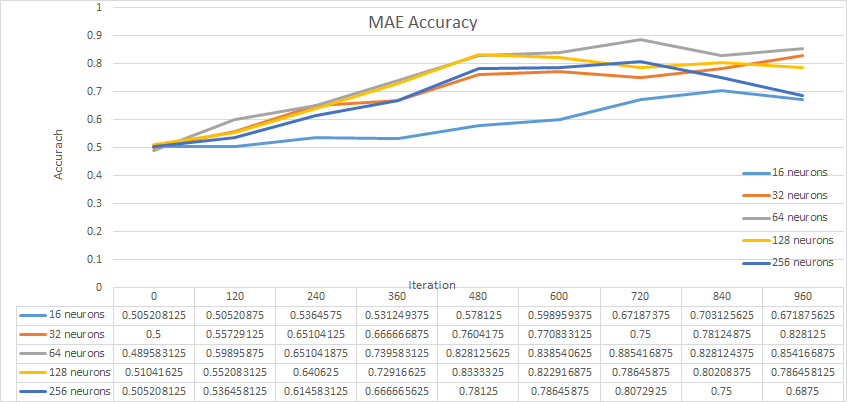
\includegraphics[width=\textwidth]{pictures/result_pictures/MAE_Accuracy.png}
    \caption{MAE Training Accuracy}
    \label{fig:mae_accuracy}
\end{figure}

\begin{figure}[t!]
    \centering
    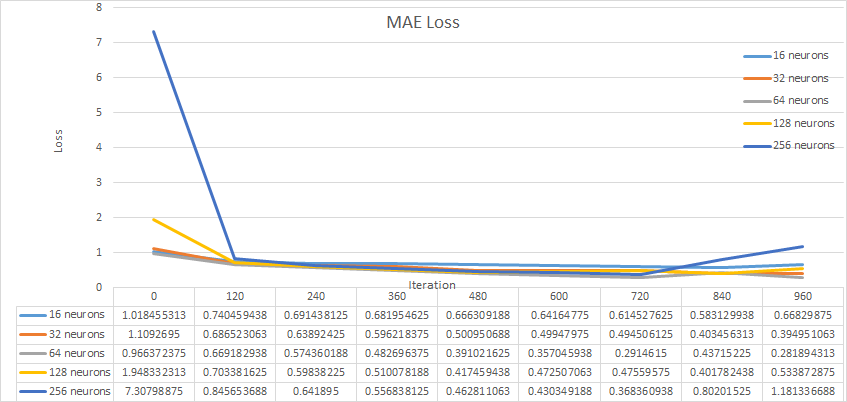
\includegraphics[width=\textwidth]{pictures/result_pictures/MAE_Loss.png}
    \caption{MAE Training Loss}
    \label{fig:mae_loss}
\end{figure}

\begin{table}[!t]
\centering
\caption{MAE, 16 Neuron Training Accuracy}
\label{tbl:mae_16_accuracy}
\resizebox{\textwidth}{!}{\begin{tabular}{|c|c|c|c|c|c|c|c|c|c|c|}
\hline
\multirow{2}{*}{Test} & \multirow{2}{*}{CV} & \multicolumn{9}{c|}{Iterations}                                                                                                         \\ \cline{3-11} 
                      &                     & 0           & 120           & 240           & 360           & 480           & 600          & 720          & 840          & 960          \\ \hline
\multirow{4}{*}{1}    & 1                   & 0.5         & 0.5           & 0.5           & 0.58333       & 0.58333       & 0.66667      & 0.58333      & 0.75         & 0.83333      \\ \cline{2-11} 
                      & 2                   & 0.5         & 0.5           & 0.66667       & 0.75          & 0.75          & 0.75         & 0.83333      & 0.91667      & 0.66667      \\ \cline{2-11} 
                      & 3                   & 0.5         & 0.5           & 0.5           & 0.5           & 0.5           & 0.5          & 0.66667      & 0.66667      & 0.66667      \\ \cline{2-11} 
                      & 4                   & 0.5         & 0.5           & 0.5           & 0.5           & 0.5           & 0.5          & 0.58333      & 0.58333      & 0.58333      \\ \hline
\multirow{4}{*}{2}    & 1                   & 0.5         & 0.5           & 0.5           & 0.41667       & 0.5           & 0.41667      & 0.58333      & 0.58333      & 0.58333      \\ \cline{2-11} 
                      & 2                   & 0.5         & 0.5           & 0.5           & 0.5           & 0.5           & 0.66667      & 0.58333      & 0.66667      & 0.66667      \\ \cline{2-11} 
                      & 3                   & 0.5         & 0.5           & 0.5           & 0.5           & 0.41667       & 0.5          & 0.5          & 0.41667      & 0.41667      \\ \cline{2-11} 
                      & 4                   & 0.58333     & 0.66667       & 0.58333       & 0.58333       & 0.66667       & 0.66667      & 0.83333      & 0.83333      & 0.75         \\ \hline
\multirow{4}{*}{3}    & 1                   & 0.5         & 0.5           & 0.5           & 0.5           & 0.66667       & 0.5          & 0.58333      & 0.58333      & 0.66667      \\ \cline{2-11} 
                      & 2                   & 0.5         & 0.5           & 0.58333       & 0.5           & 0.5           & 0.58333      & 0.75         & 0.66667      & 0.66667      \\ \cline{2-11} 
                      & 3                   & 0.5         & 0.5           & 0.5           & 0.5           & 0.58333       & 0.66667      & 0.75         & 0.83333      & 0.83333      \\ \cline{2-11} 
                      & 4                   & 0.5         & 0.5           & 0.33333       & 0.5           & 0.58333       & 0.41667      & 0.66667      & 0.66667      & 0.66667      \\ \hline
\multirow{4}{*}{4}    & 1                   & 0.5         & 0.5           & 0.58333       & 0.5           & 0.66667       & 0.66667      & 0.75         & 0.75         & 0.58333      \\ \cline{2-11} 
                      & 2                   & 0.5         & 0.5           & 0.58333       & 0.58333       & 0.58333       & 0.58333      & 0.66667      & 0.75         & 0.75         \\ \cline{2-11} 
                      & 3                   & 0.5         & 0.41667       & 0.66667       & 0.5           & 0.66667       & 0.66667      & 0.58333      & 0.66667      & 0.75         \\ \cline{2-11} 
                      & 4                   & 0.5         & 0.5           & 0.58333       & 0.58333       & 0.58333       & 0.83333      & 0.83333      & 0.91667      & 0.66667      \\ \hline
\multicolumn{2}{|c|}{Mean}                  & 0.505208125 & 0.50520875    & 0.5364575     & 0.531249375   & 0.578125      & 0.598959375  & 0.67187375   & 0.703125625  & 0.671875625  \\ \hline
\multicolumn{2}{|c|}{Std}                   & 0.0208325   & 0.04781121248 & 0.08032837701 & 0.07375412734 & 0.08855229679 & 0.1187070488 & 0.1074483726 & 0.1325280456 & 0.1030488131 \\ \hline
\end{tabular}}
\end{table}

\begin{table}[!t]
\centering
\caption{MAE, 32 Neuron Training Accuracy}
\label{tbl:mae_32_accuracy}
\resizebox{\textwidth}{!}{\begin{tabular}{|c|c|c|c|c|c|c|c|c|c|c|}
\hline
\multirow{2}{*}{Test} & \multirow{2}{*}{CV} & \multicolumn{9}{c|}{Iterations}                                                                                                     \\ \cline{3-11} 
                      &                     & 0             & 120        & 240          & 360          & 480          & 600          & 720          & 840          & 960          \\ \hline
\multirow{4}{*}{1}    & 1                   & 0.5           & 0.5        & 0.75         & 0.66667      & 0.75         & 0.83333      & 0.58333      & 0.58333      & 0.75         \\ \cline{2-11} 
                      & 2                   & 0.5           & 0.5        & 0.5          & 0.5          & 0.66667      & 0.75         & 0.75         & 0.83333      & 0.91667      \\ \cline{2-11} 
                      & 3                   & 0.41667       & 0.5        & 0.66667      & 0.66667      & 0.75         & 0.83333      & 0.83333      & 0.83333      & 0.83333      \\ \cline{2-11} 
                      & 4                   & 0.5           & 0.58333    & 0.75         & 0.58333      & 0.66667      & 0.75         & 0.75         & 0.83333      & 0.83333      \\ \hline
\multirow{4}{*}{2}    & 1                   & 0.5           & 0.5        & 0.5          & 0.5          & 0.75         & 0.5          & 0.66667      & 0.58333      & 0.66667      \\ \cline{2-11} 
                      & 2                   & 0.5           & 0.5        & 0.58333      & 0.66667      & 0.66667      & 0.75         & 0.75         & 0.75         & 0.83333      \\ \cline{2-11} 
                      & 3                   & 0.5           & 0.58333    & 0.75         & 0.75         & 1            & 1            & 0.91667      & 1            & 1            \\ \cline{2-11} 
                      & 4                   & 0.5           & 0.66667    & 0.75         & 0.83333      & 0.91667      & 0.5          & 0.5          & 0.75         & 0.75         \\ \hline
\multirow{4}{*}{3}    & 1                   & 0.58333       & 0.75       & 0.83333      & 0.66667      & 0.83333      & 0.75         & 0.5          & 0.5          & 0.66667      \\ \cline{2-11} 
                      & 2                   & 0.5           & 0.5        & 0.5          & 0.58333      & 0.75         & 0.75         & 0.75         & 0.91667      & 0.91667      \\ \cline{2-11} 
                      & 3                   & 0.5           & 0.5        & 0.5          & 0.5          & 0.5          & 0.66667      & 0.66667      & 0.58333      & 0.91667      \\ \cline{2-11} 
                      & 4                   & 0.5           & 0.5        & 0.66667      & 0.75         & 0.75         & 0.75         & 0.75         & 0.75         & 0.75         \\ \hline
\multirow{4}{*}{4}    & 1                   & 0.5           & 0.5        & 0.58333      & 0.66667      & 0.66667      & 0.83333      & 0.83333      & 0.83333      & 0.83333      \\ \cline{2-11} 
                      & 2                   & 0.5           & 0.5        & 0.58333      & 0.75         & 0.75         & 0.75         & 0.75         & 0.75         & 0.75         \\ \cline{2-11} 
                      & 3                   & 0.5           & 0.5        & 0.66667      & 0.75         & 0.83333      & 0.91667      & 1            & 1            & 1            \\ \cline{2-11} 
                      & 4                   & 0.5           & 0.83333    & 0.83333      & 0.83333      & 0.91667      & 1            & 1            & 1            & 0.83333      \\ \hline
\multicolumn{2}{|c|}{Mean}                  & 0.5           & 0.55729125 & 0.65104125   & 0.666666875  & 0.7604175    & 0.770833125  & 0.75         & 0.78124875   & 0.828125     \\ \hline
\multicolumn{2}{|c|}{Std}                   & 0.03042781381 & 0.1041662  & 0.1187071365 & 0.1097130939 & 0.1212393562 & 0.1410933825 & 0.1490711985 & 0.1577481878 & 0.1030493859 \\ \hline
\end{tabular}}
\end{table}

\begin{table}[!t]
\centering
\caption{MAE, 64 Neuron Training Accuracy}
\label{tbl:mae_64_accuracy}
\resizebox{\textwidth}{!}{\begin{tabular}{|c|c|c|c|c|c|c|c|c|c|c|}
\hline
\multirow{2}{*}{Test} & \multirow{2}{*}{CV} & \multicolumn{9}{c|}{Iterations}                                                                                                      \\ \cline{3-11} 
                      &                     & 0           & 120          & 240          & 360          & 480          & 600          & 720           & 840          & 960          \\ \hline
\multirow{4}{*}{1}    & 1                   & 0.5         & 0.66667      & 0.66667      & 0.75         & 0.91667      & 0.83333      & 0.91667       & 1            & 1            \\ \cline{2-11} 
                      & 2                   & 0.5         & 0.58333      & 0.66667      & 0.83333      & 0.91667      & 0.83333      & 0.91667       & 0.5          & 0.5          \\ \cline{2-11} 
                      & 3                   & 0.5         & 0.5          & 0.5          & 0.58333      & 0.66667      & 0.75         & 0.75          & 0.58333      & 0.66667      \\ \cline{2-11} 
                      & 4                   & 0.5         & 0.5          & 0.5          & 0.66667      & 0.75         & 0.75         & 0.83333       & 0.75         & 0.83333      \\ \hline
\multirow{4}{*}{2}    & 1                   & 0.5         & 0.66667      & 0.75         & 0.83333      & 1            & 1            & 1             & 1            & 1            \\ \cline{2-11} 
                      & 2                   & 0.5         & 0.5          & 0.5          & 0.75         & 0.83333      & 0.75         & 0.75          & 0.83333      & 0.83333      \\ \cline{2-11} 
                      & 3                   & 0.5         & 0.5          & 0.5          & 0.5          & 0.75         & 0.75         & 0.83333       & 0.75         & 0.75         \\ \cline{2-11} 
                      & 4                   & 0.5         & 0.83333      & 0.75         & 0.66667      & 0.91667      & 0.75         & 0.91667       & 0.91667      & 1            \\ \hline
\multirow{4}{*}{3}    & 1                   & 0.5         & 0.5          & 0.5          & 0.75         & 0.75         & 0.75         & 0.83333       & 1            & 0.83333      \\ \cline{2-11} 
                      & 2                   & 0.5         & 0.5          & 0.5          & 0.5          & 0.66667      & 0.75         & 0.75          & 0.75         & 0.75         \\ \cline{2-11} 
                      & 3                   & 0.5         & 0.5          & 0.5          & 0.75         & 0.58333      & 0.83333      & 0.83333       & 0.58333      & 0.66667      \\ \cline{2-11} 
                      & 4                   & 0.5         & 0.58333      & 0.66667      & 0.58333      & 0.83333      & 0.83333      & 0.91667       & 0.83333      & 1            \\ \hline
\multirow{4}{*}{4}    & 1                   & 0.5         & 0.66667      & 0.75         & 0.83333      & 0.83333      & 0.83333      & 0.91667       & 0.91667      & 0.91667      \\ \cline{2-11} 
                      & 2                   & 0.5         & 0.75         & 0.83333      & 0.91667      & 0.91667      & 1            & 1             & 1            & 1            \\ \cline{2-11} 
                      & 3                   & 0.5         & 0.66667      & 1            & 1            & 1            & 1            & 1             & 1            & 1            \\ \cline{2-11} 
                      & 4                   & 0.33333     & 0.66667      & 0.83333      & 0.91667      & 0.91667      & 1            & 1             & 0.83333      & 0.91667      \\ \hline
\multicolumn{2}{|c|}{Mean}                  & 0.489583125 & 0.59895875   & 0.651041875  & 0.739583125  & 0.828125625  & 0.838540625  & 0.885416875   & 0.828124375  & 0.854166875  \\ \hline
\multicolumn{2}{|c|}{Std}                   & 0.0416675   & 0.1063659607 & 0.1587526538 & 0.1486828436 & 0.1234868321 & 0.1030496217 & 0.09065183195 & 0.1651852566 & 0.1536588031 \\ \hline
\end{tabular}}
\end{table}

\begin{table}[!t]
\centering
\caption{MAE, 128 Neuron Training Accuracy}
\label{tbl:mae_128_accuracy}
\resizebox{\textwidth}{!}{\begin{tabular}{|c|c|c|c|c|c|c|c|c|c|c|}
\hline
\multirow{2}{*}{Test} & \multirow{2}{*}{CV} & \multicolumn{9}{c|}{Iterations}                                                                                                       \\ \cline{3-11} 
                      &                     & 0             & 120           & 240         & 360          & 480          & 600          & 720          & 840          & 960          \\ \hline
\multirow{4}{*}{1}    & 1                   & 0.5           & 0.66667       & 0.91667     & 0.75         & 0.75         & 0.75         & 0.91667      & 0.75         & 0.91667      \\ \cline{2-11} 
                      & 2                   & 0.5           & 0.5           & 0.66667     & 0.66667      & 0.83333      & 0.83333      & 0.91667      & 0.91667      & 0.91667      \\ \cline{2-11} 
                      & 3                   & 0.5           & 0.5           & 0.5         & 0.5          & 0.66667      & 0.66667      & 0.58333      & 0.75         & 0.75         \\ \cline{2-11} 
                      & 4                   & 0.5           & 0.58333       & 0.58333     & 0.91667      & 1            & 0.58333      & 0.5          & 0.5          & 0.5          \\ \hline
\multirow{4}{*}{2}    & 1                   & 0.5           & 0.5           & 0.5         & 0.5          & 0.75         & 0.75         & 0.5          & 0.75         & 0.83333      \\ \cline{2-11} 
                      & 2                   & 0.58333       & 0.5           & 0.5         & 0.58333      & 0.58333      & 0.83333      & 0.91667      & 1            & 0.75         \\ \cline{2-11} 
                      & 3                   & 0.5           & 0.5           & 0.5         & 0.5          & 0.75         & 0.91667      & 0.66667      & 0.75         & 0.83333      \\ \cline{2-11} 
                      & 4                   & 0.5           & 0.5           & 0.58333     & 0.83333      & 0.75         & 0.91667      & 0.58333      & 0.5          & 0.75         \\ \hline
\multirow{4}{*}{3}    & 1                   & 0.5           & 0.5           & 0.5         & 0.58333      & 0.83333      & 0.83333      & 0.75         & 0.75         & 0.75         \\ \cline{2-11} 
                      & 2                   & 0.5           & 0.5           & 0.5         & 0.75         & 0.75         & 0.75         & 0.83333      & 0.75         & 0.66667      \\ \cline{2-11} 
                      & 3                   & 0.5           & 0.58333       & 0.66667     & 0.75         & 1            & 0.66667      & 0.91667      & 0.91667      & 0.83333      \\ \cline{2-11} 
                      & 4                   & 0.5           & 0.5           & 0.58333     & 0.75         & 0.83333      & 0.91667      & 0.83333      & 0.58333      & 0.75         \\ \hline
\multirow{4}{*}{4}    & 1                   & 0.5           & 0.5           & 0.66667     & 0.83333      & 0.83333      & 0.83333      & 0.91667      & 1            & 0.5          \\ \cline{2-11} 
                      & 2                   & 0.58333       & 0.75          & 1           & 1            & 1            & 1            & 1            & 1            & 1            \\ \cline{2-11} 
                      & 3                   & 0.5           & 0.75          & 0.83333     & 0.91667      & 1            & 1            & 1            & 1            & 1            \\ \cline{2-11} 
                      & 4                   & 0.5           & 0.5           & 0.75        & 0.83333      & 1            & 0.91667      & 0.75         & 0.91667      & 0.83333      \\ \hline
\multicolumn{2}{|c|}{Mean}                  & 0.51041625    & 0.552083125   & 0.640625    & 0.72916625   & 0.8333325    & 0.822916875  & 0.78645875   & 0.80208375   & 0.786458125  \\ \hline
\multicolumn{2}{|c|}{Std}                   & 0.02846261358 & 0.09065106587 & 0.160205048 & 0.1595715908 & 0.1326372106 & 0.1212402154 & 0.1720496133 & 0.1717967953 & 0.1458332619 \\ \hline
\end{tabular}}
\end{table}

\begin{table}[!t]
\centering
\caption{MAE, 256 Neuron Training Accuracy}
\label{tbl:mae_256_accuracy}
\resizebox{\textwidth}{!}{\begin{tabular}{|c|c|c|c|c|c|c|c|c|c|c|}
\hline
\multirow{2}{*}{Test} & \multirow{2}{*}{CV} & \multicolumn{9}{c|}{Iterations}                                                                                                     \\ \cline{3-11} 
                      &                     & 0           & 120           & 240         & 360          & 480          & 600          & 720          & 840          & 960          \\ \hline
\multirow{4}{*}{1}    & 1                   & 0.5         & 0.5           & 0.66667     & 0.66667      & 0.75         & 0.66667      & 0.83333      & 0.83333      & 0.5          \\ \cline{2-11} 
                      & 2                   & 0.5         & 0.5           & 0.5         & 0.5          & 0.58333      & 0.5          & 0.5          & 0.75         & 0.75         \\ \cline{2-11} 
                      & 3                   & 0.5         & 0.5           & 0.5         & 0.58333      & 0.66667      & 0.66667      & 0.91667      & 0.91667      & 0.91667      \\ \cline{2-11} 
                      & 4                   & 0.5         & 0.5           & 0.75        & 0.58333      & 0.75         & 0.83333      & 0.58333      & 0.91667      & 0.5          \\ \hline
\multirow{4}{*}{2}    & 1                   & 0.5         & 0.5           & 0.5         & 0.5          & 0.75         & 0.75         & 0.75         & 0.5          & 0.5          \\ \cline{2-11} 
                      & 2                   & 0.5         & 0.5           & 0.5         & 0.5          & 0.5          & 0.66667      & 0.91667      & 0.83333      & 0.66667      \\ \cline{2-11} 
                      & 3                   & 0.5         & 0.5           & 0.5         & 0.75         & 0.75         & 0.83333      & 0.58333      & 0.66667      & 0.5          \\ \cline{2-11} 
                      & 4                   & 0.5         & 0.5           & 0.5         & 0.58333      & 0.83333      & 0.75         & 0.75         & 0.75         & 0.5          \\ \hline
\multirow{4}{*}{3}    & 1                   & 0.5         & 0.5           & 0.5         & 0.5          & 0.75         & 0.75         & 0.75         & 0.66667      & 0.83333      \\ \cline{2-11} 
                      & 2                   & 0.5         & 0.58333       & 0.91667     & 0.83333      & 0.91667      & 1            & 0.91667      & 0.58333      & 0.83333      \\ \cline{2-11} 
                      & 3                   & 0.5         & 0.5           & 0.58333     & 0.75         & 0.75         & 0.75         & 0.91667      & 0.91667      & 0.66667      \\ \cline{2-11} 
                      & 4                   & 0.5         & 0.5           & 0.58333     & 0.58333      & 0.75         & 0.75         & 0.75         & 0.5          & 0.58333      \\ \hline
\multirow{4}{*}{4}    & 1                   & 0.5         & 0.5           & 0.83333     & 0.83333      & 0.83333      & 0.91667      & 0.91667      & 0.83333      & 0.83333      \\ \cline{2-11} 
                      & 2                   & 0.5         & 0.83333       & 0.58333     & 0.75         & 0.91667      & 0.91667      & 0.91667      & 0.83333      & 0.91667      \\ \cline{2-11} 
                      & 3                   & 0.5         & 0.66667       & 0.66667     & 0.83333      & 1            & 1            & 1            & 0.5          & 0.5          \\ \cline{2-11} 
                      & 4                   & 0.58333     & 0.5           & 0.75        & 0.91667      & 1            & 0.83333      & 0.91667      & 1            & 1            \\ \hline
\multicolumn{2}{|c|}{Mean}                  & 0.505208125 & 0.536458125   & 0.614583125 & 0.666665625  & 0.78125      & 0.78645875   & 0.8072925    & 0.75         & 0.6875       \\ \hline
\multicolumn{2}{|c|}{Std}                   & 0.0208325   & 0.09112794984 & 0.135657299 & 0.1427249362 & 0.1356572478 & 0.1325275478 & 0.1481969411 & 0.1638655728 & 0.1813019785 \\ \hline
\end{tabular}}
\end{table}

%%%%%

\begin{table}[!t]
\centering
\caption{MAE, 16 Neuron Training Loss}
\label{tbl:mae_16_loss}
\resizebox{\textwidth}{!}{\begin{tabular}{|c|c|c|c|c|c|c|c|c|c|c|}
\hline
\multirow{2}{*}{Test} & \multirow{2}{*}{CV} & \multicolumn{9}{c|}{Iterations}                                                                                                           \\ \cline{3-11} 
                      &                     & 0            & 120           & 240           & 360           & 480           & 600           & 720          & 840          & 960          \\ \hline
\multirow{4}{*}{1}    & 1                   & 1.248406     & 0.700557      & 0.721534      & 0.683791      & 0.679869      & 0.671358      & 0.661637     & 0.64981      & 0.630611     \\ \cline{2-11} 
                      & 2                   & 0.81383      & 0.708748      & 0.668419      & 0.644472      & 0.608274      & 0.525449      & 0.432446     & 0.355196     & 0.660301     \\ \cline{2-11} 
                      & 3                   & 1.413861     & 0.86633       & 0.702162      & 0.717123      & 0.69526       & 0.695249      & 0.688936     & 0.683427     & 0.673695     \\ \cline{2-11} 
                      & 4                   & 1.187325     & 0.71034       & 0.718644      & 0.689946      & 0.691204      & 0.686907      & 0.685992     & 0.684144     & 0.682656     \\ \hline
\multirow{4}{*}{2}    & 1                   & 1.201566     & 0.727548      & 0.73316       & 0.701808      & 0.701004      & 0.696571      & 0.694853     & 0.692441     & 0.690223     \\ \cline{2-11} 
                      & 2                   & 0.815701     & 0.708713      & 0.695081      & 0.694276      & 0.689442      & 0.687621      & 0.685339     & 0.68283      & 0.680064     \\ \cline{2-11} 
                      & 3                   & 1.58734      & 0.892913      & 0.703405      & 0.718206      & 0.697049      & 0.698393      & 0.6957       & 0.694801     & 0.69378      \\ \cline{2-11} 
                      & 4                   & 0.683238     & 0.671772      & 0.649063      & 0.607525      & 0.548937      & 0.442233      & 0.391705     & 0.329769     & 0.441211     \\ \hline
\multirow{4}{*}{3}    & 1                   & 1.424314     & 0.916131      & 0.690333      & 0.711129      & 0.687896      & 0.689899      & 0.686423     & 0.685823     & 0.684495     \\ \cline{2-11} 
                      & 2                   & 0.820019     & 0.714047      & 0.690112      & 0.690204      & 0.685001      & 0.679225      & 0.670814     & 0.647553     & 0.616652     \\ \cline{2-11} 
                      & 3                   & 1.196719     & 0.726962      & 0.685195      & 0.685987      & 0.671463      & 0.668461      & 0.663434     & 0.657872     & 0.651768     \\ \cline{2-11} 
                      & 4                   & 0.816128     & 0.719749      & 0.692529      & 0.689858      & 0.687053      & 0.683292      & 0.680012     & 0.676621     & 0.672756     \\ \hline
\multirow{4}{*}{4}    & 1                   & 0.702769     & 0.697457      & 0.689328      & 0.681898      & 0.673521      & 0.6604        & 0.632447     & 0.540286     & 0.68499      \\ \cline{2-11} 
                      & 2                   & 0.956249     & 0.712512      & 0.670315      & 0.662117      & 0.654561      & 0.639672      & 0.610946     & 0.556251     & 0.496253     \\ \cline{2-11} 
                      & 3                   & 0.712369     & 0.687028      & 0.67461       & 0.664145      & 0.647231      & 0.609965      & 0.580946     & 0.581136     & 0.560655     \\ \cline{2-11} 
                      & 4                   & 0.715451     & 0.686544      & 0.67912       & 0.668789      & 0.643182      & 0.531669      & 0.370812     & 0.212119     & 1.17267      \\ \hline
\multicolumn{2}{|c|}{Mean}                  & 1.018455313  & 0.7404594375  & 0.691438125   & 0.681954625   & 0.6663091875  & 0.64164775    & 0.614527625  & 0.5831299375 & 0.66829875   \\ \hline
\multicolumn{2}{|c|}{Std}                   & 0.3006760362 & 0.07704728967 & 0.02146680104 & 0.02827351045 & 0.03985891142 & 0.07618871768 & 0.1124272118 & 0.1515363491 & 0.1535438104 \\ \hline
\end{tabular}}
\end{table}

\begin{table}[!t]
\centering
\caption{MAE, 32 Neuron Training Loss}
\label{tbl:mae_32_loss}
\resizebox{\textwidth}{!}{\begin{tabular}{|c|c|c|c|c|c|c|c|c|c|c|}
\hline
\multirow{2}{*}{Test} & \multirow{2}{*}{CV} & \multicolumn{9}{c|}{Iterations}                                                                                                         \\ \cline{3-11} 
                      &                     & 0            & 120           & 240           & 360           & 480          & 600          & 720          & 840          & 960          \\ \hline
\multirow{4}{*}{1}    & 1                   & 0.684434     & 0.654072      & 0.565662      & 0.65113       & 0.407152     & 0.498901     & 0.620457     & 0.623777     & 0.620168     \\ \cline{2-11} 
                      & 2                   & 0.772236     & 0.693365      & 0.685876      & 0.677614      & 0.665725     & 0.64133      & 0.556864     & 0.375201     & 0.158838     \\ \cline{2-11} 
                      & 3                   & 0.710254     & 0.663808      & 0.628011      & 0.575734      & 0.514098     & 0.473788     & 0.482586     & 0.389592     & 0.373604     \\ \cline{2-11} 
                      & 4                   & 0.807244     & 0.681819      & 0.66737       & 0.642006      & 0.584778     & 0.553336     & 0.514626     & 0.460837     & 0.394391     \\ \hline
\multirow{4}{*}{2}    & 1                   & 3.189419     & 0.694234      & 0.75583       & 0.715636      & 0.680119     & 0.682098     & 0.67483      & 0.670089     & 0.665802     \\ \cline{2-11} 
                      & 2                   & 0.710464     & 0.664054      & 0.628886      & 0.58269       & 0.522937     & 0.427006     & 0.581254     & 0.464811     & 0.422754     \\ \cline{2-11} 
                      & 3                   & 0.688761     & 0.669236      & 0.627207      & 0.506967      & 0.301451     & 0.136327     & 0.197662     & 0.088727     & 0.022258     \\ \cline{2-11} 
                      & 4                   & 0.696389     & 0.674154      & 0.638552      & 0.552976      & 0.231242     & 1.042702     & 0.682506     & 0.633012     & 0.627506     \\ \hline
\multirow{4}{*}{3}    & 1                   & 0.679018     & 0.6578        & 0.628541      & 0.566975      & 0.440659     & 0.420819     & 0.946089     & 0.643986     & 0.586387     \\ \cline{2-11} 
                      & 2                   & 0.770935     & 0.70297       & 0.692748      & 0.675768      & 0.627082     & 0.523196     & 0.445386     & 0.261977     & 0.298851     \\ \cline{2-11} 
                      & 3                   & 1.946271     & 0.787643      & 0.711192      & 0.718049      & 0.691005     & 0.684825     & 0.67681      & 0.663585     & 0.638306     \\ \cline{2-11} 
                      & 4                   & 0.72305      & 0.696589      & 0.682267      & 0.665598      & 0.645996     & 0.567738     & 0.525212     & 0.349333     & 0.517858     \\ \hline
\multirow{4}{*}{4}    & 1                   & 1.316252     & 0.797849      & 0.687329      & 0.614789      & 0.573686     & 0.516122     & 0.453537     & 0.393346     & 0.333136     \\ \cline{2-11} 
                      & 2                   & 2.309514     & 0.828695      & 0.645972      & 0.562575      & 0.491386     & 0.44171      & 0.406951     & 0.387647     & 0.369098     \\ \cline{2-11} 
                      & 3                   & 0.834531     & 0.640899      & 0.557031      & 0.489317      & 0.410021     & 0.291318     & 0.114176     & 0.032362     & 0.065739     \\ \cline{2-11} 
                      & 4                   & 0.90954      & 0.477182      & 0.420314      & 0.34167       & 0.227874     & 0.09046      & 0.033152     & 0.017019     & 0.224521     \\ \hline
\multicolumn{2}{|c|}{Mean}                  & 1.1092695    & 0.6865230625  & 0.63892425    & 0.596218375   & 0.5009506875 & 0.49947975   & 0.494506125  & 0.4034563125 & 0.3949510625 \\ \hline
\multicolumn{2}{|c|}{Std}                   & 0.7360253782 & 0.07856537831 & 0.07720142624 & 0.09694500948 & 0.1534492741 & 0.2234963677 & 0.2296608721 & 0.2183721905 & 0.2059401793 \\ \hline
\end{tabular}}
\end{table}

\begin{table}[!t]
\centering
\caption{MAE, 64 Neuron Training Loss}
\label{tbl:mae_64_loss}
\resizebox{\textwidth}{!}{\begin{tabular}{|c|c|c|c|c|c|c|c|c|c|c|}
\hline
\multirow{2}{*}{Test} & \multirow{2}{*}{CV} & \multicolumn{9}{c|}{Iterations}                                                                                                       \\ \cline{3-11} 
                      &                     & 0            & 120           & 240          & 360          & 480          & 600          & 720          & 840          & 960          \\ \hline
\multirow{4}{*}{1}    & 1                   & 0.708302     & 0.651603      & 0.613034     & 0.470021     & 0.339354     & 0.353478     & 0.230531     & 0.121292     & 0.095494     \\ \cline{2-11} 
                      & 2                   & 0.794855     & 0.670905      & 0.595705     & 0.318292     & 0.345416     & 0.252323     & 0.136917     & 1.786283     & 0.850147     \\ \cline{2-11} 
                      & 3                   & 1.237621     & 0.822646      & 0.677052     & 0.660906     & 0.634993     & 0.586031     & 0.463259     & 0.5823       & 0.412277     \\ \cline{2-11} 
                      & 4                   & 0.759072     & 0.733122      & 0.641733     & 0.613041     & 0.526007     & 0.404004     & 0.46646      & 0.470282     & 0.399456     \\ \hline
\multirow{4}{*}{2}    & 1                   & 0.826479     & 0.614915      & 0.445562     & 0.246747     & 0.149301     & 0.022201     & 0.010772     & 0.005466     & 0.00343      \\ \cline{2-11} 
                      & 2                   & 1.006263     & 0.700113      & 0.639816     & 0.564734     & 0.338585     & 0.564636     & 0.540944     & 0.446775     & 0.316585     \\ \cline{2-11} 
                      & 3                   & 0.679937     & 0.668232      & 0.659178     & 0.631523     & 0.571465     & 0.519896     & 0.394415     & 0.53157      & 0.625203     \\ \cline{2-11} 
                      & 4                   & 0.897283     & 0.642023      & 0.609337     & 0.54845      & 0.294037     & 0.454447     & 0.247062     & 0.128364     & 0.038323     \\ \hline
\multirow{4}{*}{3}    & 1                   & 0.86311      & 0.708145      & 0.686485     & 0.661283     & 0.616909     & 0.540987     & 0.396467     & 0.134488     & 0.228455     \\ \cline{2-11} 
                      & 2                   & 1.864664     & 0.759323      & 0.726964     & 0.679711     & 0.649054     & 0.633406     & 0.616398     & 0.59346      & 0.553221     \\ \cline{2-11} 
                      & 3                   & 0.836069     & 0.748321      & 0.675509     & 0.660153     & 0.64788      & 0.619508     & 0.54293      & 1.376405     & 0.539402     \\ \cline{2-11} 
                      & 4                   & 0.908264     & 0.672227      & 0.595384     & 0.56896      & 0.389971     & 0.392989     & 0.343517     & 0.258977     & 0.097075     \\ \hline
\multirow{4}{*}{4}    & 1                   & 1.411707     & 0.627432      & 0.44791      & 0.357645     & 0.314136     & 0.260436     & 0.217191     & 0.277396     & 0.164315     \\ \cline{2-11} 
                      & 2                   & 0.781084     & 0.63092       & 0.526501     & 0.42432      & 0.222934     & 0.009456     & 0.0044       & 0.000454     & 0.000245     \\ \cline{2-11} 
                      & 3                   & 1.006133     & 0.461931      & 0.186353     & 0.012467     & 0.001982     & 0.000847     & 0.000239     & 0.000196     & 0.000163     \\ \cline{2-11} 
                      & 4                   & 0.881115     & 0.595069      & 0.46324      & 0.304889     & 0.214322     & 0.09809      & 0.051882     & 0.280728     & 0.186518     \\ \hline
\multicolumn{2}{|c|}{Mean}                  & 0.966372375  & 0.6691829375  & 0.5743601875 & 0.482696375  & 0.391021625  & 0.3570459375 & 0.2914615    & 0.43715225   & 0.2818943125 \\ \hline
\multicolumn{2}{|c|}{Std}                   & 0.3055049074 & 0.08171502766 & 0.1351634195 & 0.1908280248 & 0.1976460417 & 0.2252874105 & 0.2088092583 & 0.4962797651 & 0.2585824134 \\ \hline
\end{tabular}}
\end{table}

\begin{table}[!t]
\centering
\caption{MAE, 128 Neuron Training Loss}
\label{tbl:mae_128_loss}
\resizebox{\textwidth}{!}{\begin{tabular}{|c|c|c|c|c|c|c|c|c|c|c|}
\hline
\multirow{2}{*}{Test} & \multirow{2}{*}{CV} & \multicolumn{9}{c|}{Iterations}                                                                                                     \\ \cline{3-11} 
                      &                     & 0           & 120          & 240          & 360          & 480          & 600          & 720          & 840          & 960          \\ \hline
\multirow{4}{*}{1}    & 1                   & 1.692298    & 0.641741     & 0.575657     & 0.485051     & 0.569813     & 0.463185     & 0.31271      & 0.41332      & 0.28579      \\ \cline{2-11} 
                      & 2                   & 2.012995    & 0.694935     & 0.649752     & 0.59163      & 0.509989     & 0.309364     & 0.256189     & 0.109023     & 0.493358     \\ \cline{2-11} 
                      & 3                   & 2.871913    & 0.795664     & 0.757398     & 0.689315     & 0.650009     & 0.616126     & 0.588173     & 0.474751     & 0.566887     \\ \cline{2-11} 
                      & 4                   & 0.757944    & 0.661073     & 0.590373     & 0.458398     & 0.124317     & 2.087584     & 1.603071     & 1.026679     & 0.775076     \\ \hline
\multirow{4}{*}{2}    & 1                   & 3.21693     & 0.716076     & 0.676173     & 0.662825     & 0.618064     & 0.569538     & 0.714131     & 0.611633     & 0.59248      \\ \cline{2-11} 
                      & 2                   & 0.709603    & 0.993861     & 0.648975     & 0.643298     & 0.617872     & 0.571356     & 0.484084     & 0.228748     & 0.611875     \\ \cline{2-11} 
                      & 3                   & 2.809269    & 0.718292     & 0.694279     & 0.665935     & 0.552694     & 0.323636     & 0.845132     & 0.519927     & 0.50351      \\ \cline{2-11} 
                      & 4                   & 1.482311    & 0.67491      & 0.64114      & 0.571785     & 0.498705     & 0.360266     & 0.783829     & 0.688235     & 0.54227      \\ \hline
\multirow{4}{*}{3}    & 1                   & 2.870377    & 0.783667     & 0.679531     & 0.623828     & 0.56877      & 0.465831     & 0.37696      & 0.46498      & 0.344629     \\ \cline{2-11} 
                      & 2                   & 1.404267    & 0.724492     & 0.652284     & 0.607433     & 0.575694     & 0.520558     & 0.451256     & 0.554169     & 0.56575      \\ \cline{2-11} 
                      & 3                   & 1.682552    & 0.673451     & 0.622202     & 0.562546     & 0.390985     & 0.459346     & 0.355144     & 0.17031      & 0.326592     \\ \cline{2-11} 
                      & 4                   & 0.705847    & 0.660663     & 0.606164     & 0.474036     & 0.286985     & 0.39726      & 0.221082     & 0.763939     & 0.618836     \\ \hline
\multirow{4}{*}{4}    & 1                   & 3.160802    & 0.898689     & 0.621886     & 0.510919     & 0.413852     & 0.262714     & 0.13664      & 0.04656      & 2.064901     \\ \cline{2-11} 
                      & 2                   & 2.066669    & 0.424045     & 0.218979     & 0.053586     & 0.00412      & 0.00091      & 0.000358     & 0.000232     & 0.00017      \\ \cline{2-11} 
                      & 3                   & 2.19558     & 0.513729     & 0.379848     & 0.184442     & 0.007359     & 0.000854     & 0.000119     & 0.000069     & 0.000058     \\ \cline{2-11} 
                      & 4                   & 1.53396     & 0.678818     & 0.559475     & 0.376224     & 0.290123     & 0.151585     & 0.480654     & 0.355944     & 0.249784     \\ \hline
\multicolumn{2}{|c|}{Mean}                  & 1.948332313 & 0.703381625  & 0.59838225   & 0.5100781875 & 0.4174594375 & 0.4725070625 & 0.47559575   & 0.4017824375 & 0.533872875  \\ \hline
\multicolumn{2}{|c|}{Std}                   & 0.853207409 & 0.1321884662 & 0.1296224218 & 0.1770240103 & 0.215715663  & 0.4697376952 & 0.3918787237 & 0.2960299259 & 0.4629277242 \\ \hline
\end{tabular}}
\end{table}

\begin{table}[!t]
\centering
\caption{MAE, 256 Neuron Training Loss}
\label{tbl:mae_256_loss}
\resizebox{\textwidth}{!}{\begin{tabular}{|c|c|c|c|c|c|c|c|c|c|c|}
\hline
\multirow{2}{*}{Test} & \multirow{2}{*}{CV} & \multicolumn{9}{c|}{Iterations}                                                                                                  \\ \cline{3-11} 
                      &                     & 0           & 120          & 240          & 360          & 480          & 600          & 720          & 840        & 960         \\ \hline
\multirow{4}{*}{1}    & 1                   & 3.150867    & 0.735766     & 0.644316     & 0.620983     & 0.590476     & 0.522656     & 0.457039     & 0.407634   & 3.857999    \\ \cline{2-11} 
                      & 2                   & 5.721464    & 1.912743     & 0.995055     & 0.727561     & 0.678332     & 0.68497      & 0.668271     & 0.658809   & 0.648772    \\ \cline{2-11} 
                      & 3                   & 8.916656    & 0.862466     & 0.709399     & 0.638999     & 0.596239     & 0.553562     & 0.471526     & 0.385455   & 0.273993    \\ \cline{2-11} 
                      & 4                   & 9.137609    & 0.84617      & 0.610897     & 0.58117      & 0.515767     & 0.395379     & 0.508983     & 0.232883   & 5.799033    \\ \hline
\multirow{4}{*}{2}    & 1                   & 7.54897     & 0.714874     & 0.6908       & 0.665917     & 0.616479     & 0.565999     & 0.425728     & 1.153986   & 0.657882    \\ \cline{2-11} 
                      & 2                   & 9.482568    & 0.678529     & 0.809575     & 0.673676     & 0.614241     & 0.567809     & 0.508461     & 0.405226   & 0.662943    \\ \cline{2-11} 
                      & 3                   & 8.208381    & 0.699572     & 0.710194     & 0.606328     & 0.569183     & 0.499355     & 0.475914     & 0.585483   & 0.758418    \\ \cline{2-11} 
                      & 4                   & 9.232345    & 1.169096     & 0.69612      & 0.623307     & 0.5693       & 0.517541     & 0.447053     & 0.353785   & 2.103675    \\ \hline
\multirow{4}{*}{3}    & 1                   & 8.666858    & 0.993195     & 0.771614     & 0.706089     & 0.638598     & 0.612379     & 0.567323     & 0.510867   & 0.432677    \\ \cline{2-11} 
                      & 2                   & 6.069348    & 0.595496     & 0.367613     & 0.535616     & 0.22024      & 0.127649     & 0.19117      & 0.610151   & 0.463563    \\ \cline{2-11} 
                      & 3                   & 6.6591      & 0.773798     & 0.631237     & 0.489065     & 0.320229     & 0.361781     & 0.20733      & 0.13806    & 0.595329    \\ \cline{2-11} 
                      & 4                   & 7.98459     & 0.694867     & 0.655305     & 0.631581     & 0.564609     & 0.564327     & 0.478051     & 1.848759   & 0.620344    \\ \hline
\multirow{4}{*}{4}    & 1                   & 9.34032     & 0.672664     & 0.509447     & 0.373011     & 0.267692     & 0.198101     & 0.13534      & 0.644929   & 0.37846     \\ \cline{2-11} 
                      & 2                   & 8.789352    & 0.57045      & 0.553231     & 0.433809     & 0.355714     & 0.264717     & 0.143217     & 0.317178   & 0.205836    \\ \cline{2-11} 
                      & 3                   & 6.999865    & 0.691546     & 0.51303      & 0.379677     & 0.18769      & 0.04563      & 0.000372     & 4.484148   & 1.409804    \\ \cline{2-11} 
                      & 4                   & 1.019527    & 0.919227     & 0.402487     & 0.222621     & 0.100188     & 0.403732     & 0.207997     & 0.094891   & 0.032659    \\ \hline
\multicolumn{2}{|c|}{Mean}                  & 7.30798875  & 0.8456536875 & 0.641895     & 0.556838125  & 0.4628110625 & 0.4303491875 & 0.3683609375 & 0.80201525 & 1.181336688 \\ \hline
\multicolumn{2}{|c|}{Std}                   & 2.384098207 & 0.3234293831 & 0.1549271033 & 0.1409353488 & 0.1879214812 & 0.1856378876 & 0.190433357  & 1.07015756 & 1.546361786 \\ \hline
\end{tabular}}
\end{table}

\subsection{Error from AE in {\em second model} and {\em third model}}
Table \ref{tbl:sae_error} and Table \ref{tbl:mae_error} show error from AE. The error function $E()$ is defined as following:
$$E(\vec{x}, \vec{d})=\sum_k(x_i-d_i)^2$$
where $\vec{x}$ is input signal, $\vec{d}$ is output signal from last decoder. The total average error from AE in {\em second model} is 0.1587907 and the total average error from AE in {\em third model} is 0.1720756. Both error are big enough to affect performance because most range of standardized data for experiments is between 3 and -3. Figure \ref{fig:sae_error_c3}, Figure \ref{fig:sae_error_c17}, Figure \ref{fig:mae_error_c3}, and Figure \ref{fig:mae_error_c17} help visualize error.

Such big error between original input and output from decode layer implies that data from final encode layer also has big error. The error in encoded data can interrupt train followed neural networks. In this case, the error interrupts LSTM layer.


\begin{table}[!t]
\centering
\caption{Error from AE in {\em second model}}
\label{tbl:sae_error}
\begin{tabular}{|c|c|c|c|c|c|c|}
\hline
\multirow{2}{*}{Test} & \multirow{2}{*}{CV} & \multicolumn{5}{c|}{The number of neurans}                                   \\ \cline{3-7} 
                      &                     & 16            & 32            & 64            & 128           & 256          \\ \hline
\multirow{4}{*}{1}    & 1                   & 0.178460395   & 0.1239250116  & 0.1748844814  & 0.1502201539  & 0.1886790823 \\ \cline{2-7} 
                      & 2                   & 0.1658136155  & 0.1384476442  & 0.102677634   & 0.2454849277  & 0.1165074687 \\ \cline{2-7} 
                      & 3                   & 0.1409358419  & 0.1701477412  & 0.1447305065  & 0.1517742854  & 0.1233751141 \\ \cline{2-7} 
                      & 4                   & 0.13444083    & 0.1528848018  & 0.1856264398  & 0.1555761881  & 0.1862711851 \\ \hline
\multirow{4}{*}{2}    & 1                   & 0.1573844403  & 0.1424119417  & 0.1411998086  & 0.1525888257  & 0.1580447592 \\ \cline{2-7} 
                      & 2                   & 0.141391445   & 0.1517100111  & 0.1507830191  & 0.1466212031  & 0.1407112777 \\ \cline{2-7} 
                      & 3                   & 0.1822773032  & 0.1744369417  & 0.1704759225  & 0.2495105062  & 0.1746258009 \\ \cline{2-7} 
                      & 4                   & 0.1417274438  & 0.1453869026  & 0.1316085961  & 0.1373841651  & 0.1503036991 \\ \hline
\multirow{4}{*}{3}    & 1                   & 0.1496374961  & 0.1435624324  & 0.1280109156  & 0.1312412135  & 0.1869615819 \\ \cline{2-7} 
                      & 2                   & 0.1594685651  & 0.1389588062  & 0.1716334522  & 0.114069676   & 0.166966049  \\ \cline{2-7} 
                      & 3                   & 0.2582480293  & 0.158985598   & 0.1400841698  & 0.1527932584  & 0.1612278037 \\ \cline{2-7} 
                      & 4                   & 0.157985406   & 0.156085087   & 0.1775525697  & 0.2080688961  & 0.1272955388 \\ \hline
\multirow{4}{*}{4}    & 1                   & 0.1478289105  & 0.3086702116  & 0.1200938132  & 0.140119426   & 0.179127017  \\ \cline{2-7} 
                      & 2                   & 0.1227029786  & 0.1786029078  & 0.1612949632  & 0.1493861414  & 0.1175681986 \\ \cline{2-7} 
                      & 3                   & 0.2519034538  & 0.1407385003  & 0.2101189978  & 0.1865597609  & 0.1705561783 \\ \cline{2-7} 
                      & 4                   & 0.1378952377  & 0.1178480741  & 0.1207066998  & 0.1200009286  & 0.1612533517 \\ \hline
\multicolumn{2}{|c|}{Mean}                  & 0.164256337   & 0.1589251633  & 0.1519676243  & 0.1619624723  & 0.1568421316 \\ \hline
\multicolumn{2}{|c|}{Std}                   & 0.03874978321 & 0.04322578706 & 0.02855709465 & 0.04024832136 & 0.0250276511 \\ \hline
\end{tabular}
\end{table}

\begin{table}[!t]
\centering
\caption{Error from AE in {\em third model}}
\label{tbl:mae_error}
\begin{tabular}{|c|c|c|c|c|c|c|}
\hline
\multirow{2}{*}{Test} & \multirow{2}{*}{CV} & \multicolumn{5}{c|}{The number of neurans}                                   \\ \cline{3-7} 
                      &                     & 16           & 32            & 64            & 128           & 256           \\ \hline
\multirow{4}{*}{1}    & 1                   & 0.1731109992 & 0.1436949167  & 0.1456636973  & 0.187595576   & 0.151621541   \\ \cline{2-7} 
                      & 2                   & 0.2256366871 & 0.2343511172  & 0.225972496   & 0.1990794409  & 0.1417004224  \\ \cline{2-7} 
                      & 3                   & 0.1696365457 & 0.1366730388  & 0.1627431139  & 0.2070423551  & 0.1462982614  \\ \cline{2-7} 
                      & 4                   & 0.1305910405 & 0.1537955459  & 0.1439991277  & 0.1212673876  & 0.2361955196  \\ \hline
\multirow{4}{*}{2}    & 1                   & 0.1933368258 & 0.2014074977  & 0.1557413656  & 0.1772724874  & 0.1504026726  \\ \cline{2-7} 
                      & 2                   & 0.194492355  & 0.1620466933  & 0.186969487   & 0.1627819967  & 0.1599432845  \\ \cline{2-7} 
                      & 3                   & 0.1982949749 & 0.1404892672  & 0.1382220406  & 0.1454426982  & 0.2511638664  \\ \cline{2-7} 
                      & 4                   & 0.1465102062 & 0.161547171   & 0.2015030943  & 0.2068295442  & 0.1813242622  \\ \hline
\multirow{4}{*}{3}    & 1                   & 0.1649940163 & 0.1923567355  & 0.1391313598  & 0.1653740592  & 0.1548881214  \\ \cline{2-7} 
                      & 2                   & 0.181799693  & 0.1197193041  & 0.2793735377  & 0.2084757499  & 0.1446572952  \\ \cline{2-7} 
                      & 3                   & 0.1511649378 & 0.1994536668  & 0.1662912238  & 0.1363047659  & 0.2827695534  \\ \cline{2-7} 
                      & 4                   & 0.1715208553 & 0.1815536954  & 0.1574255787  & 0.1797324885  & 0.1525612958  \\ \hline
\multirow{4}{*}{4}    & 1                   & 0.139421409  & 0.179470161   & 0.1902030185  & 0.1344845295  & 0.154265251   \\ \cline{2-7} 
                      & 2                   & 0.157693075  & 0.1295783296  & 0.1185395364  & 0.1784827951  & 0.2548566163  \\ \cline{2-7} 
                      & 3                   & 0.2060995549 & 0.1818246227  & 0.1764678694  & 0.2163151987  & 0.1157963872  \\ \cline{2-7} 
                      & 4                   & 0.1625140198 & 0.1539499387  & 0.1419902053  & 0.1478702892  & 0.1442933325  \\ \hline
\multicolumn{2}{|c|}{Mean}                  & 0.1729260747 & 0.1669944813  & 0.170639797   & 0.1733969601  & 0.1764211052  \\ \hline
\multicolumn{2}{|c|}{Std}                   & 0.0258008777 & 0.03077204756 & 0.03992570438 & 0.02998005823 & 0.05004155784 \\ \hline
\end{tabular}
\end{table}

\begin{figure}[t!]
    \centering
    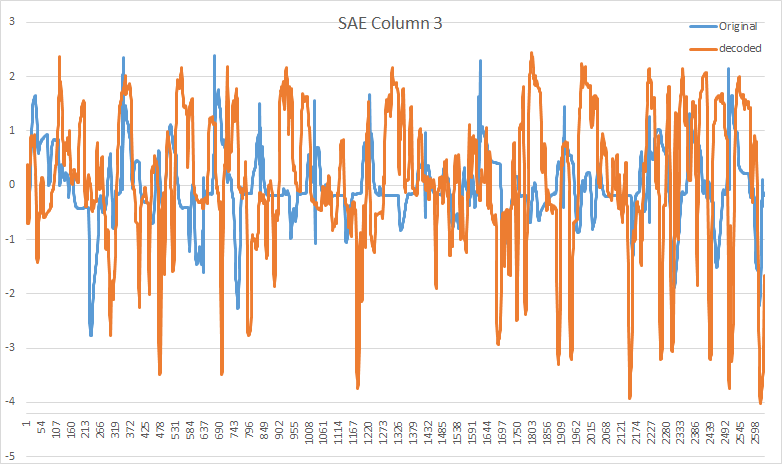
\includegraphics[width=\textwidth]{pictures/result_pictures/SAE_Column_3.png}
    \caption{SAE, AE Error for Column 3}
    \label{fig:sae_error_c3}
\end{figure}

\begin{figure}[t!]
    \centering
    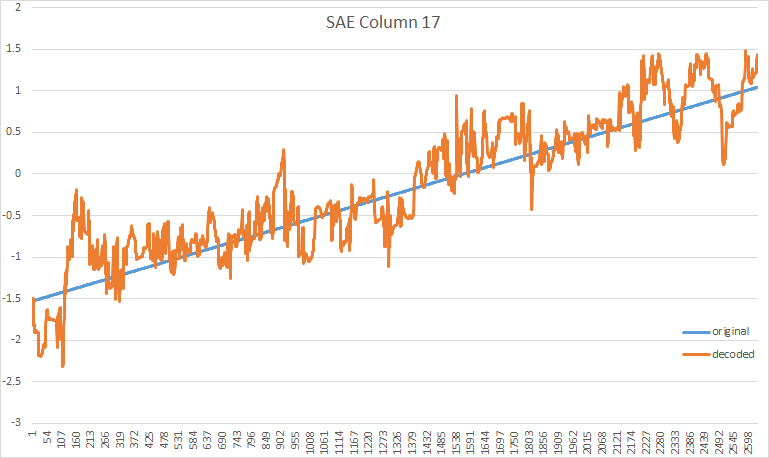
\includegraphics[width=\textwidth]{pictures/result_pictures/SAE_Column_17.png}
    \caption{SAE, AE Error for Column 17}
    \label{fig:sae_error_c17}
\end{figure}

\begin{figure}[t!]
    \centering
    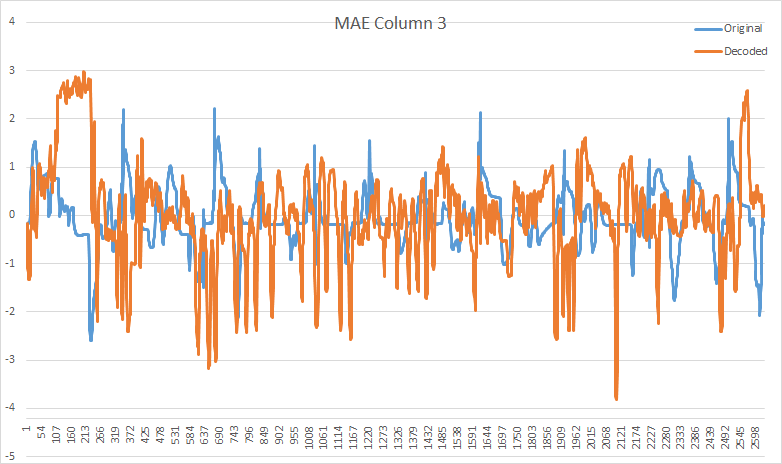
\includegraphics[width=\textwidth]{pictures/result_pictures/MAE_Column_3.png}
    \caption{MAE, AE Error for Column 3}
    \label{fig:mae_error_c3}
\end{figure}

\begin{figure}[t!]
    \centering
    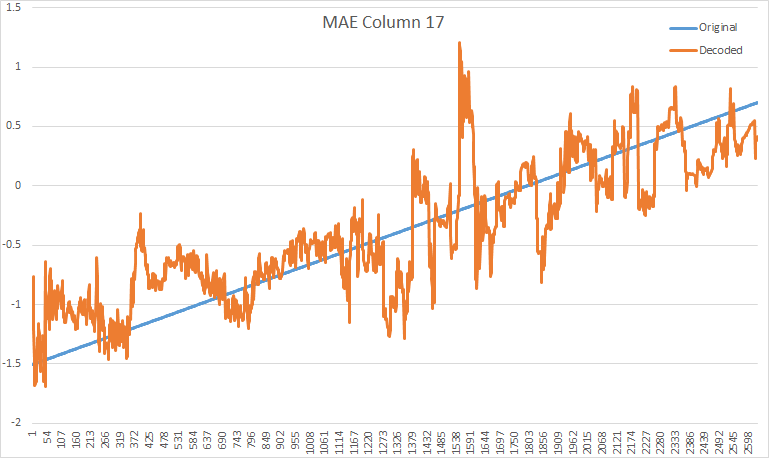
\includegraphics[width=\textwidth]{pictures/result_pictures/MAE_Column_17.png}
    \caption{MAE, AE Error for Column 17}
    \label{fig:mae_error_c17}
\end{figure}

% ####################################################################################################################################
\chapter{Conclusion and Future work}\label{chap:conclusion}
% ####################################################################################################################################
\section{Data Size}
Two different data sizes should be considered on this paper. First data size is number of samples in each traces. Data with more samples in each traces gave better performance from first part of experiments with {\em first model}. The average accuracy with 1 over 10 sampled data show higher accuracy than the average accuracy with 1 over 20 sampled data and 1 over 50 sampled data. From the fact, experiments with more sample, data without re-sampling or data from long driving time, are expected with better performance. 

Another data size is the number of traces. All experiments on the paper used 16 traces. The 12 traces were used for training and the 4 traces were used for testing. The 12 traces were not enough to train neural networks: {\em first model}, {\em second model}, and {\em third model}. Especially, {\em second model} and {\em third model} need more data than {\em first model} because two models are more complex than {\em first model}. To train complex neural network needs more data. Next experiments in the future should use data with enough sample in each traces and enough number of traces. 

\section{Limitation of Auto-encoder}
The result from experiments with with SAE in {\em second model} and MAE in {\em third model} show bad performance. The principle of AE is to find two matrices: first matrix is used for compression and second matrix is used for decompression. If two matrices are not exist, impossible to reduce original dimensions to target dimensions, either SAE or MAE do not work. For example, during training first layer of MAE in {\em third model} which reduced 98 features to 75 features, error from this was less than 0.009. This is much better performance than reducing 98 dimensions to 25 dimensions. Therefore, the bad performance of AE implies that it is not possible to reduce 98 features of original data to 25 features by AE.

The second limitation of AE is that auto-encoder always tries to keep all information on encoded data. It means that auto-encoder cannot remove unimportant features as principal components analysis (PCA) does. PCA is another popular method to reduce dimensions. It first takes a feature which has more information than other features. With the {\em raw dataset}, PCA is better method than AE because {\em raw dataset} has many unnecessary features.

For future work, it is necessary to research AE for reducing dimensions with ability to ignore unimportant features and keep information from important features.

\section{Training Multiple Layer Auto-encoder}
Chapter \ref{subsubsec:MAE} explains how to train MAE based on \cite{hinton2006reducing}. The paper introduces pretraining process, and it can help initialize good weights. However, processing of pretraining takes really long time. For example, average testing time for {\em third model} with 256 neurons took 10 hours and 27 minutes but testing time for {\em second model} with 256 neurons took 8 hours and 33 minutes. The process of pretraining took about 2 hours.

Unlikely train each layer separately in pretraining, add more AE untill it gives big error or it reaches goal dimensions. Figure \ref{fig:train_NMAE1}, Figure \ref{fig:train_NMAE2}, and Figure \ref{fig:train_NMAE3} show how to train MAE.

	Figure \ref{fig:train_NMAE1} shows SAE and its error function is
$$E(\vec{x}, \bold{g_1}(\bold{f_1}(\vec{X}\bold{E_1})\bold{D_1}))$$
Now if it gives small enough error, add one more layer as Figure \ref{fig:train_NMAE2}. In this case, the error function is
$$E(\vec{x}, \bold{g_1}(\bold{g_2}(\bold{f_2}(\bold{f_1}(\vec{X}\bold{E_1})\bold{E_2})\bold{D_2})\bold{D_1}))$$
If it also gives small enough error, add one more layer as Figure \ref{fig:train_NMAE3}. In this case, the error function is
$$E(\vec{x}, \bold{g_1}(\bold{g_2}(\bold{g_3}(\bold{f_3}(\bold{f_2}(\bold{f_1}(\vec{X}\bold{E_1})\bold{E_2})\bold{E_3})\bold{D_3})\bold{D_2})\bold{D_1}))$$
If it does not give small error, stop adding more layer.

This way can give two benefits. First benefit is to save train time. To compare with method on \cite{hinton2006reducing}, it does not train whole network because this way always train whole network. Another benefit is to find dimensions how much AE can reduce. For the future work, it is worth to compare two different train methods for MAE and find minimize dimensions reduced by AE.

\begin{figure}[t!]
    \centering
    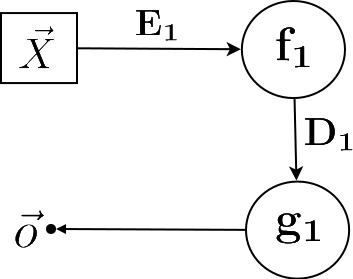
\includegraphics[width=0.3\textwidth]{pictures/figures/train_new_MAE1.png}
    \caption{First Step of New Way to train MAE}
    \label{fig:train_NMAE1}
\end{figure}

\begin{figure}[t!]
    \centering
    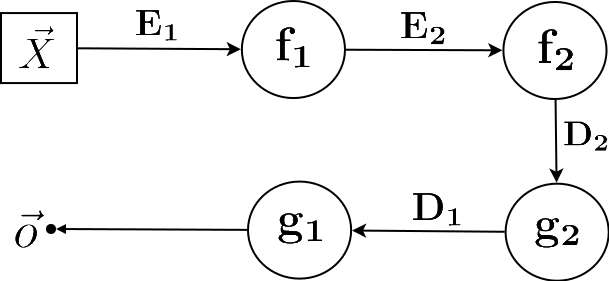
\includegraphics[width=0.5\textwidth]{pictures/figures/train_new_MAE2.png}
    \caption{Second Step of New Way to train MAE}
    \label{fig:train_NMAE2}
\end{figure}

\begin{figure}[t!]
    \centering
    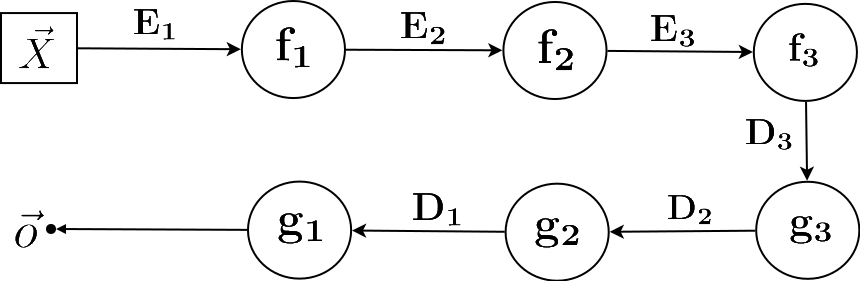
\includegraphics[width=0.75\textwidth]{pictures/figures/train_new_MAE3.png}
    \caption{Thrid Step of New Way to train MAE}
    \label{fig:train_NMAE3}
\end{figure}




\end{thesis}

\bibliography{references.bib}

\end{document}
\endinput
